\chapter{Memory Management and Protection}

\section{Context and Goals}

At the end of Week 3 the kernel was small but working: unprivileged code reached the hardware only through system calls (\texttt{svc}). \textbf{Memory}, however, was completely open. The kernel's variables, the application's variables and every stack lived side by side in the same RAM, and unprivileged mode, which blocks certain instructions and the system registers, does not check ordinary loads and stores. The question of this week is therefore: \textbf{who may touch which memory?} The answer comes in three steps:

\begin{enumerate}
    \item \textbf{Unit 1: Memory management -- the ideas.} Why an operating system manages memory, static versus dynamic allocation, and the spectrum from flat memory to paging and virtual memory (page tables, TLB, page faults, effective access time), ending with MMU versus MPU. No code: you observe the starting code and see what it fails to protect.
    \item \textbf{Unit 2: Task partitions.} Each task gets its own 4 KB slice of RAM, placed by the linker, with its stack at the bottom. The kernel starts a task on its own \textbf{Process Stack Pointer (PSP)} and ends it cleanly.
    \item \textbf{Unit 3: The MPU.} You program the Cortex-M3 \textbf{Memory Protection Unit}, so that the hardware stops any task that accesses memory outside its partition, and the kernel checks every pointer that a task passes to it.
\end{enumerate}

\section{Where You Start}

The code is in two sibling directories, \texttt{week-04/base/} and \texttt{week-04/solution/}, each with its own \texttt{Makefile}. You start in \texttt{base/} and turn it step by step into \texttt{solution/}. Unless otherwise specified, all paths in these notes are relative to \texttt{week-04/solution/}; QEMU runs with \texttt{-nographic} and is stopped with \texttt{Ctrl-C}.

Unlike Week 3, the base \textbf{builds and runs from the first minute}. It already runs two unprivileged tasks, Task A and then Task B, each with its own stack, but without any partitioning or protection. The long parts that are not the focus of this week are already prepared:
\begin{itemize}
    \item the task table and the code that starts and ends a task (\texttt{kernel/task.c});
    \item an \texttt{SVC\_Handler} that finds the system-call frame on either the MSP or the PSP, and the new system call \texttt{sys\_exit};
    \item the CMSIS definitions of the MPU registers and of \texttt{MMFAR} (\texttt{include/cmsdk.h});
    \item the two applications (\texttt{src/task\_a.c}, \texttt{src/task\_b.c}) and the \texttt{DEMO} switch of the \texttt{Makefile}.
\end{itemize}

What you write is about sixty lines: in \textbf{Unit 2} the partition block of the linker script (\texttt{scripts/mps2\_m3.ld}); in \textbf{Unit 3} the two MPU functions (\texttt{kernel/mpu.c}), the address report in \texttt{MemManage\_Handler} (\texttt{kernel/faults.c}) and the pointer check in \texttt{sys\_write\_impl} (\texttt{kernel/syscall.c}).

\subsection{The DEMO Switch}

\texttt{make run DEMO=}\textit{name} builds Task B with a block of deliberate misbehavior, included through a preprocessor test such as \texttt{\#if defined(DEMO\_ROGUE)} in \texttt{src/task\_b.c}. Each demo is built in its own directory (for example \texttt{build/demo-rogue/}), so switching between demos never needs a \texttt{make clean}; a plain \texttt{make run} builds the normal program in \texttt{build/}. The three demos are:

\begin{itemize}
    \item \texttt{rogue}: B writes directly into the kernel's uptime counter;
    \item \texttt{badptr}: B passes a kernel address to \texttt{sys\_write};
    \item \texttt{overflow}: B recurses until its stack grows out of its own memory.
\end{itemize}

Running them on the base, after the partitions and after the MPU shows what each layer of protection can and cannot prevent. Note that a \textbf{correct} program prints the same output at every stage: what changes is what a \textbf{wrong} or malicious program is allowed to do.

\section{Unit 1: Memory Management -- the Ideas}

\subsection{Why an Operating System Manages Memory}

Memory is one shared resource that several programs want at once: the kernel and every task. An operating system has four jobs with respect to memory:

\begin{itemize}
    \item \textbf{Placement.} Decide where each program's code, data and stack go, so that they do not overlap. Two programs that both think they own \texttt{0x20000004} would destroy each other's data.
    \item \textbf{Sharing.} Let programs use the same memory when they should: one copy of a library serves every program, a buffer can be handed to a device, two programs can exchange data through a common area.
    \item \textbf{Protection.} Stop a program from reading or writing memory that is not its own, by mistake (a bad pointer, a stack that grows too far) or on purpose.
    \item \textbf{More programs than memory.} When the programs together need more than the RAM available, keep in RAM only the parts in use and the rest somewhere else.
\end{itemize}

In this unit you write no code. You look at the starting code and see which jobs it does. The short answer: only the first, and only partly.

\subsection{What the Starting Code Does}

\textbf{Placement.} In \texttt{week-04/base/}, build the program and ask binutils where the linker put four variables: \texttt{uptime\_ms} and \texttt{tx\_buf} (kernel), \texttt{a\_lines} (Task A) and \texttt{b\_seconds} (Task B):

\begin{lstlisting}[language=bash]
make
arm-none-eabi-nm -n build/scratch-os.axf | grep -E ' (uptime_ms|tx_buf|a_lines|b_seconds)\$'
\end{lstlisting}

\begin{lstlisting}
20000004 B uptime_ms
20000008 b tx_buf
20000054 b a_lines
20000058 b b_seconds
\end{lstlisting}

The letter is the symbol type: \texttt{B}/\texttt{b} means \texttt{.bss} (upper case for global, lower case for \texttt{static}). The space before the names and the \texttt{\$} after them keep only whole names; otherwise \texttt{systick\_uptime\_ms} would match too. All four variables are packed together just above \texttt{0x20000000}, and there is \textbf{no border} between kernel and task data: the linker placed them file after file, with the generic \texttt{*(.bss*)} rule. If Task B computed \texttt{0x20000054} and wrote there, it would change A's variable and nobody would notice. The starting code does placement only, per variable and not per task.

\textbf{Behavior.} \texttt{make run} (watch about six seconds, then \texttt{Ctrl-C}) prints:

\begin{lstlisting}
scratch-os: kernel started
starting task A
A: hello from task A
A: uptime 0 ms (line 1)
A: uptime 1000 ms (line 2)
A: uptime 2000 ms (line 3)
task A exited
starting task B
B: hello from task B
B: uptime 4000 ms (second 1)
B: uptime 5000 ms (second 2)
B: uptime 6000 ms (second 3)
\end{lstlisting}

A runs to its end, then B starts: the two tasks \textbf{never run at the same time}. B's first line says \texttt{4000 ms} because the uptime is the kernel's clock since boot: B starts at about 3000 ms, after A's three waits, and prints one second later. The same output is printed by the finished program: a correct program does not change, only a wrong one does.

\textbf{The board's memory.} In QEMU's monitor, \texttt{info mtree -f} lists the memories. What the linker script calls FLASH is \texttt{mps.ssram1} at \texttt{0x00000000}, 4 MiB; what it calls RAM is \texttt{mps.ssram23} at \texttt{0x20000000}, 4 MiB; both also appear at \texttt{+0x400000} (an \textbf{alias}: the same bytes at a second address). The list says every memory is just \texttt{ram}: nothing says who may access it. The bus answers any load or store from any code, privileged or not, so protection must come from somewhere else.

\subsection{Static versus Dynamic Allocation}

The other half of placement is \textbf{when} addresses are decided.

\begin{itemize}
    \item \textbf{Static allocation} fixes every address and size at \textbf{link time}. The map file shows the whole layout before the program runs and no holes appear, because nothing is freed. The price is flexibility: sizes cannot change at run time.
    \item \textbf{Dynamic allocation} hands out memory at \textbf{run time} from a \textbf{heap} (\texttt{malloc}/\texttt{free}). It is flexible, but the layout depends on the order of the calls. After many allocations and frees, free memory is split into small \textbf{holes}: with 4 free blocks in total but no hole of 3, a request for 3 blocks \textbf{fails} although memory is free (\textbf{external fragmentation}).
\end{itemize}

\begin{figure}[h]
    \centering
    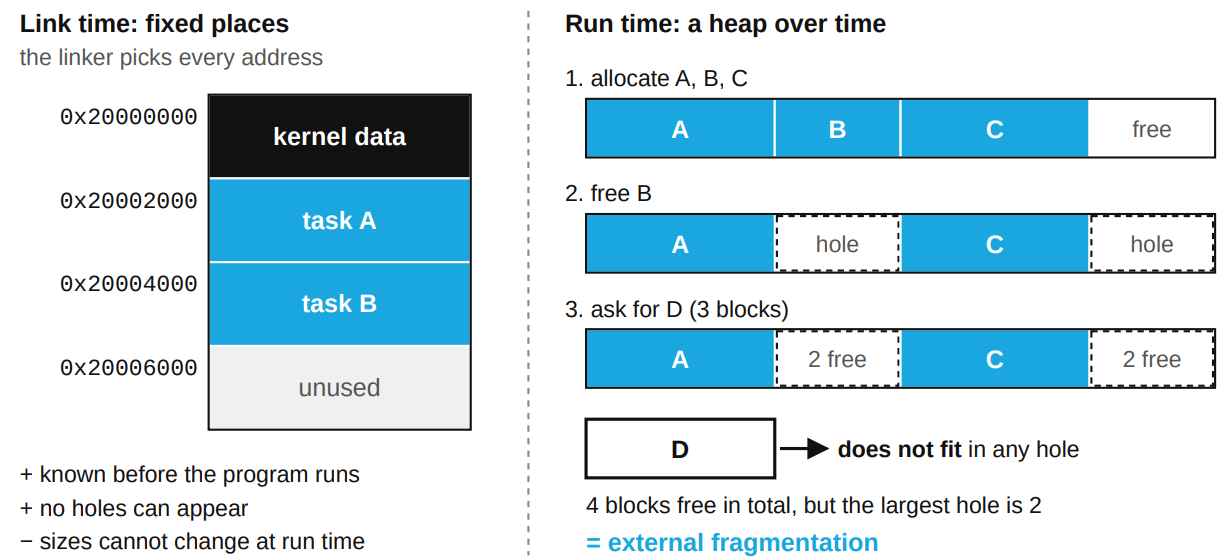
\includegraphics[width=0.7\textwidth]{contents/images/week-04/StaticVSDyn.png}
\end{figure}

For an embedded system dynamic allocation has two more problems: it can \textbf{fail at run time}, where nobody can read the error, and the time of a \texttt{malloc} depends on how many blocks it must search, so it is \textbf{not constant}, which is bad for deadlines. This course allocates \textbf{statically}; every partition of Unit 2 is fixed at link time.

\subsection{The Memory-Management Spectrum}

Memory management methods can be lined up by asking two questions: is the address changed before it reaches memory (\textbf{translation}), and does the hardware stop forbidden accesses (\textbf{protection})?

\begin{figure}[h]
    \centering
    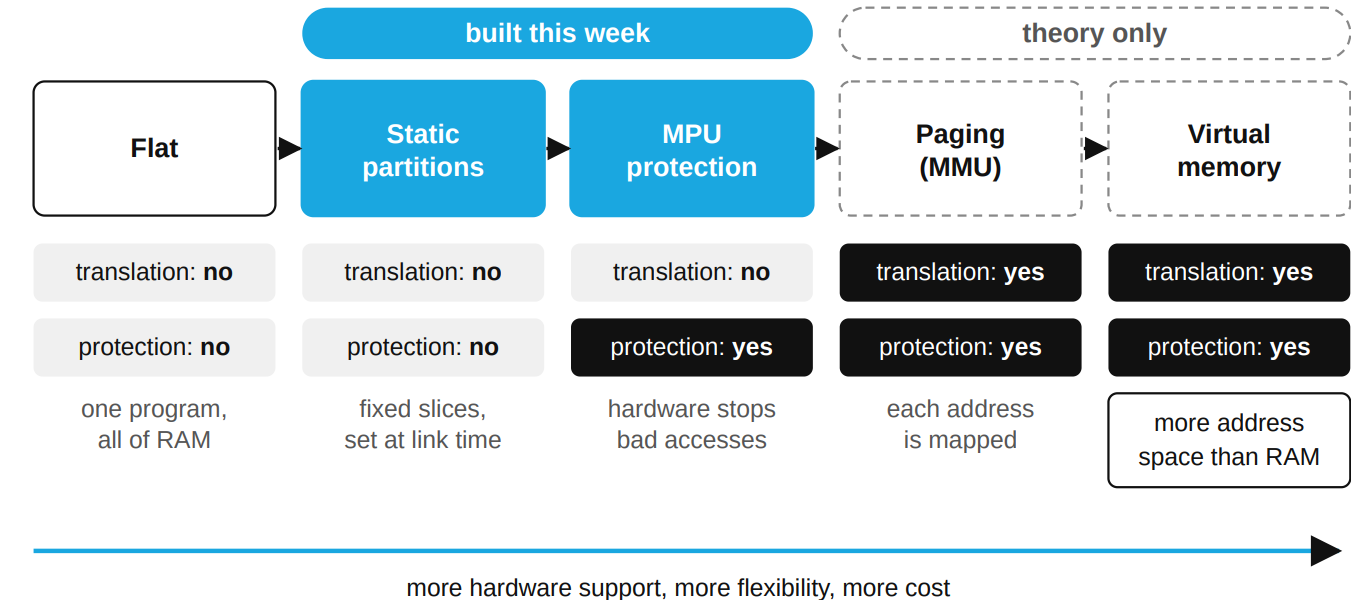
\includegraphics[width=0.7\textwidth]{contents/images/week-04/Covered_path.png}
\end{figure}

\begin{itemize}
    \item \textbf{Flat.} Everything shares all of RAM, with no translation and no protection. The starting code is here.
    \item \textbf{Static partitions.} Each task gets a fixed slice of RAM at link time: better placement, but still no protection (Unit 2).
    \item \textbf{MPU.} Hardware checks every access against a short list of allowed regions: protection without translation (Unit 3).
    \item \textbf{Paging with an MMU.} Hardware maps every address to a different physical one: translation and protection together (theory only).
    \item \textbf{Virtual memory.} Paging plus the disk, so that programs can use more memory than the RAM has (theory only).
\end{itemize}

Each step needs more hardware and buys more flexibility.

\subsection{A Rogue Task}

This is what ``no protection'' means in practice. With \texttt{make run DEMO=rogue}, right after its greeting, Task B executes this block of \texttt{src/task\_b.c}:

\begin{lstlisting}[language=C]
extern volatile uint32_t uptime_ms;     /* defined in another file; the linker gives its address */
printf( "B: writing to the kernel's uptime counter\n" );
uptime_ms = 0x12345678;                 /* a store into kernel memory */
\end{lstlisting}

\begin{lstlisting}
B: writing to the kernel's uptime counter
B: uptime 305420896 ms (second 1)
B: uptime 305421896 ms (second 2)
\end{lstlisting}

\texttt{0x12345678} is 305\,419\,896 in decimal and the kernel keeps counting from there, so one second later B reads 305\,420\,896 ms: Task B has \textbf{changed the kernel's clock}, for everyone. Nothing stopped it, because unprivileged mode blocks only some \textbf{instructions} (for example \texttt{msr} to CONTROL) and the system registers, not \textbf{ordinary loads and stores} to RAM. The lesson: a bug in one task can silently break the kernel or another task, and the damage shows up far from its cause. To stop it, the hardware must check every access.

\subsection{Paging: Pages, Frames and the MMU}

Paging is used by large operating systems (Linux, Windows, macOS). You do not build it, but you need it to understand what a microcontroller does differently.

A program uses \textbf{virtual addresses} (VA); the memory chips see \textbf{physical addresses} (PA). Paging maps one to the other:

\begin{itemize}
    \item The virtual space is cut into equal blocks called \textbf{pages} (often 4 KiB); physical memory is cut into \textbf{frames} of the same size. Any page can go in any frame.
    \item A \textbf{page table} says which frame holds each page, one table per \textbf{process}. Each entry has a \textbf{valid} bit (is the page in a frame at all?) and permission bits (read, write, execute, user or kernel only).
    \item The \textbf{MMU} (Memory Management Unit) is the hardware that translates \textbf{every} access and checks the permissions. It must be hardware: doing it in software for every load, store and fetch would be far too slow.
\end{itemize}

An address splits into a \textbf{page number} and an \textbf{offset}. Only the page number is translated; the offset is copied unchanged. With 4 KiB pages the offset is the low \textbf{12 bits} ($2^{12} = 4096$).

\textbf{A two-level walk.} With a 32-bit VA, one flat table indexed by 20 bits would need $2^{20}$ entries, that is 4 MiB \textbf{per process} even for a program using three pages. Real systems use \textbf{two levels}: a \textbf{page directory} whose entries point to second-level tables, with a register \textbf{PTBR} holding the directory address. The address is split into 10 bits of directory index, 10 bits of table index and 12 bits of offset, with 4-byte entries. Translate \texttt{VA = 0x00403007}:

\begin{lstlisting}
0x00403007 = 0000000001 | 0000000011 | 000000000111
             dir = 1       tbl = 3       offset = 7
\end{lstlisting}

\begin{figure}[h]
    \centering
    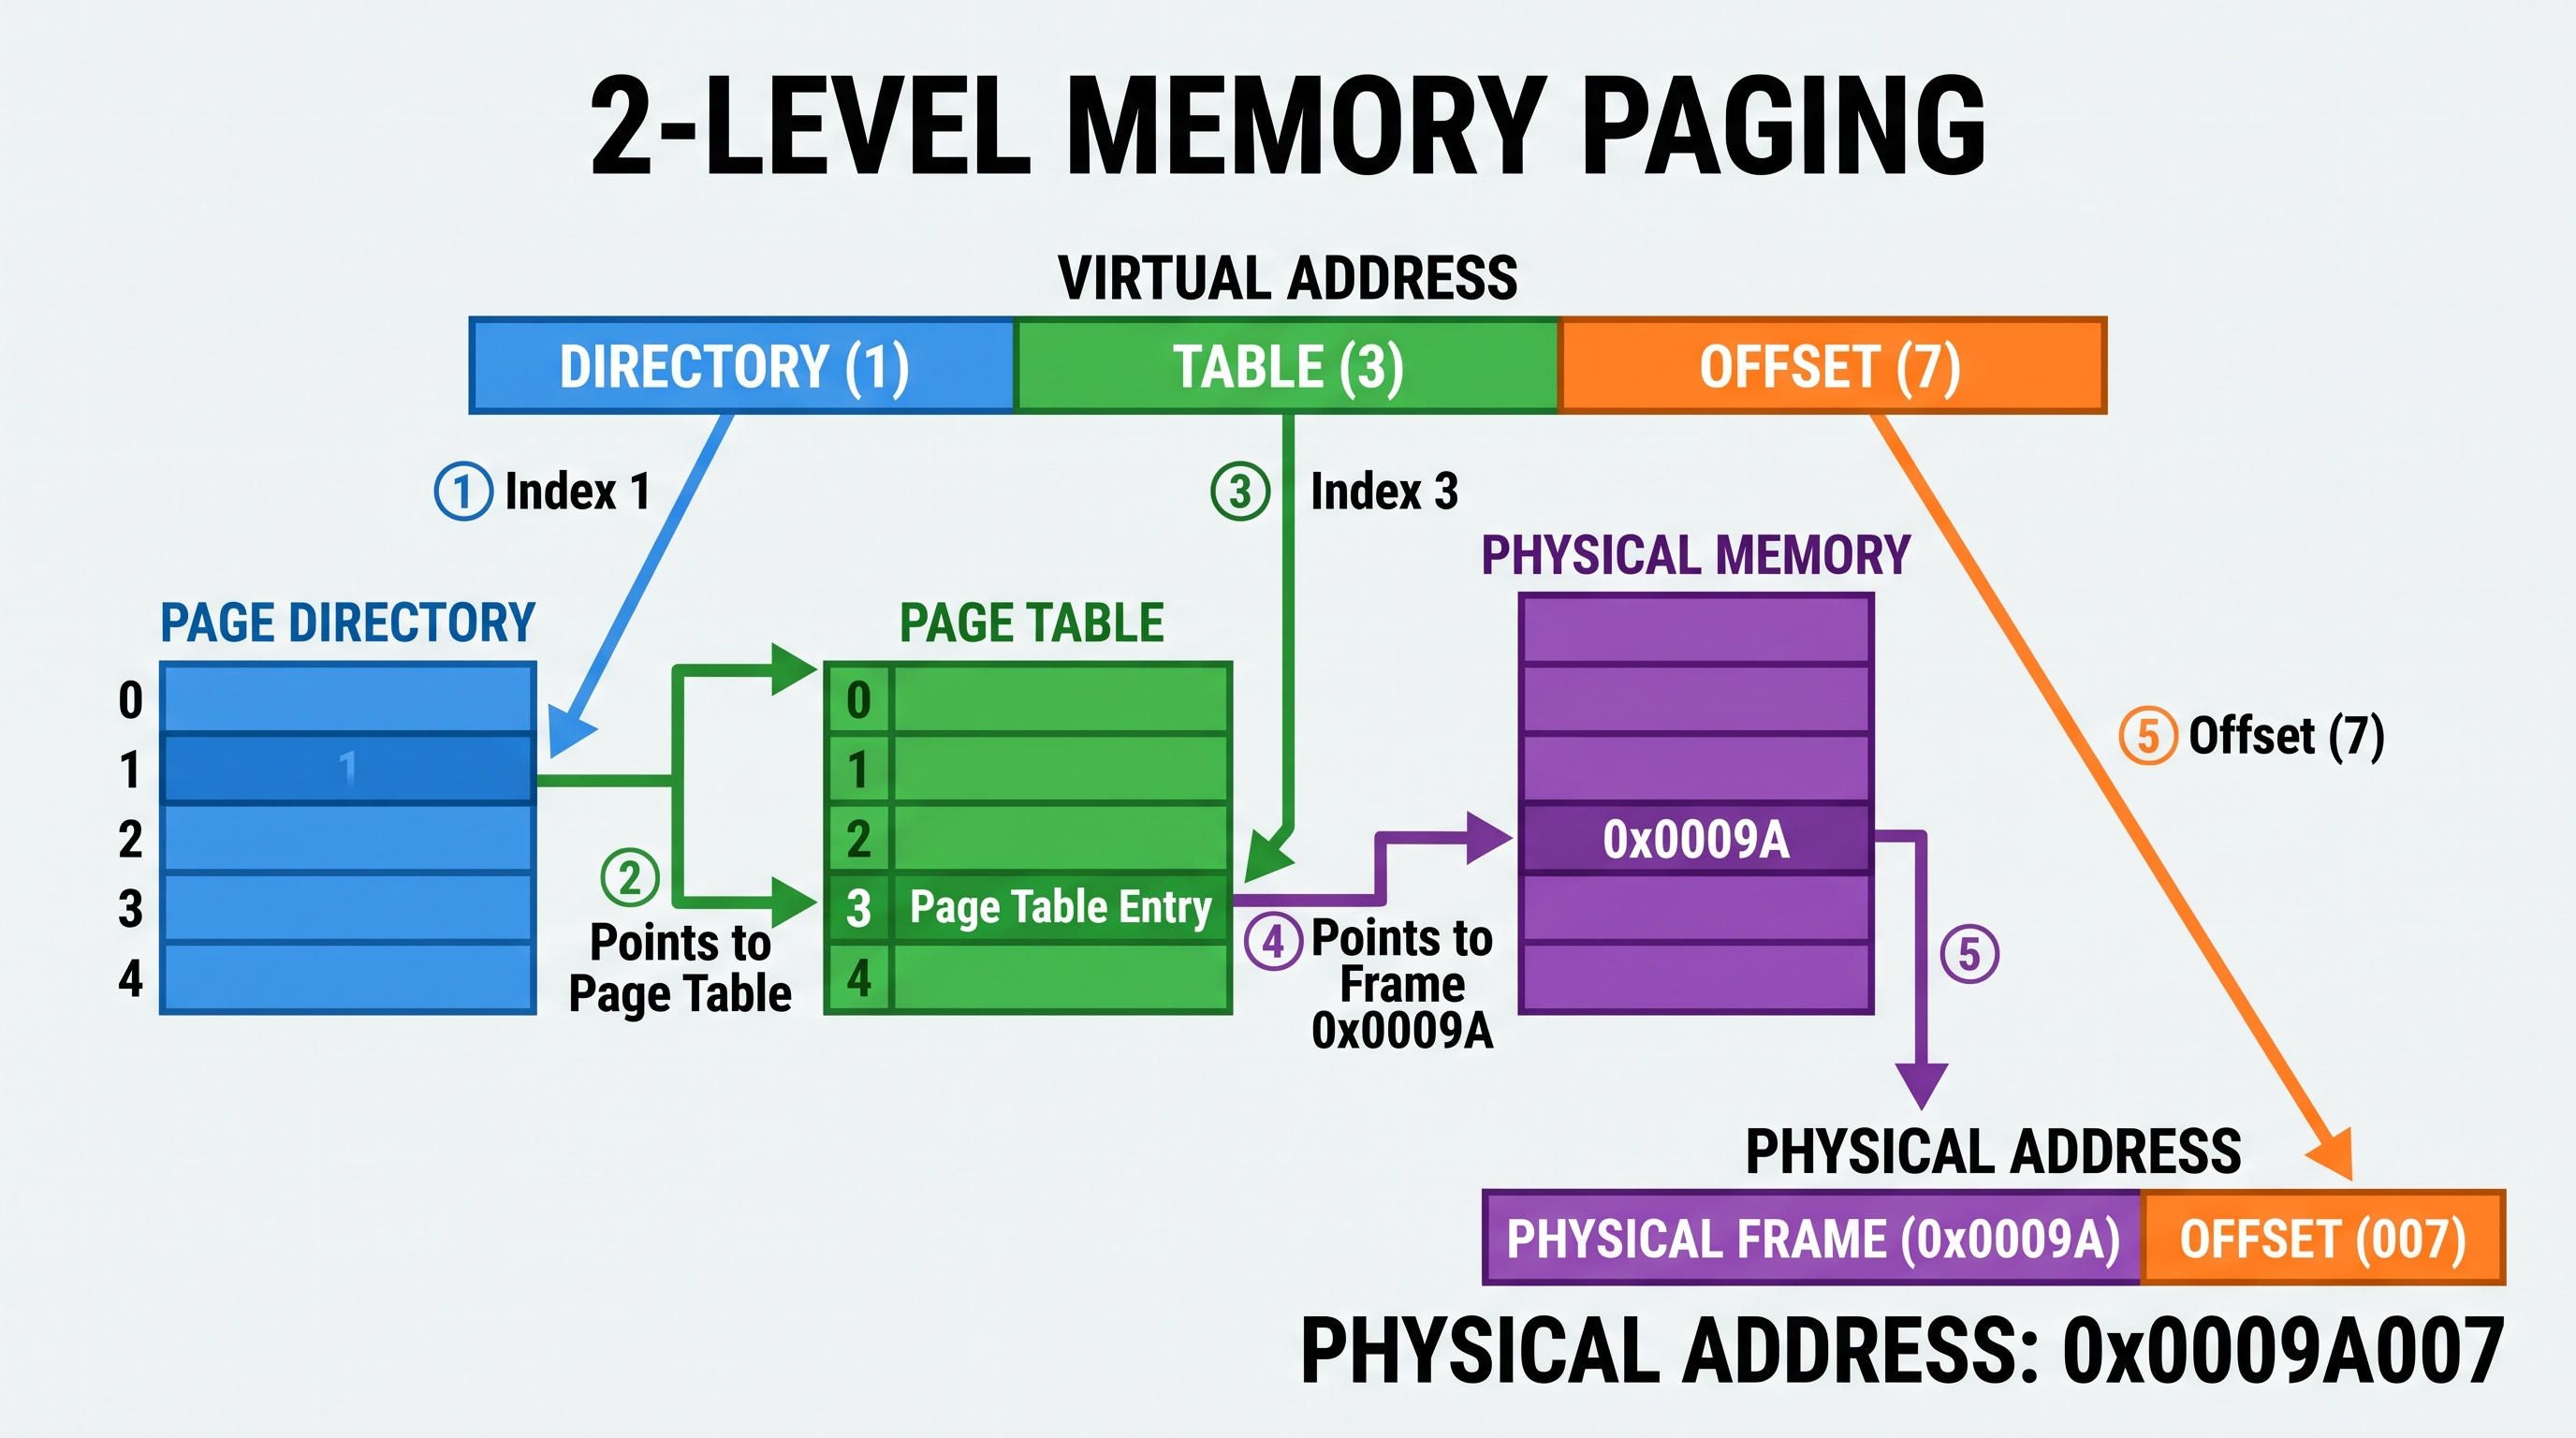
\includegraphics[width=0.7\textwidth]{contents/images/week-04/Paging.png}
\end{figure}

\begin{figure}[h]
    \centering
    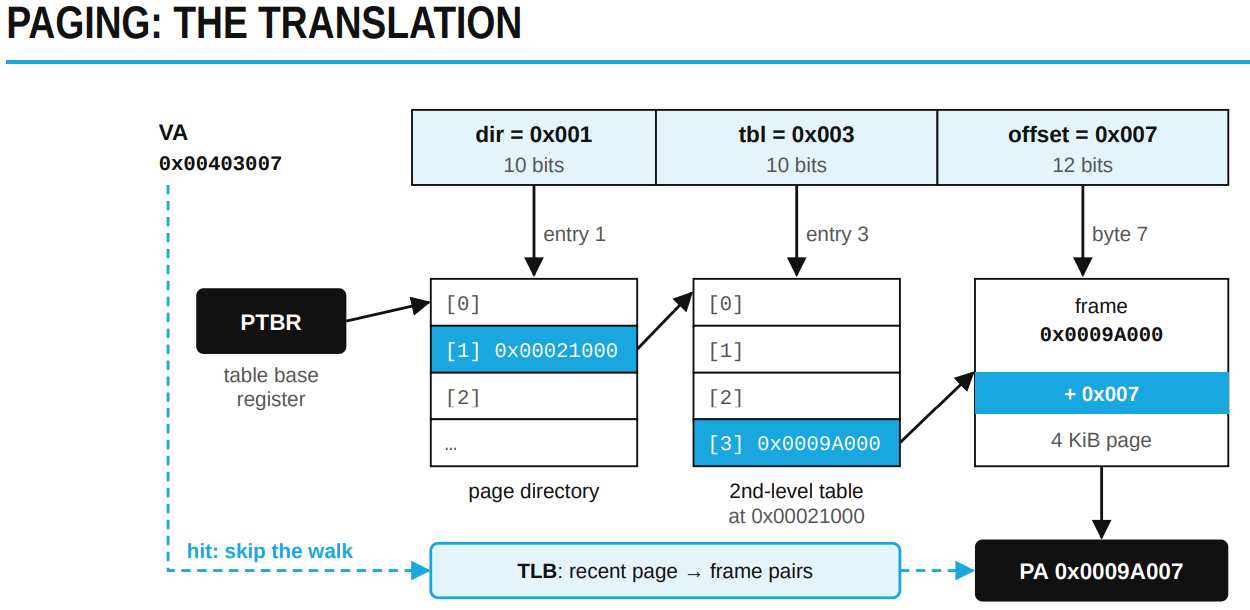
\includegraphics[width=0.7\textwidth]{contents/images/week-04/Paging_2.png}
\end{figure}

\begin{enumerate}
    \item Read directory entry 1, at \texttt{PTBR + 1 $\times$ 4}; say it holds the second-level table at \texttt{0x00021000}.
    \item Read entry 3 of that table, at \texttt{0x00021000 + 3 $\times$ 4 = 0x0002100C}; say it holds frame \texttt{0x0009A000}, valid.
    \item PA = frame + offset = \texttt{0x0009A000 + 0x007 = 0x0009A007}.
\end{enumerate}

Two levels pay off because a second-level table exists \textbf{only where memory is used}: a small process needs one directory (4 KiB) and a few tables instead of a 4 MiB table made mostly of invalid entries.

\subsection{The TLB and the Cost of Paging}

The walk costs \textbf{two extra memory reads} per access, which would make memory three times slower. The \textbf{TLB} (Translation Lookaside Buffer) is a small, fast cache inside the MMU that keeps recent translations (page number $\rightarrow$ frame, plus permissions). On a \textbf{hit} the frame comes straight from the TLB; on a \textbf{miss} the MMU walks the tables and stores the result. Programs reuse the same few pages (loop code, stack, current array), so most accesses hit. Since it is a cache, the OS must \textbf{flush} the stale entries when it changes a page table or switches process, otherwise a process could reach the previous one's frames.

\textbf{Effective access time (EAT).} It is the average time of one access, translation included. With \texttt{m} the time of one memory access and \texttt{h} the \textbf{hit ratio}, a hit costs \texttt{m} and, with a two-level table, a miss costs \texttt{3m} (directory read, table read, the access itself):

\begin{lstlisting}
EAT = h * m + (1 - h) * 3m = m * (3 - 2h)
\end{lstlisting}

Each miss adds \texttt{2m}, so the \textbf{slowdown} over plain memory is $2 \times (1 - h)$: 1\% of misses makes memory 2\% slower. With \texttt{m = 10 ns} (a hit costs 10 ns, a miss 30 ns):

\begin{lstlisting}
no TLB      EAT = 30 ns                                  3x slower
h = 0.80    EAT = 0.80 * 10 + 0.20 * 30 = 14.0 ns        +40%
h = 0.99    EAT = 0.99 * 10 + 0.01 * 30 = 10.2 ns        +2%
\end{lstlisting}

\begin{figure}[h]
    \centering
    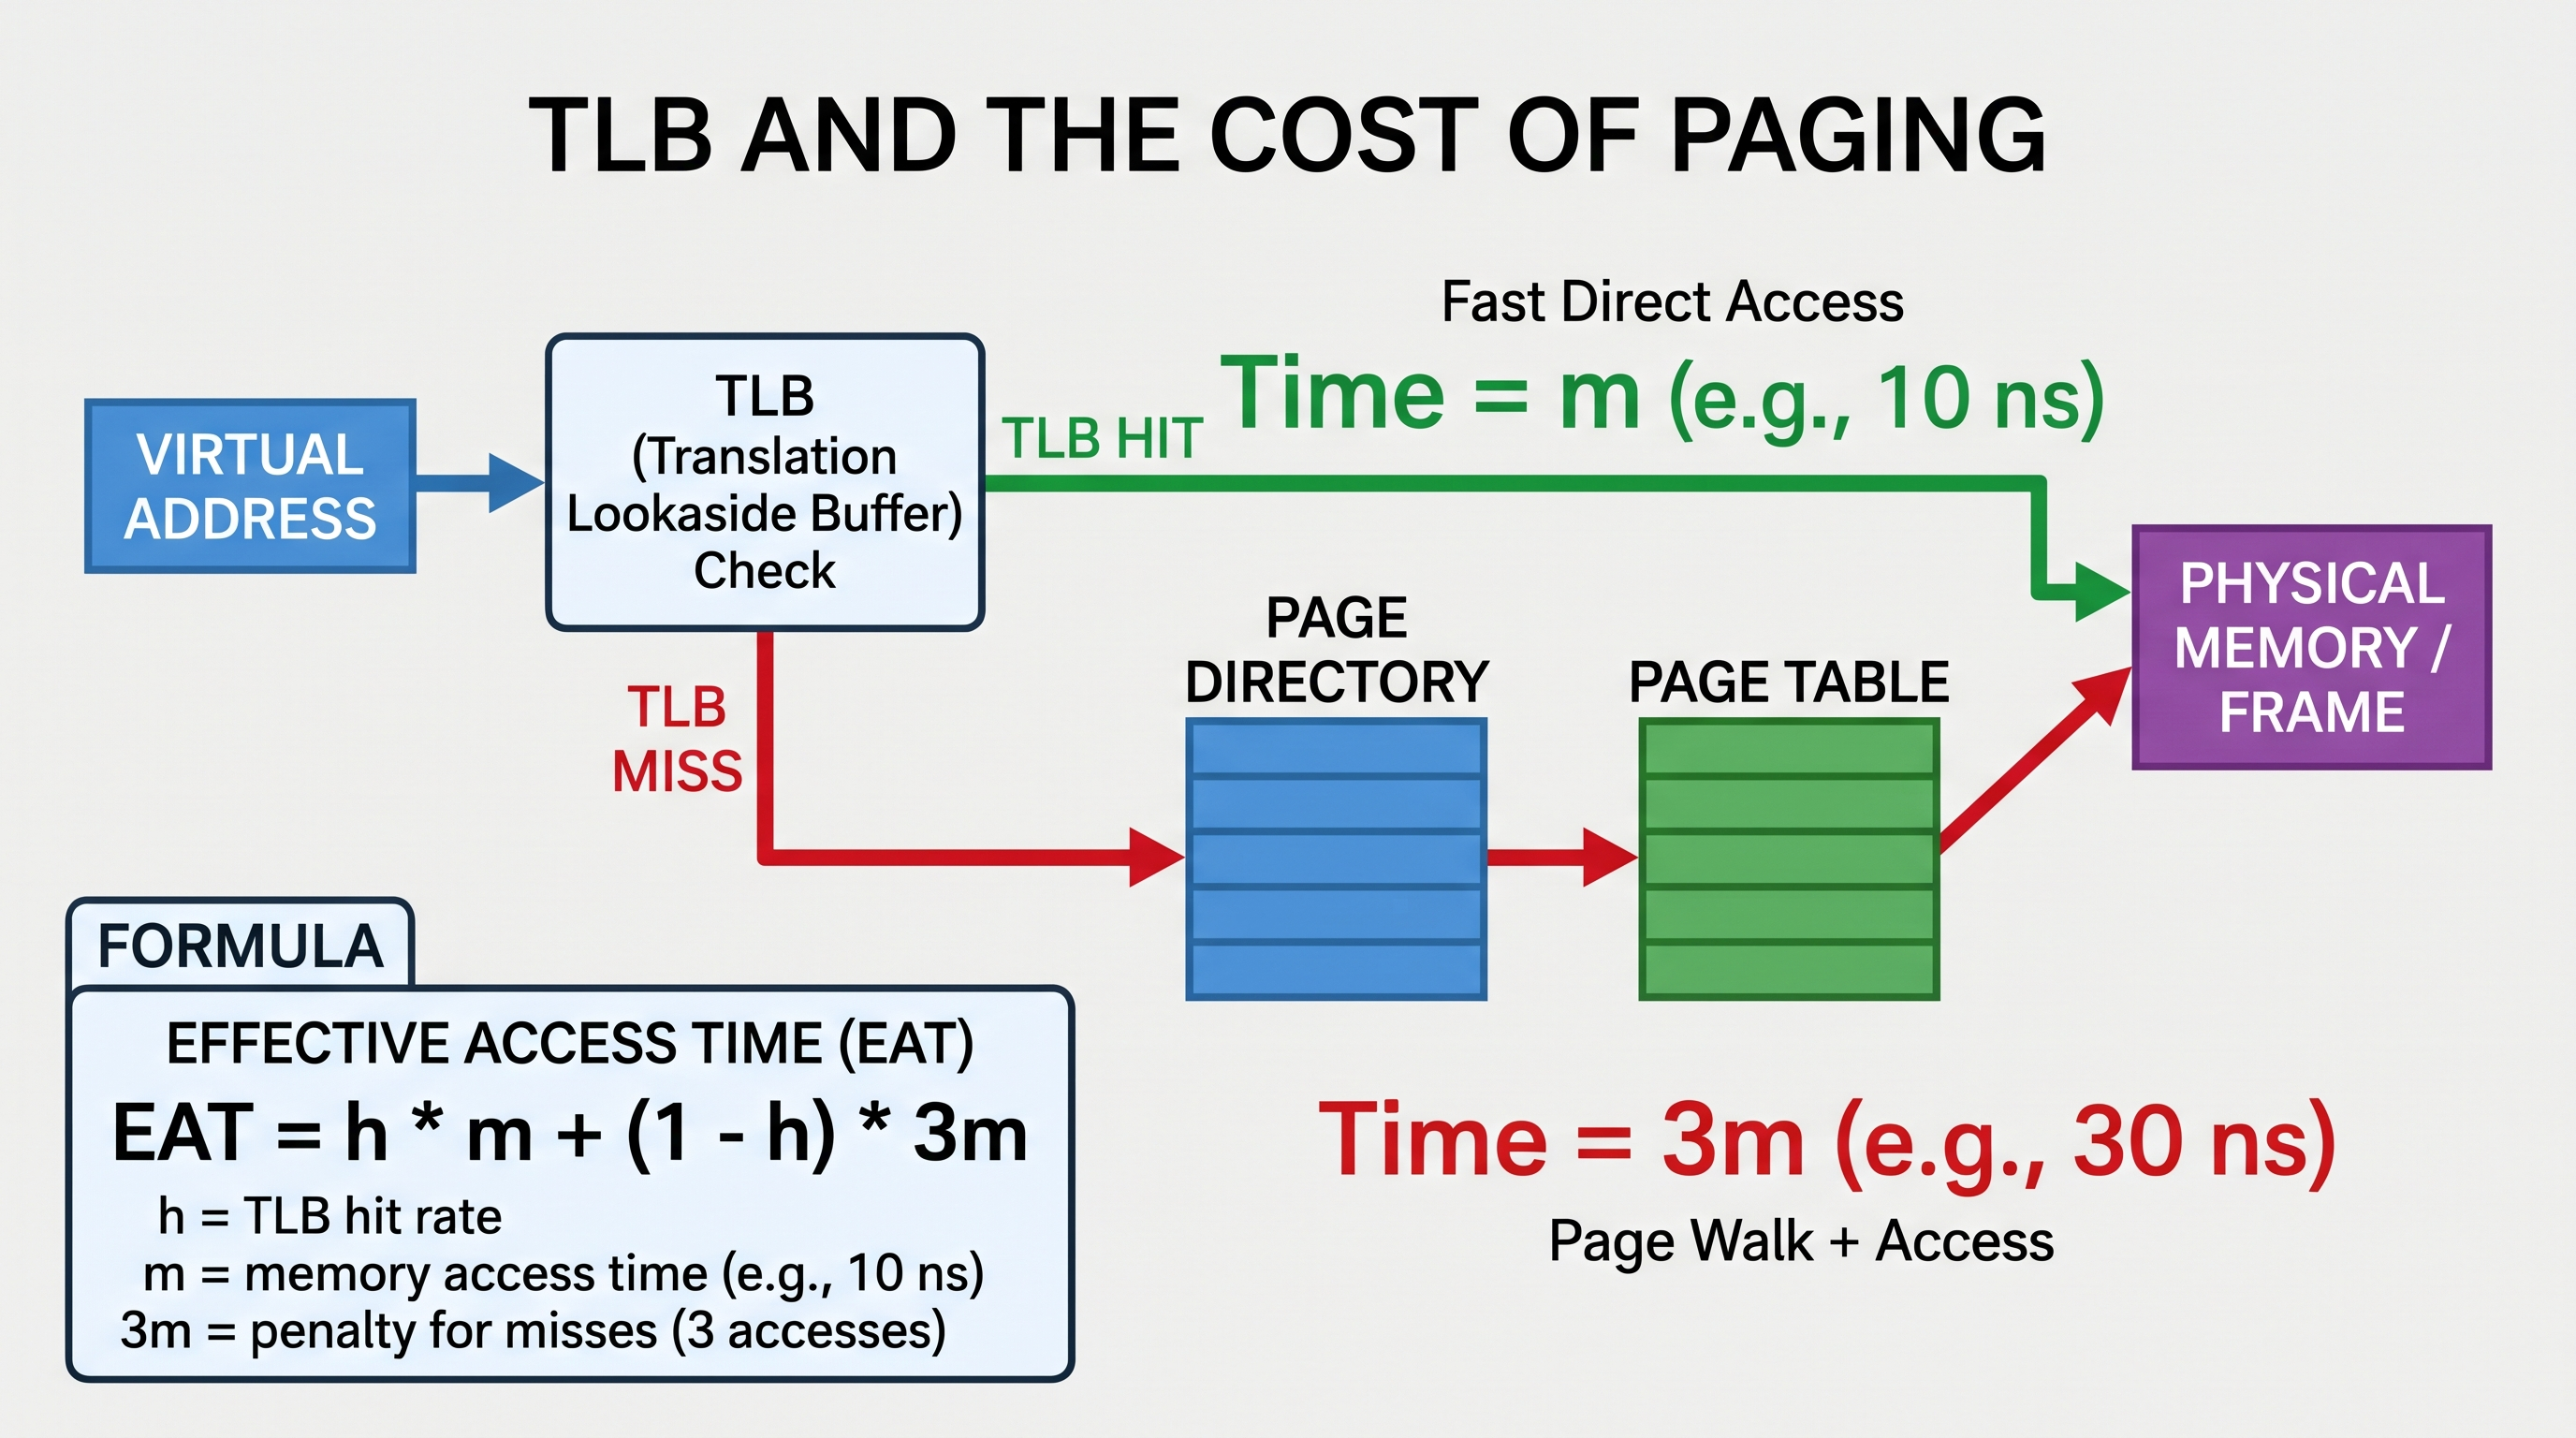
\includegraphics[width=0.7\textwidth]{contents/images/week-04/TLB.png}
\end{figure}

The misses, not the hits, set the cost, so \texttt{h} must be close to 1. Useful rules:

\begin{itemize}
    \item \textbf{How high must \texttt{h} be?} For a slowdown of at most \texttt{s}: $2 \times (1 - h) \le s$, so $h \ge 1 - s/2$ (at most 5\% needs $h \ge 0.975$).
    \item \textbf{Deeper tables.} 64-bit systems use \textbf{four} levels: a miss costs \texttt{5m} and the slowdown is $4 \times (1 - h)$, twice as much for the same \texttt{h}.
    \item \textbf{Why \texttt{h} is high: locality.} A loop reading an array misses once per 4 KiB page and hits on the other 1023 words of that page.
    \item \textbf{TLB reach.} 64 entries of 4 KiB cover $64 \times 4$ KiB = \textbf{256 KiB}; a program that jumps at random over 1 GiB misses almost always. Bigger pages (2 MiB) increase the reach.
    \item \textbf{After a flush} the TLB is empty and the first accesses miss: for a real-time task this is \textbf{jitter}, since access time depends on what the TLB happens to hold.
\end{itemize}

\textbf{Exercise.} With \texttt{m = 50 ns} and a two-level table: with no TLB the EAT is 150 ns (3x slower); with \texttt{h = 0.90} it is $0.90 \times 50 + 0.10 \times 150 = 60$ ns (+20\%); with \texttt{h = 0.98} it is 52 ns (+4\%); for a slowdown of at most 10\% we need $h \ge 0.95$. With four levels and \texttt{h = 0.98} a miss costs 250 ns, so EAT $= 0.98 \times 50 + 0.02 \times 250 = 54$ ns (+8\%). A loop that reads a 64 KiB array of 32-bit words once, with 4 KiB pages and an empty TLB, takes 16 misses out of 16\,384 accesses, so $h = 1 - 16/16\,384 \approx 0.999$.

\subsection{Page Faults and Virtual Memory}
If the walk finds an entry with the valid bit clear, or the access breaks its permissions (a write to a read-only page, user code touching a kernel page), the MMU raises a \textbf{page fault}, an exception that records the address wanted:

\begin{enumerate}
    \item If the address is not part of the program or the access is not allowed, the OS \textbf{kills the process}.
    \item If the address is legal but the page is not in RAM, the OS finds a free frame, reads the page from disk, fills the table entry and sets the valid bit.
    \item The handler returns and the hardware \textbf{restarts the faulting instruction}. It is restarted, not skipped, because its load or store never happened; restarting makes the fault invisible to the program.
\end{enumerate}

\begin{figure}[h]
    \centering
    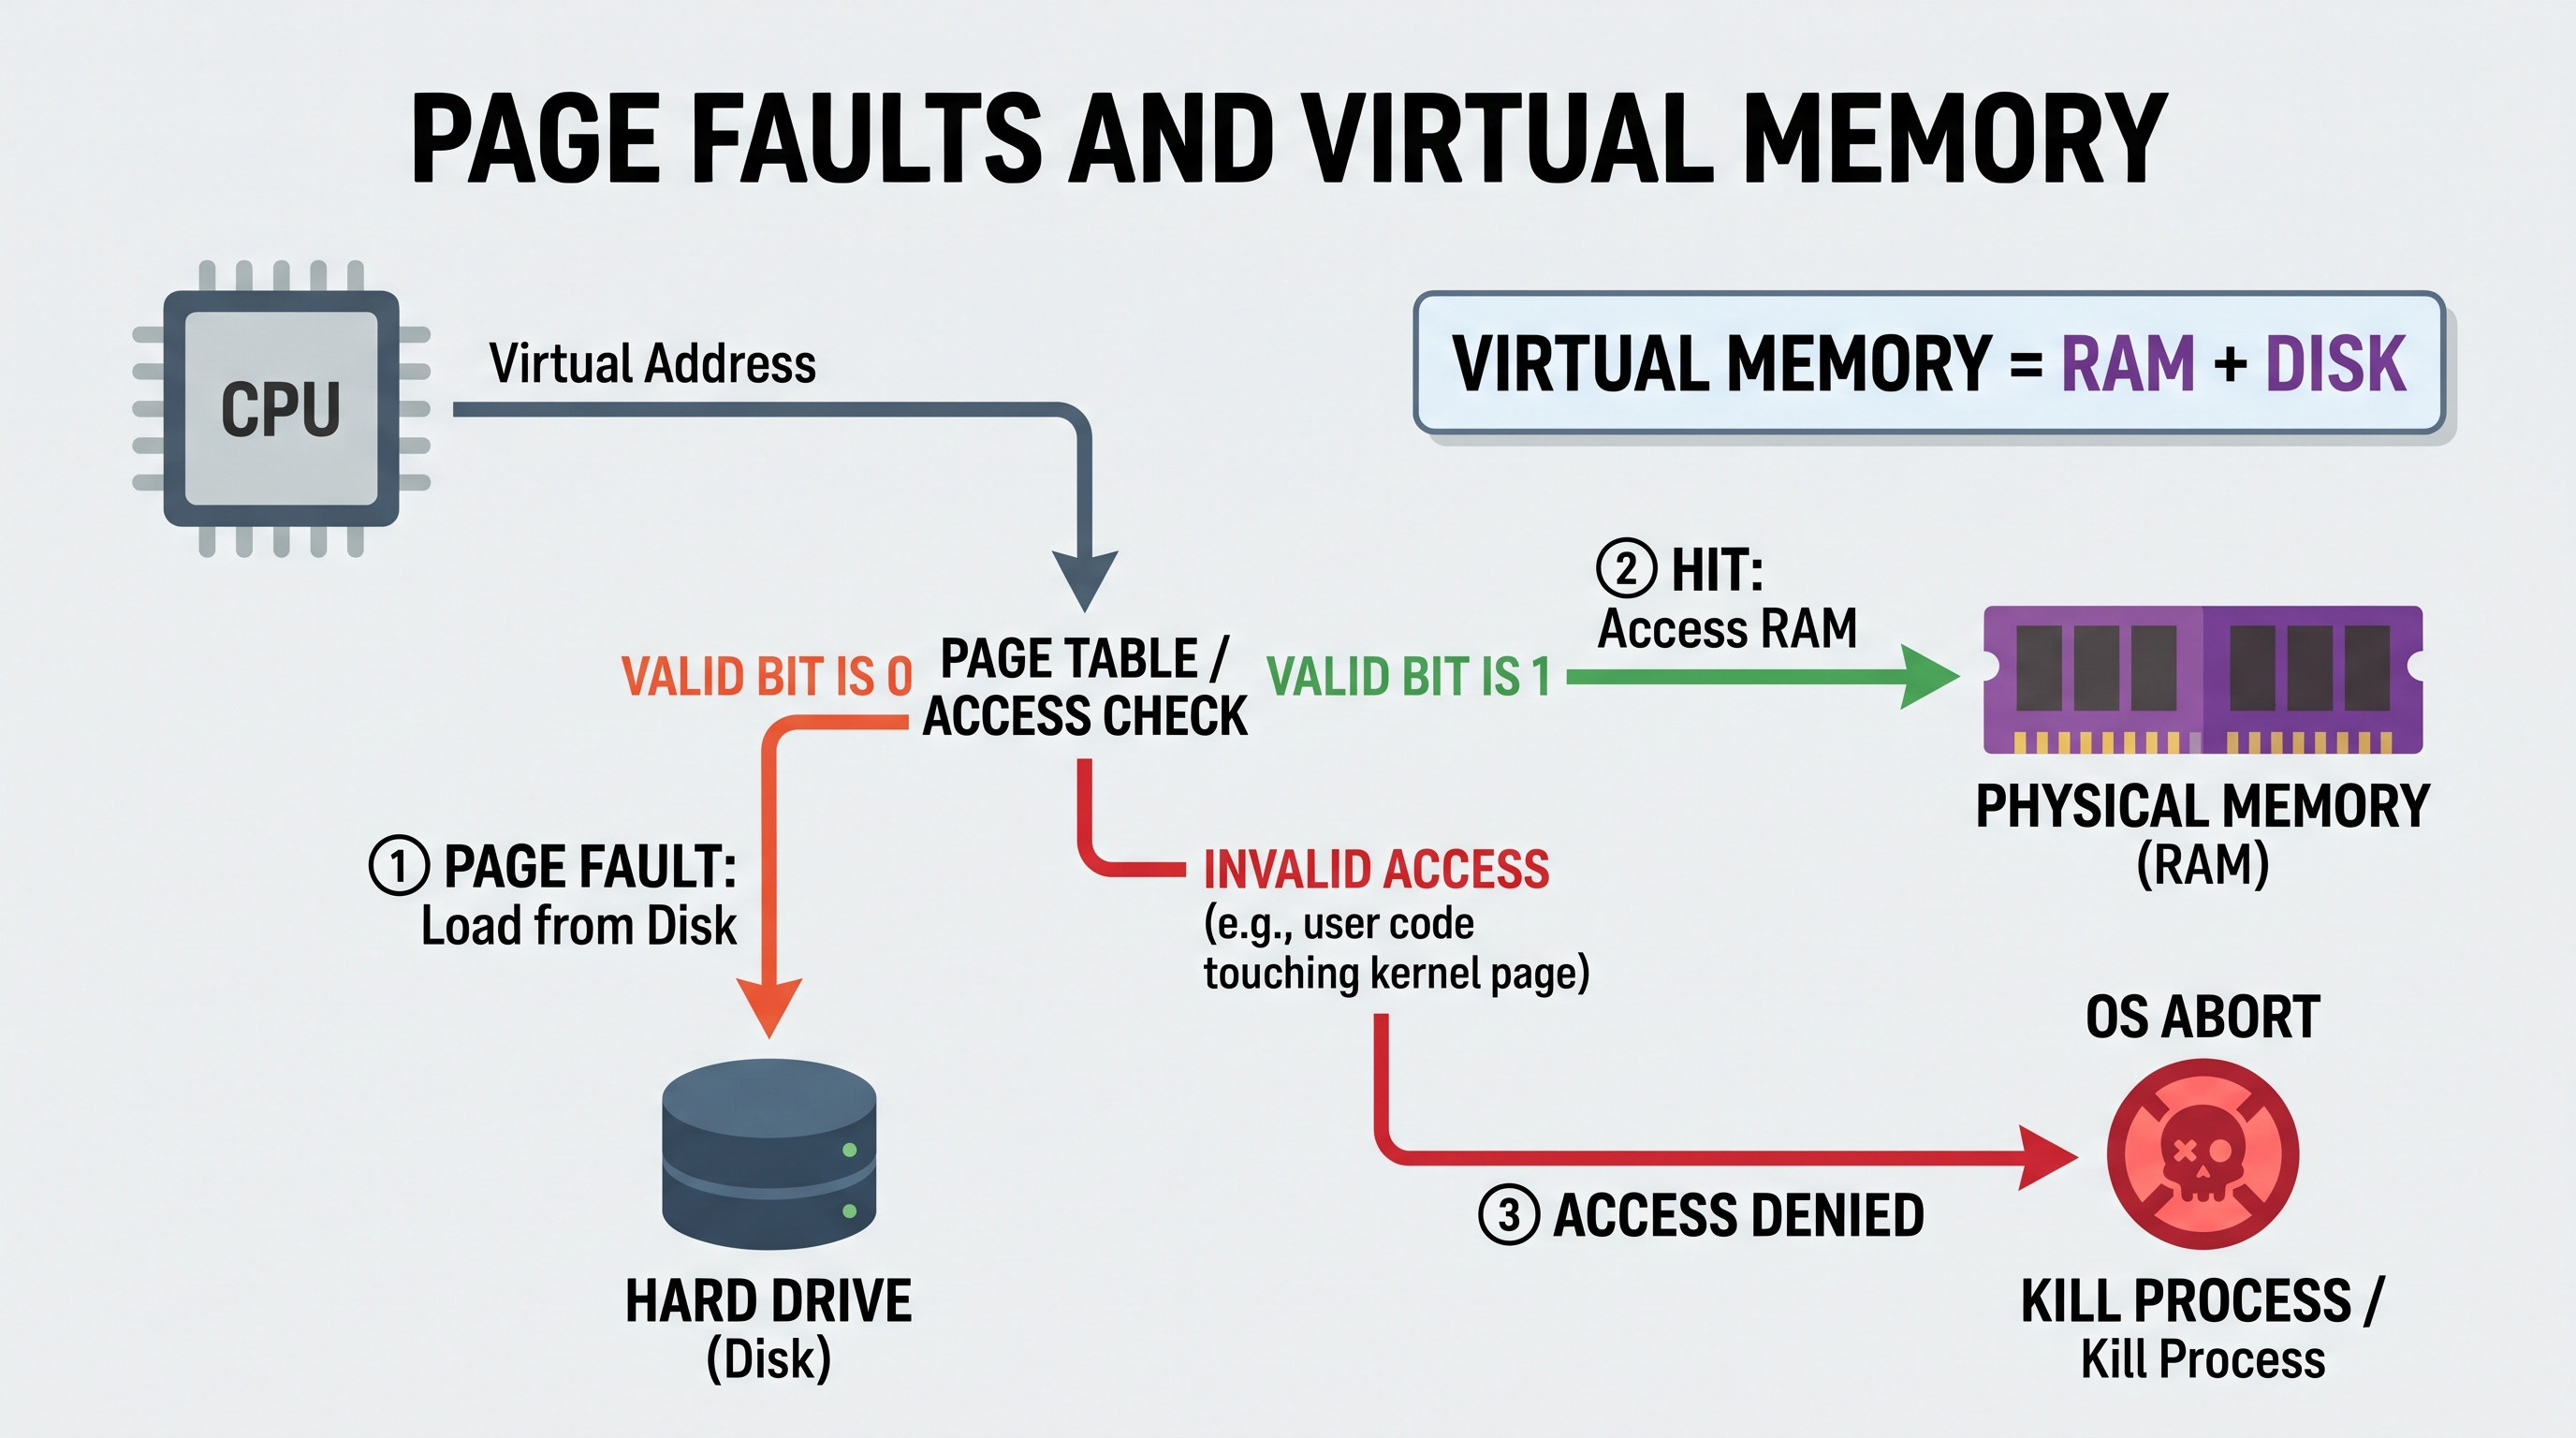
\includegraphics[width=0.7\textwidth]{contents/images/week-04/Page_Faults.png}
    \caption{Page Hits and Faults}
\end{figure}

\textbf{Cost.} A fault that reads the disk costs \textbf{milliseconds}, against nanoseconds for an access. With \texttt{p} the page-fault rate, $\text{EAT} = (1 - p) \times m + p \times \text{(service time)}$. With \texttt{m = 200 ns} and a service time of 8 ms: $p = 1/1000$ gives about 8.2 $\mu$s, \textbf{forty times slower}; to lose at most 10\%, $p \le 2.5 \times 10^{-6}$, fewer than \textbf{one access in 400\,000}. Virtual memory works only because locality makes faults so rare, and one fault stops the program for milliseconds at an unpredictable moment: a real-time system cannot accept that.

\textbf{Virtual memory} is paging plus the disk, and it gives two things:
\begin{itemize}
    \item \textbf{Isolation.} Each process has its own page table, so the same virtual address lands in different frames for different processes. A process cannot even \textbf{name} another process's memory: its own table translates every address into its own frames, or into a page fault.
    \item \textbf{More than RAM.} Pages not in use wait on disk and a page fault brings them back, so programs together can use more memory than the RAM has, as long as the pages in use at any moment fit.
\end{itemize}

\begin{figure}[h]
    \centering
    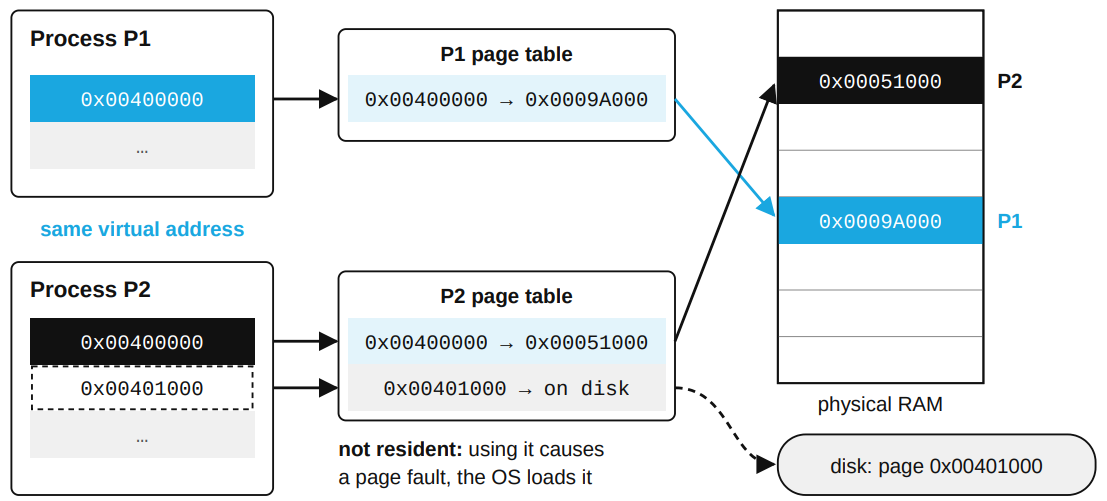
\includegraphics[width=0.7\textwidth]{contents/images/week-04/Virtual_Memory.png}
    \caption{Memory Virtualitation}
\end{figure}

This answers the fourth job of the OS, and protection in the strongest way, but it needs an MMU, page tables in RAM and a disk.

\subsection{MPU versus MMU}

A microcontroller has neither page tables nor a disk. The Cortex-M3 has an \textbf{MPU} (Memory Protection Unit): a short list of \textbf{regions}, each with a start address, a size and \textbf{permissions} (who may read, write, execute, separately for privileged and unprivileged code).

\begin{itemize}
    \item On \textbf{every} load, store and fetch the MPU checks the address against the regions. If allowed, the access goes on at the \textbf{same} address; otherwise it is stopped (the store writes nothing, the load reads nothing) and the CPU raises a \textbf{MemManage} fault.
    \item There is \textbf{no translation}: every task sees real physical addresses, and the MPU only answers ``may this code touch this address?''
\end{itemize}

\begin{figure}[h]
    \centering
    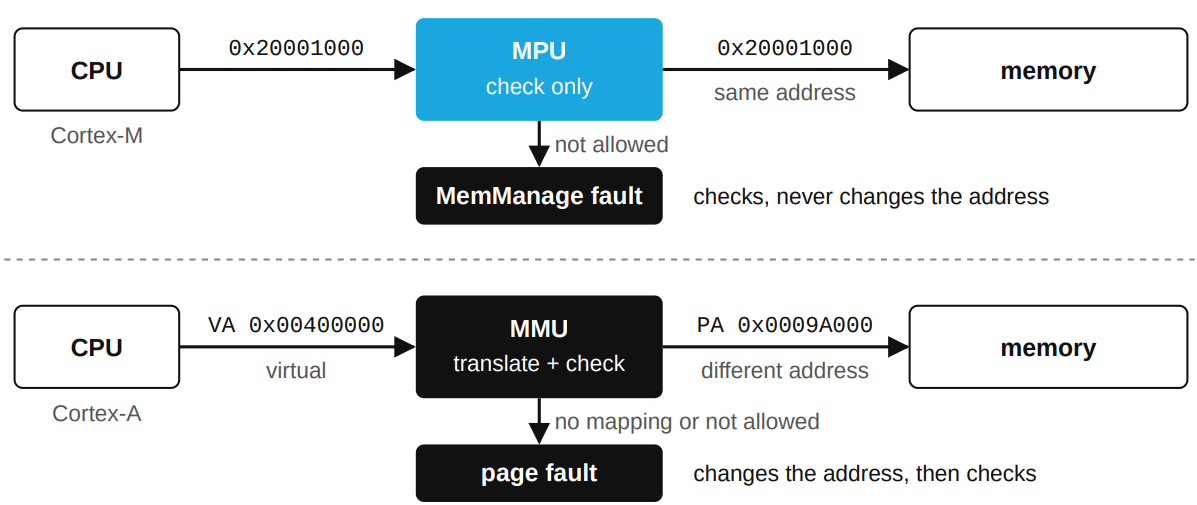
\includegraphics[width=0.7\textwidth]{contents/images/week-04/MPU_vs_MMU.png}
\end{figure}

Microcontroller cores (Cortex-M) have an MPU; application cores (Cortex-A, in phones and Linux boards) have an MMU, which turns VA into PA or raises a page fault. The MPU of this board is \textbf{off} after reset, which is why the rogue write went through; you turn it on in Unit 3.

Why does a microcontroller not have an MMU?
\begin{itemize}
    \item \textbf{Cost and area:} an MMU needs page tables in RAM, a hardware walker and a TLB; an MPU is a handful of registers.
    \item \textbf{Power:} no walks and no extra reads on a miss.
    \item \textbf{Determinism:} a TLB miss makes an access slower by an unpredictable amount; an MPU check takes the same time every time, which matters for deadlines.
    \item \textbf{No disk} to swap to, and \textbf{small, fixed programs} for which regions decided at build time are enough.
\end{itemize}

What you give up is translation: every task must be placed at its own real address by the linker (Unit 2), and the MPU has only a few regions with rules on size and alignment (Unit 3).

\subsection{A Bad Pointer}

The last demo shows a different leak. With \texttt{DEMO=badptr}, Task B asks the \textbf{kernel} to touch kernel memory, by passing a kernel address to the system call of Week 3 (``send these \texttt{len} bytes from \texttt{buf} to the console''):

\begin{lstlisting}
int r = sys_write( (const char *) &uptime_ms, 16 );
printf( "\nB: sys_write returned %d\n", r );
\end{lstlisting}

\begin{lstlisting}
B: hello from task B
^K^@^@line 2)
A: u
B: sys_write returned 16
\end{lstlisting}

The 16 bytes start at \texttt{uptime\_ms}: its 4 bytes hold \texttt{0x00000BB8} (3000 ms), stored low byte first (\texttt{B8 0B 00 00}), not printable, so the terminal shows odd symbols (\texttt{\^{}K\^{}@\^{}@}). The next 12 bytes are the start of \texttt{tx\_buf}, still holding old text of Task A. Task B has read the kernel's private data \textbf{through the kernel}: \texttt{sys\_write} returns 16 because the kernel, running in the SVC handler, \textbf{privileged}, reaches any address it is given.

The consequence for Unit 3: an MPU that restricts only unprivileged code would \textbf{not} stop this leak, because the reads are the kernel's. The kernel must check the pointer itself before using it.

\subsection{End of Unit 1}

\begin{itemize}
    \item An OS manages memory to \textbf{place} it, \textbf{share} it, \textbf{protect} it, and to run more programs than fit. The starting code does placement only, per variable, with no border between kernel and tasks.
    \item This course allocates \textbf{statically}, at link time: dynamic allocation fragments the heap, can fail at run time and takes variable time.
    \item \textbf{Paging:} the MMU translates page to frame through page tables, the TLB caches translations, a page fault restarts the instruction once the page is in. \textbf{Virtual memory} adds isolation and the disk.
    \item \textbf{Cost of paging:} $\text{EAT} = h \times m + (1 - h) \times 3m$ with two levels; \texttt{h} must be close to 1 and page faults extremely rare.
    \item An \textbf{MPU} checks every access against regions, with no translation: cheap, low-power, predictable. The Cortex-M3 has one, switched off. Without it, \texttt{DEMO=rogue} changes the kernel's clock and \texttt{DEMO=badptr} leaks kernel bytes through a system call.
\end{itemize}


\section{Unit 2: Task Partitions}

\subsection{The Target: One Slice of RAM per Task}

A \textbf{partition} is a slice of RAM that belongs to a single task and holds only its stack and variables. FLASH holds the code, the read-only data and the initial values of the task variables. The goal is this RAM layout:

\begin{lstlisting}
0x20000000   Task A partition (4 KB): [ stack 1 KB | A's variables | padding ]
0x20001000   Task B partition (4 KB): [ stack 1 KB | B's variables | padding ]
0x20002000   kernel .data and .bss
   ...       (free RAM)
   top       kernel stack
\end{lstlisting}

The partitions follow five rules:

\begin{itemize}
    \item \textbf{Fixed.} The linker chooses them at link time (static allocation of Unit 1): no task is created, grown or moved at run time.
    \item \textbf{4 KB, aligned to 4 KB.} The size is a power of two and each start is a multiple of 4096 (\texttt{0x20000000}, \texttt{0x20001000}), which is exactly the shape the MPU of Unit 3 can protect. The price is waste: a task that needs 1.1 KB still gets 4 KB.
    \item \textbf{RAM only.} Code and read-only data (\texttt{.text}, \texttt{.rodata}, string literals) stay in FLASH, \textbf{shared} by the kernel and both tasks: one copy of \texttt{printf} serves everybody.
    \item \textbf{Stack at the bottom.} The stack takes the lowest 1 KB and the variables sit above it. Since the stack grows \textbf{down}, an overflow leaves the partition immediately, below its start, where Unit 3 will make it fault. With the stack at the top, an overflow would silently overwrite the task's own variables, and no protection hardware could tell that write from a legitimate one.
    \item \textbf{The kernel keeps the rest:} its \texttt{.data} and \texttt{.bss} come after the partitions and its stack stays at the top of RAM.
\end{itemize}

\subsection{Linker Tools You Need}

An \textbf{output section} has two addresses: the \textbf{run address} (VMA), where the code uses it, and the \textbf{load address} (LMA), where its bytes are stored in the image. They are usually equal, but not for \texttt{.data}. The partition block uses:

\begin{lstlisting}
.task_a_data : { ... } > RAM AT > FLASH          /* runs in RAM, initial bytes stored in FLASH */
_task_a_data_load = LOADADDR(.task_a_data);      /* the FLASH address of those bytes */
.task_a_stack ALIGN(ORIGIN(RAM), 4096) (NOLOAD) : { ... } > RAM
*task_a.o(.data .data.* .bss .bss.* COMMON)      /* these input sections, from task_a.o only */
\end{lstlisting}

\begin{itemize}
    \item \textbf{\texttt{> RAM AT > FLASH}} (as for Week 2's \texttt{.data}): variables run in RAM but their initial bytes are stored in FLASH, which keeps its content without power. Somebody must copy them before use: \texttt{Reset\_Handler} does it for the kernel; for a partition the kernel does it just before the task's first run.
    \item \textbf{\texttt{(NOLOAD)}} reserves addresses but stores \textbf{nothing} in the image: right for a stack or padding.
    \item \textbf{\texttt{ALIGN(x, 4096)}} rounds \texttt{x} \textbf{up} to a multiple of 4096; before the colon it sets the section's start. For the first partition we use \texttt{ALIGN(ORIGIN(RAM), 4096)} because right after \texttt{.text} the location counter \texttt{.} is still a FLASH address; for B, \texttt{.} is already in RAM, so \texttt{ALIGN(4096)} is enough.
    \item \textbf{\texttt{. = start + 4096}} jumps to the end of the partition, whatever was placed before.
    \item \textbf{File patterns.} \texttt{*task\_a.o(...)} takes the variables of \texttt{src/task\_a.c} only, so the source needs no special marking. \texttt{.bss} is put in the same loaded section as \texttt{.data}: its zeros are stored in FLASH too (4 bytes here), and a single copy loop initializes every task variable.
    \item \textbf{The first match wins.} Every input section is placed by the first rule that matches it, so the partition rules must come \textbf{before} the kernel's generic \texttt{*(.data*)} and \texttt{*(.bss*)}, otherwise the task variables would stay in kernel RAM.
    \item \textbf{Exported symbols and \texttt{ASSERT}} (Week 2). The prepared kernel already uses six symbols per task (\texttt{\_task\_X\_part\_start}, \texttt{\_part\_end}, \texttt{\_stack\_top}, \texttt{\_data\_start}, \texttt{\_data\_end}, \texttt{\_data\_load}, with \texttt{X} = \texttt{a} or \texttt{b}); your edit only \textbf{re-points} them. \texttt{ASSERT(cond, "msg")} fails the link if \texttt{cond} is false, so a task that grows too big is caught at build time.
\end{itemize}

\subsection{The Partition Block}

All edits are in \texttt{scripts/mps2\_m3.ld} (in your copy, \texttt{week-04/base/scripts/}), three in total:

\begin{enumerate}
    \item After the line \texttt{TASK\_STACK\_SIZE = 0x400;} add \texttt{PART\_SIZE = 0x1000;} (4 KB per partition).
    \item Near the end, \textbf{delete} everything from the comment \texttt{/* >>> UNIT 2: delete from this comment down to \_task\_b\_data\_load. <<<} down to the line \texttt{\_task\_b\_data\_load = LOADADDR(.data);} included: the flat \texttt{.task\_stacks} section and the empty data symbols. Keep \texttt{\_\_StackLimit} and the \texttt{ASSERT} after it, which protect the kernel stack.
    \item Replace the comment \texttt{/* >>> UNIT 2: paste the task partitions here, before .data (see the slides). <<< */}, right after \texttt{.text} and before \texttt{\_sidata = LOADADDR(.data);}, with the partition of A followed by that of B.
\end{enumerate}

Task A's partition is made of three output sections:

\begin{lstlisting}
    .task_a_stack ALIGN(ORIGIN(RAM), 4096) (NOLOAD) : {
        _task_a_part_start = .;            /* partition start = stack bottom */
        . = . + TASK_STACK_SIZE;           /* reserve the 1 KB stack */
        _task_a_stack_top = .;             /* the stack grows down from here */
    } > RAM
    .task_a_data : {
        . = ALIGN(4);
        _task_a_data_start = .;            /* run address (RAM) */
        *task_a.o(.data .data.* .bss .bss.* COMMON)
        . = ALIGN(4);
        _task_a_data_end = .;
    } > RAM AT > FLASH
    _task_a_data_load = LOADADDR(.task_a_data);
    .task_a_pad (NOLOAD) : {
        . = _task_a_part_start + PART_SIZE;   /* jump to the partition end */
        _task_a_part_end = .;
    } > RAM
\end{lstlisting}

\texttt{.task\_a\_stack} starts at the first 4 KB boundary, \texttt{0x20000000}, reserves 1 KB and marks the stack top at \texttt{0x20000400}. \texttt{.task\_a\_data} collects the variables of \texttt{task\_a.o}; the two \texttt{ALIGN(4)} keep both ends on a word boundary, because the copy loop copies whole 32-bit words. \texttt{.task\_a\_pad} only jumps the location counter to the end of the 4 KB, so the next section starts after A's full partition.

Task B's partition goes right after \texttt{.task\_a\_pad}, still before \texttt{\_sidata}. It is \textbf{identical} with \texttt{a} replaced by \texttt{b} and with \texttt{ALIGN(4096)} instead of \texttt{ALIGN(ORIGIN(RAM), 4096)}, followed by the two link-time guards:

\begin{lstlisting}
    ASSERT(_task_a_data_end <= _task_a_part_end, "task A data does not fit in its partition")
    ASSERT(_task_b_data_end <= _task_b_part_end, "task B data does not fit in its partition")
\end{lstlisting}

\subsection{Checking Where Everything Landed}

\begin{lstlisting}[language=bash]
make
arm-none-eabi-nm -n build/scratch-os.axf | grep -E ' (_task_|a_lines|b_seconds|uptime_ms)'
\end{lstlisting}

\begin{lstlisting}
00000dd0 A _task_a_data_load
20000000 B _task_a_part_start
20000400 B _task_a_stack_top
20000400 d a_lines
20001000 B _task_a_part_end
20001000 B _task_b_part_start
20001400 B _task_b_stack_top
20001400 d b_seconds
20002000 B _task_b_part_end
20002004 B uptime_ms
\end{lstlisting}

(Output abridged: the \texttt{\_data\_start}/\texttt{\_data\_end} symbols and \texttt{\_task\_b\_data\_load} are omitted.) A's partition is \texttt{0x20000000}--\texttt{0x20001000} and B's is \texttt{0x20001000}--\texttt{0x20002000}: 4 KB each, on a 4 KB boundary, with the stack in the bottom 1 KB. \texttt{uptime\_ms} moved from \texttt{0x20000004} to \texttt{0x20002004}, because the kernel's data now follow the partitions.

\texttt{a\_lines} and \texttt{\_task\_a\_stack\_top} share the address \texttt{0x20000400}, but this is not an overlap: the stack top is an \textbf{exclusive} bound. The Cortex-M stack is \textit{full descending} (a push first decrements \texttt{sp} by 4, then stores), so with \texttt{sp = 0x20000400} the first push writes at \texttt{0x200003FC} and \texttt{0x20000400} itself stays free for the first variable. The same holds at \texttt{0x20001400}. In the map file, the sections of \texttt{task\_a.o} appear under \texttt{.task\_a\_data}: the generic \texttt{*(.data*)} found nothing left of that file, because the partition rule came first (\textbf{first match wins}).

\subsection{\texttt{partition\_init}: Giving the Variables Their Values}

The task variables run in RAM but start out in FLASH, so someone must copy them. This is \texttt{partition\_init} in \texttt{kernel/task.c}:

\begin{lstlisting}[language=C]
void partition_init( const struct task *t )
{
    const uint32_t *src = t->data_load;     /* initial values, in FLASH */
    uint32_t *dst = t->data_start;          /* the variables, in RAM */
    while ( dst < t->data_end )
        *dst++ = *src++;                    /* copy one word, move both on */
}
\end{lstlisting}

\texttt{struct task} (\texttt{kernel/task.h}) holds what the kernel knows about a task: name, entry function, stack top, partition bounds and the three data addresses; the table \texttt{tasks} fills it from the linker symbols, declared as arrays (for example \texttt{extern uint32\_t \_task\_a\_stack\_top[];}) because only their address matters. It is the same loop as \texttt{Reset\_Handler}'s copy of the kernel's \texttt{.data}, run once per task by \texttt{task\_launch}. A task's \texttt{.bss} needs no zeroing loop, because its zeros are stored inside the loaded section. In the base the loop copied \textbf{nothing}: the flat layout set \texttt{\_data\_start} equal to \texttt{\_data\_end}, which let the prepared code run unchanged from the first minute.

\subsection{Two Stack Pointers: MSP and PSP}

The Cortex-M3 has two stack pointers; \texttt{sp} (\texttt{r13}) is the one in use, and \texttt{mrs}/\texttt{msr} can name each directly.

\begin{itemize}
    \item \textbf{MSP} (main): always used in \textbf{handler mode}, and in thread mode after reset. It is the kernel's stack, at the top of RAM.
    \item \textbf{PSP} (process): used in thread mode when \textbf{SPSEL} (CONTROL bit 1) is 1. Each task's stack is a PSP stack inside its partition.
    \item \textbf{nPRIV} (CONTROL bit 0): when 1, thread mode is unprivileged. A task runs with \textbf{CONTROL = 3} (nPRIV = 1, SPSEL = 1).
    \item \textbf{EXC\_RETURN} is the value in \texttt{lr} that ends an exception: \texttt{0xFFFFFFF9} returns to thread mode on MSP, \texttt{0xFFFFFFFD} to thread mode on PSP (the hardware sets SPSEL accordingly). On exception \textbf{entry} the hardware puts an EXC\_RETURN in \texttt{lr}, and its \textbf{bit 2} tells which stack holds the pushed frame: 1 = PSP, 0 = MSP.
\end{itemize}

\begin{figure}[h]
    \centering
    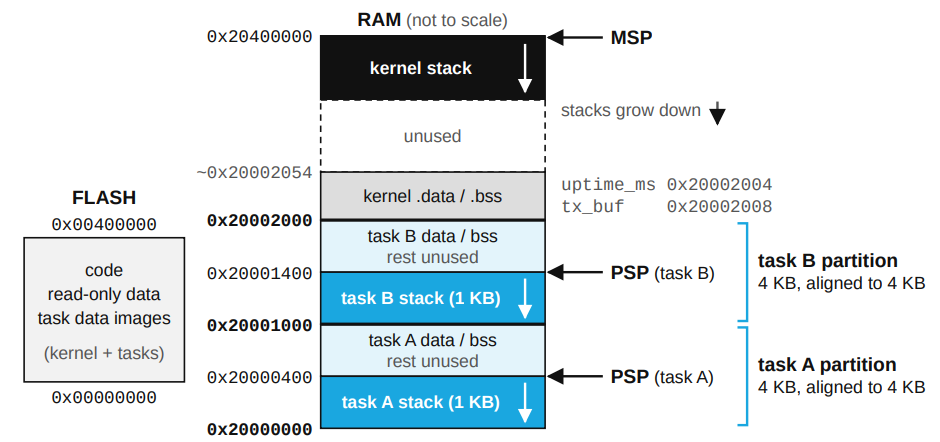
\includegraphics[width=0.7\textwidth]{contents/images/week-04/PSP_and_MSP.png}
\end{figure}

The stack must be \textbf{inside the partition}: it holds locals, return addresses and the exception frames. If it lived in kernel RAM, you could not restrict a task to its own 4 KB without taking its stack away. And since handler mode always uses MSP, the kernel's work (interrupts, system calls) never runs on a task's stack.

\subsection{Starting a Task: \texttt{task\_launch} and the Fake Frame}

\paragraph*{Why use a Fake Stack Frame?}

The kernel cannot simply launch a user task using a standard function call. Because the kernel operates in \textbf{Handler Mode} (using the Main Stack Pointer, MSP, with full privileges), a standard call would cause the task to inherit this exact state. This would destroy system isolation, as a bug in the user task could silently corrupt kernel memory or crash the entire system.

To safely execute, a user task must run in a strictly confined environment:
\begin{enumerate}
    \item In \textbf{Thread Mode} (normal execution state).
    \item \textbf{Unprivileged} (restricted access to system registers and memory).
    \item On its own \textbf{Process Stack Pointer (PSP)}.
\end{enumerate}

On the ARM Cortex-M architecture, there is no single instruction to simultaneously change the stack pointer, drop privileges, switch execution modes, and jump to a new address. The \emph{only} hardware mechanism capable of performing this critical ``triple jump'' safely and atomically is an \textbf{Exception Return}.

Since a newly created task has never actually been interrupted, the kernel must trick the hardware by \textbf{faking an interrupt context}:
\begin{itemize}
    \item \textbf{Faking the past:} The kernel manually crafts an 8-word (32-byte) frame on the task's stack. This contains the exact layout of data the hardware would expect to find if the task had been previously running and then interrupted (including the starting \texttt{pc} and the \texttt{xPSR} status register).
    \item \textbf{Triggering the mechanism:} The kernel points the PSP to this newly created frame and commands the CPU to return from the current interrupt using the magic code \texttt{0xFFFFFFFD}.
    \item \textbf{The hardware restores:} The CPU blindly accepts the fake frame. It pops the registers from the PSP, drops its privileges, switches to Thread Mode, and jumps to the task's starting address, successfully launching it in the exact restricted conditions required by the Operating System.
\end{itemize}

\begin{figure}[h]
    \centering
    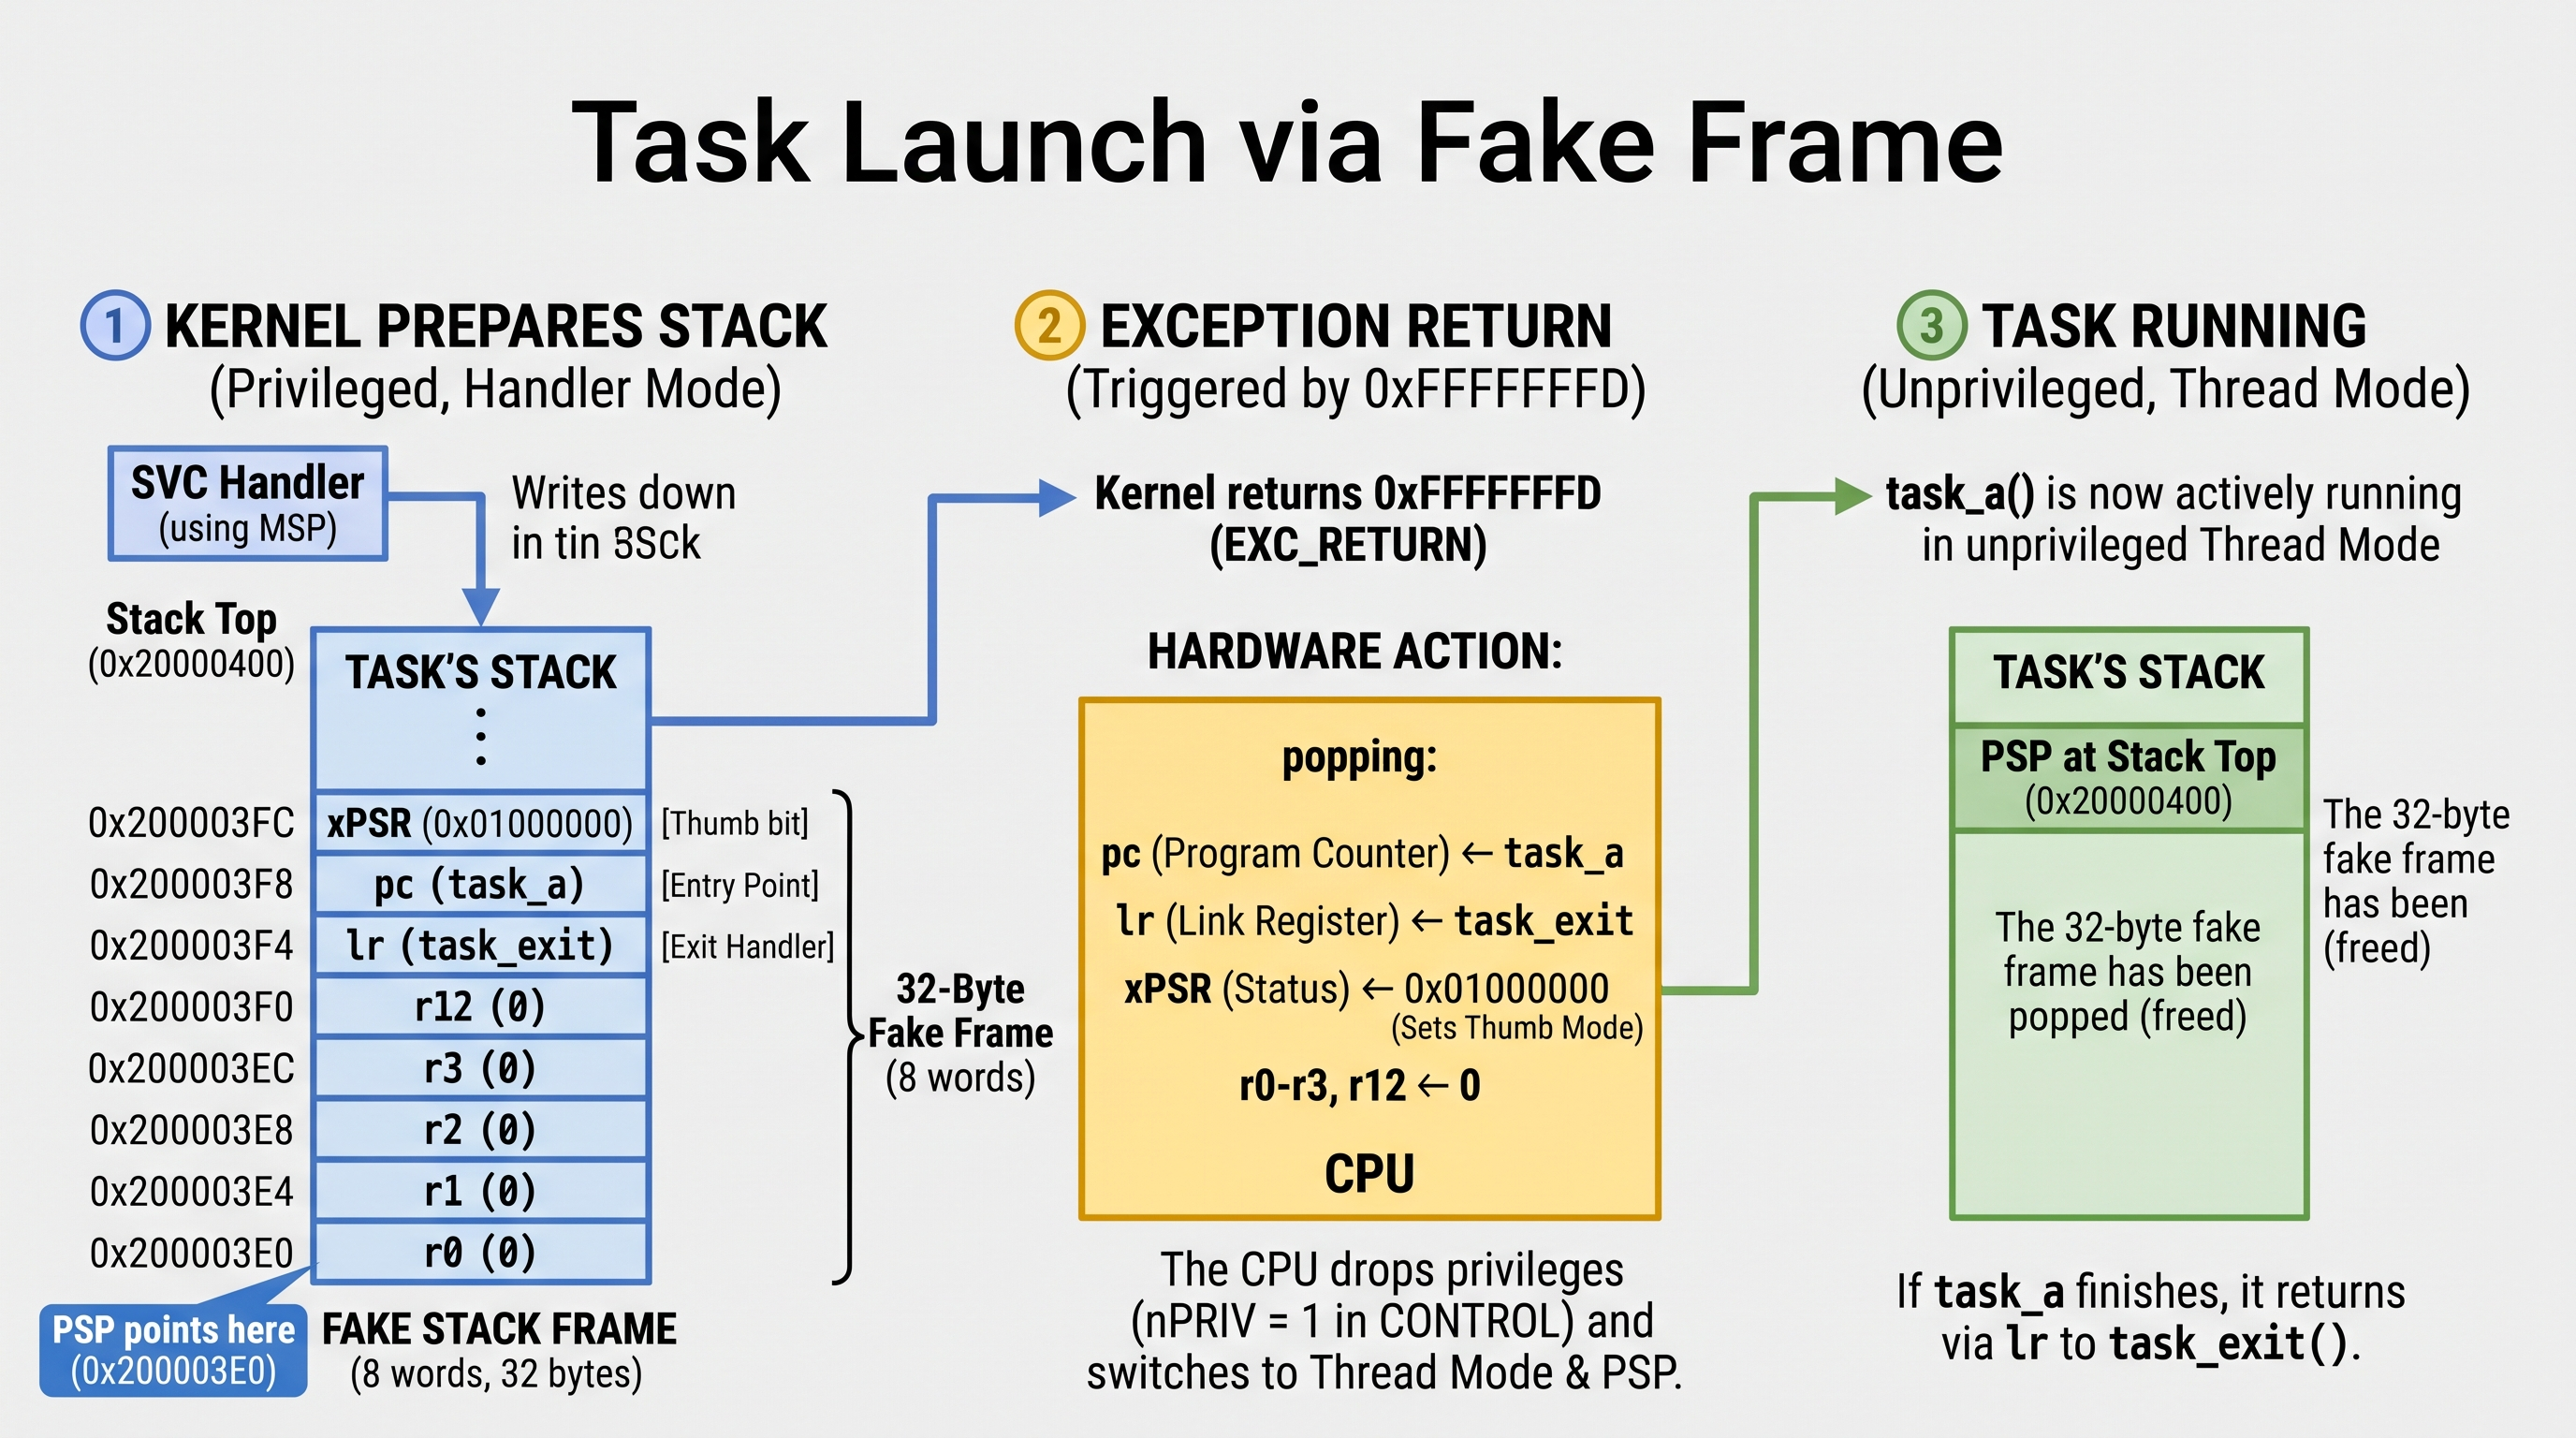
\includegraphics[width=0.7\textwidth]{contents/images/week-04/Fake_Frame.png}
\end{figure}

\paragraph*{The three steps of \texttt{task\_launch}}
The boot process starts from \texttt{main} with the \texttt{svc \#5} system call. The handler intercepts the call and launches \texttt{task\_launch()}, which performs three operations:

\begin{enumerate}
    \item \textbf{Bookkeeping:} records which task is starting, prepares the MPU to protect its partition, and initializes its RAM variables (\texttt{partition\_init()}).
    
    \item \textbf{Manual Frame Creation:} allocates 8 words (32 bytes) just below the task's stack top to set up the initial CPU context.

    \begin{center}
    \begin{tabular}{|l|l|p{8cm}|}
    \hline
    \textbf{Index} & \textbf{Register} & \textbf{Value and Purpose} \\
    \hline
    \texttt{frame[0..4]} & \texttt{r0--r3, r12} & \texttt{0} (unused at startup). \\
    \hline
    \texttt{frame[5]} & \texttt{lr} (Link) & \texttt{task\_exit}: if the task function returns, it will jump here to exit cleanly instead of crashing. \\
    \hline
    \texttt{frame[6]} & \texttt{pc} (Program) & The task's entry point address (e.g., \texttt{task\_a}). \\
    \hline
    \texttt{frame[7]} & \texttt{xPSR} & \texttt{0x01000000}: sets the \textbf{Thumb bit}. Mandatory on Cortex-M processors; without it, a crash (\texttt{UsageFault}) occurs. \\
    \hline
    \end{tabular}
    \end{center}

    \item \textbf{Context Switch:} through an Assembly block, it loads the frame address into the \texttt{PSP} register, sets the \texttt{nPRIV} bit in the \texttt{CONTROL} system register (to drop privileges), and forces the return of the value \texttt{0xFFFFFFFD} (\texttt{EXC\_RETURN\_THREAD\_PSP}).
\end{enumerate}

\paragraph*{The final result}
When the handler returns \texttt{0xFFFFFFFD}, the hardware "falls for" the fake exception: it pops the 32 bytes, restoring the registers as dictated by the frame. Execution thus jumps to the task's \texttt{pc} (Thread mode, unprivileged), while the \texttt{PSP}, freed from the frame, sits exactly at the top of the stack, ready for standard program execution.

\subsection{SVC\_Handler and SVC\_dispatch}
In the basic version of our OS, system calls (\texttt{svc}) always returned to the exact same place they came from. Now, things are more complex because an \texttt{svc} can be triggered from two different environments:
\begin{enumerate}
    \item From \textbf{main()}: just once, to start the OS. It uses the \textbf{MSP} (Main Stack Pointer).
    \item From \textbf{tasks}: for standard system calls. They use the \textbf{PSP} (Process Stack Pointer).
\end{enumerate}

\begin{figure}[h]
    \centering
    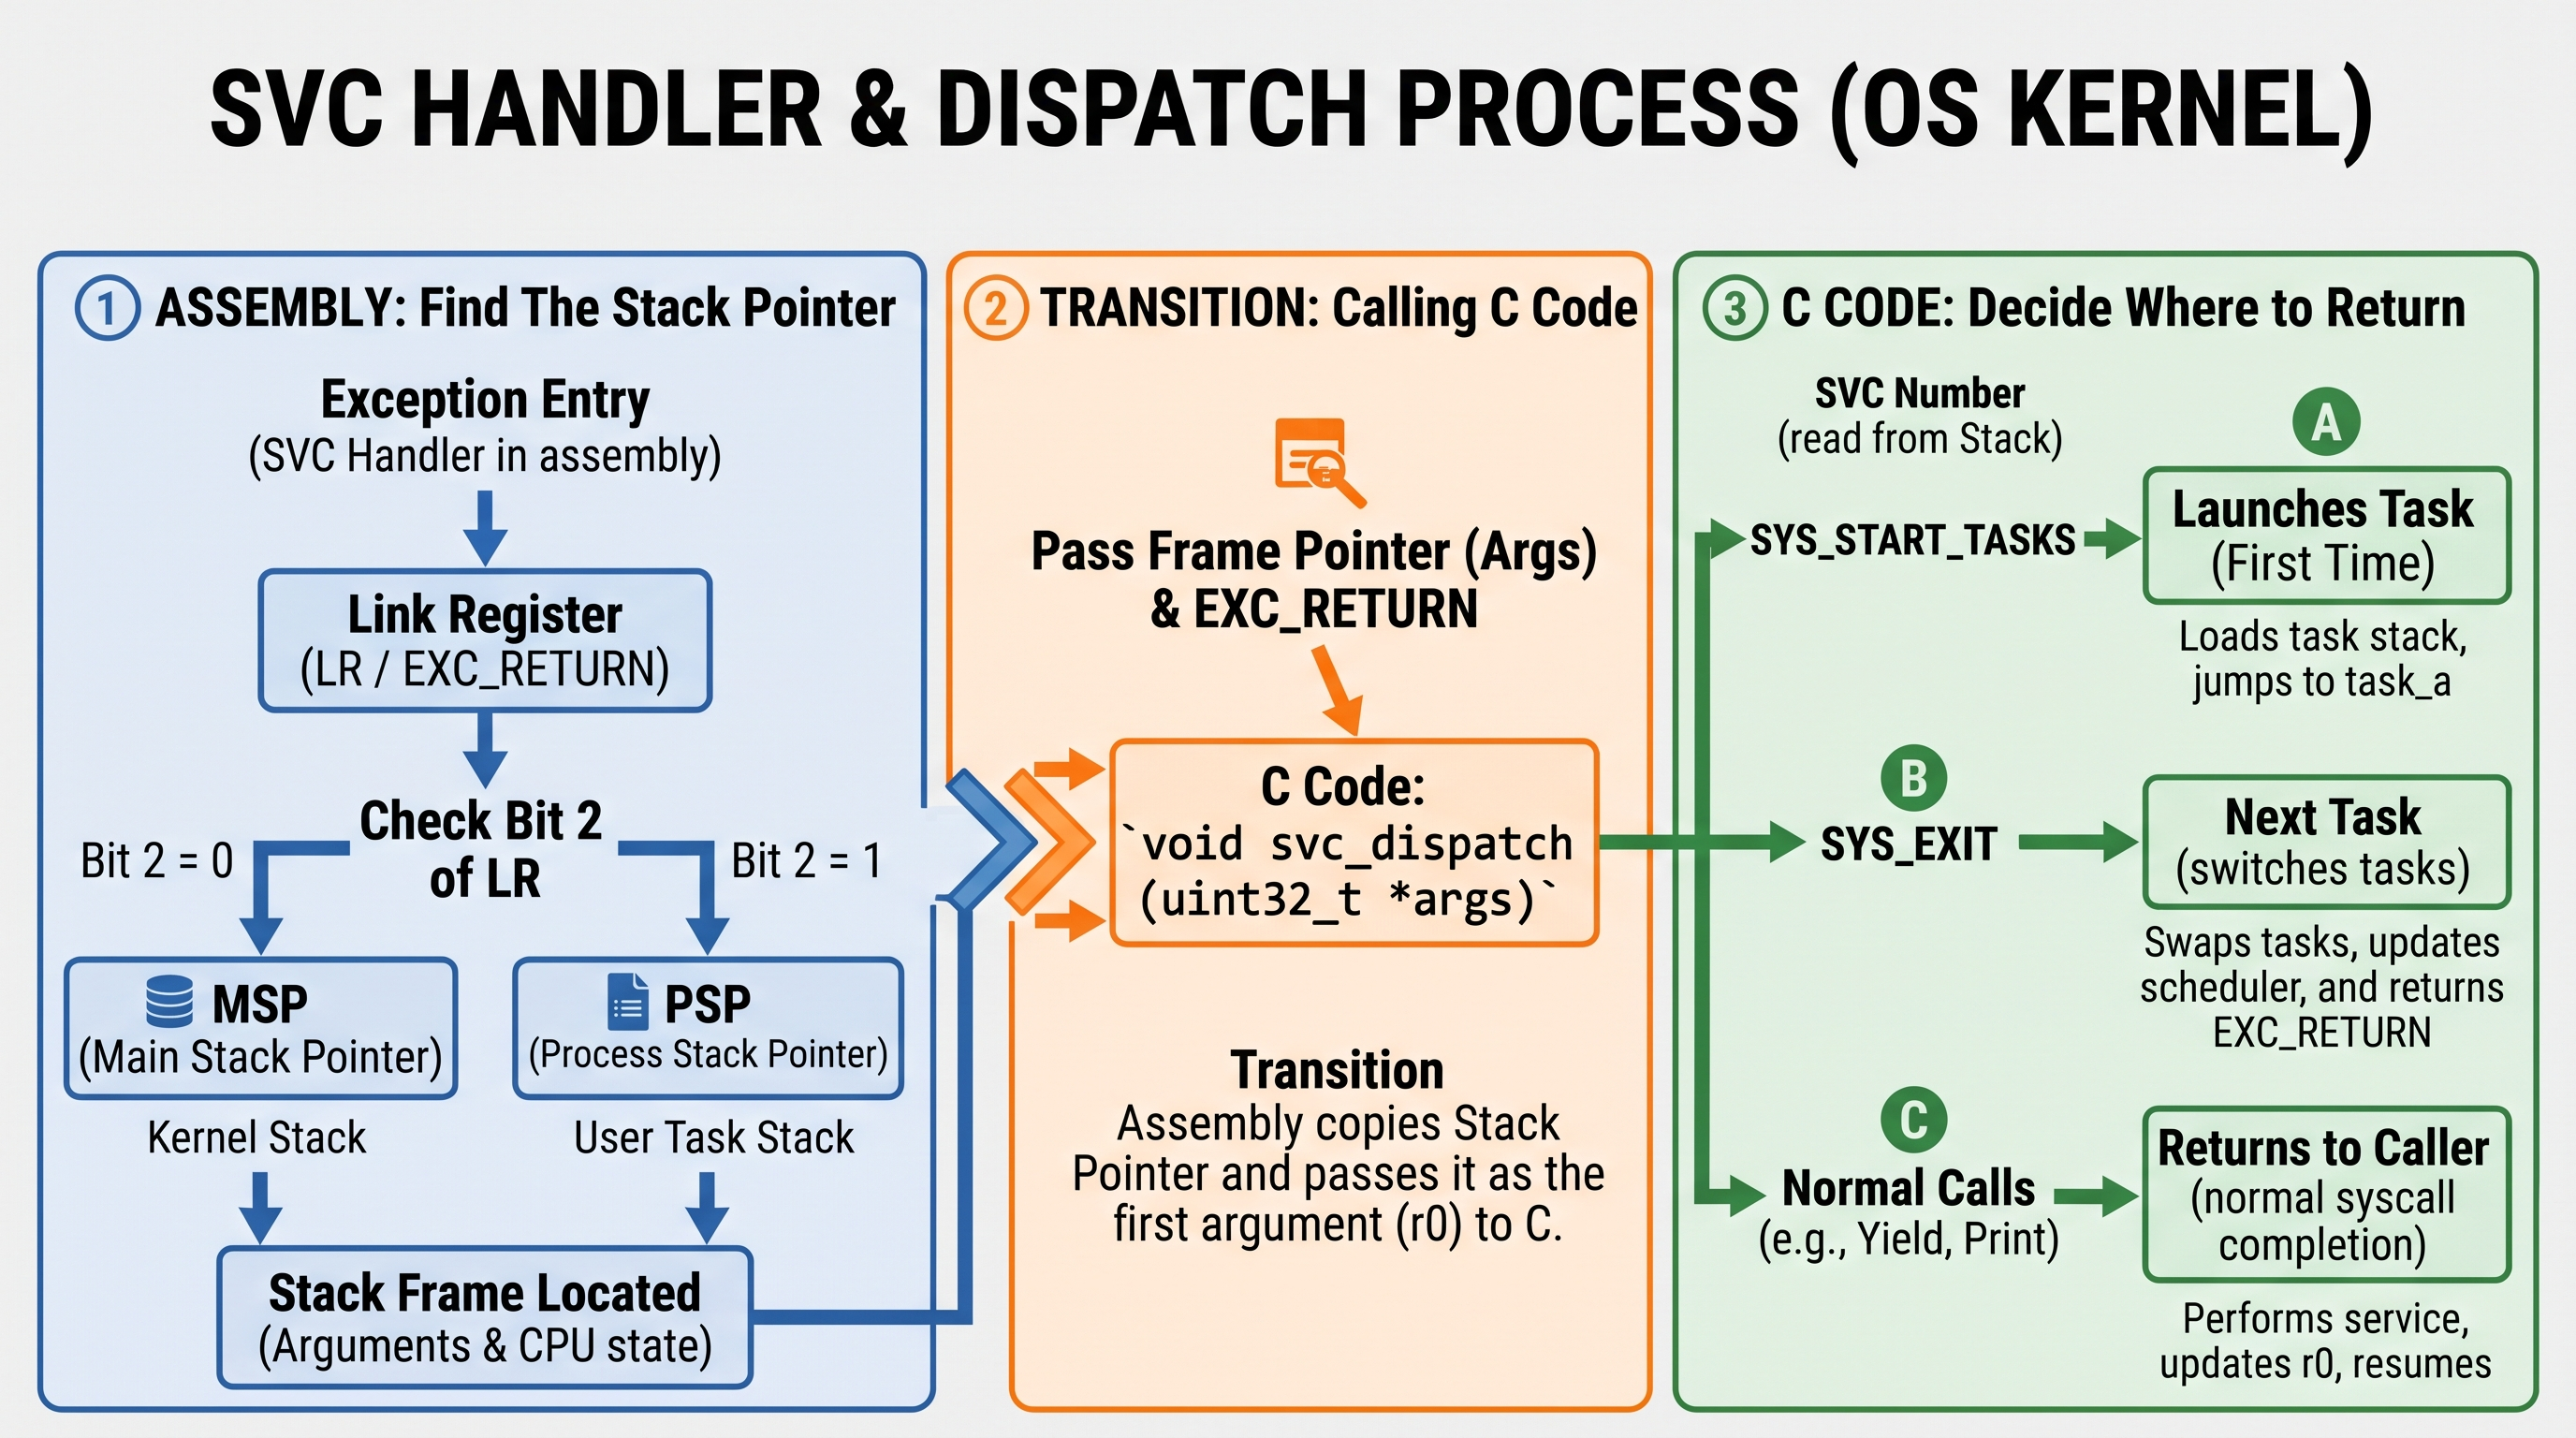
\includegraphics[width=0.7\textwidth]{contents/images/week-04/SVC_Handler_and_Dispatcher.png}
\end{figure}

\paragraph*{1. Finding the right Stack (Assembly)}
When the handler starts, it needs to find the saved CPU state (the frame). To know which stack was active, the hardware leaves a clue in the \textbf{Link Register (lr)} called the \texttt{EXC\_RETURN} code. 
By checking \textbf{bit 2} of this code, the handler knows where to look:
\begin{itemize}
    \item \texttt{0xFFFFFFF9} (bit 2 is \textbf{0}): The frame is on the \textbf{MSP}.
    \item \texttt{0xFFFFFFFD} (bit 2 is \textbf{1}): The frame is on the \textbf{PSP}.
\end{itemize}

Here is how the assembly checks this and calls the C dispatcher:
\begin{lstlisting}
    tst lr, #4        /* Check bit 2 of LR (LR AND 4) */
    ite eq            /* If-Then-Else based on the result */
    mrseq r0, msp     /* IF bit 2 == 0: r0 = MSP */
    mrsne r0, psp     /* ELSE bit 2 == 1: r0 = PSP */
    
    mov r1, lr        /* r1 = exc_return (save LR before calling C) */
    bl svc_dispatch   /* Call C: r0 = svc_dispatch(r0=frame, r1=exc_return) */
    bx r0             /* Return from exception using the code C gave us in r0 */
\end{lstlisting}

\paragraph*{2. Directing the Flow (C code)}
Previously, the assembly handler ended with a simple branch (\texttt{b}) to go back. However, calls like \texttt{SYS\_START\_TASKS} and \texttt{SYS\_EXIT} must change the flow entirely (e.g., leaving \texttt{main} to enter a task). 

To achieve this, \texttt{svc\_dispatch} is now responsible for deciding \textbf{where to return}. It takes the frame and the original \texttt{EXC\_RETURN} code as arguments, and \textbf{returns a new EXC\_RETURN code} back to the assembly:

\begin{lstlisting}[language=C]
uint32_t svc_dispatch( uint32_t *frame, uint32_t exc_return )
\end{lstlisting}

Inside the C function, it handles three specific scenarios:
\begin{itemize}
    \item \textbf{\texttt{SYS\_START\_TASKS}:} Instead of returning to \texttt{main}, it returns \texttt{task\_start\_first()}, returning the code needed to launch Task A.
    \item \textbf{\texttt{SYS\_EXIT}:} The task is done. It returns \texttt{task\_exit\_current()}, giving the code to launch the next task or go back to \texttt{main}.
    \item \textbf{Normal calls (Read/Write/etc.):} The kernel simply writes the function's result into \texttt{frame[0]} (which becomes \texttt{r0} for the task) and returns the \textbf{original} \texttt{exc\_return}. Execution resumes exactly where it left off.
\end{itemize}

By doing this, the kernel respects a golden rule: \textbf{it never waits inside a handler}. Every system call ends immediately, smoothly guiding the CPU into whatever should run next.

\subsection{How a Task Ends: \texttt{task\_exit} and \texttt{sys\_exit}}

The user side is in \texttt{lib/syscalls.s}. \texttt{sys\_exit} is a stub with the new number \texttt{SYS\_EXIT} (4); since it never returns, it ends with a branch to itself instead of \texttt{bx lr}. \texttt{task\_exit} is the address that \texttt{task\_launch} puts in \texttt{frame[5]}, the task's \texttt{lr}:

\begin{lstlisting}
sys_exit:                       task_exit:
    svc #4                          bl sys_exit    /* does not come back */
    b sys_exit                      b task_exit    /* never reached */
\end{lstlisting}

\begin{figure}[h]
    \centering
    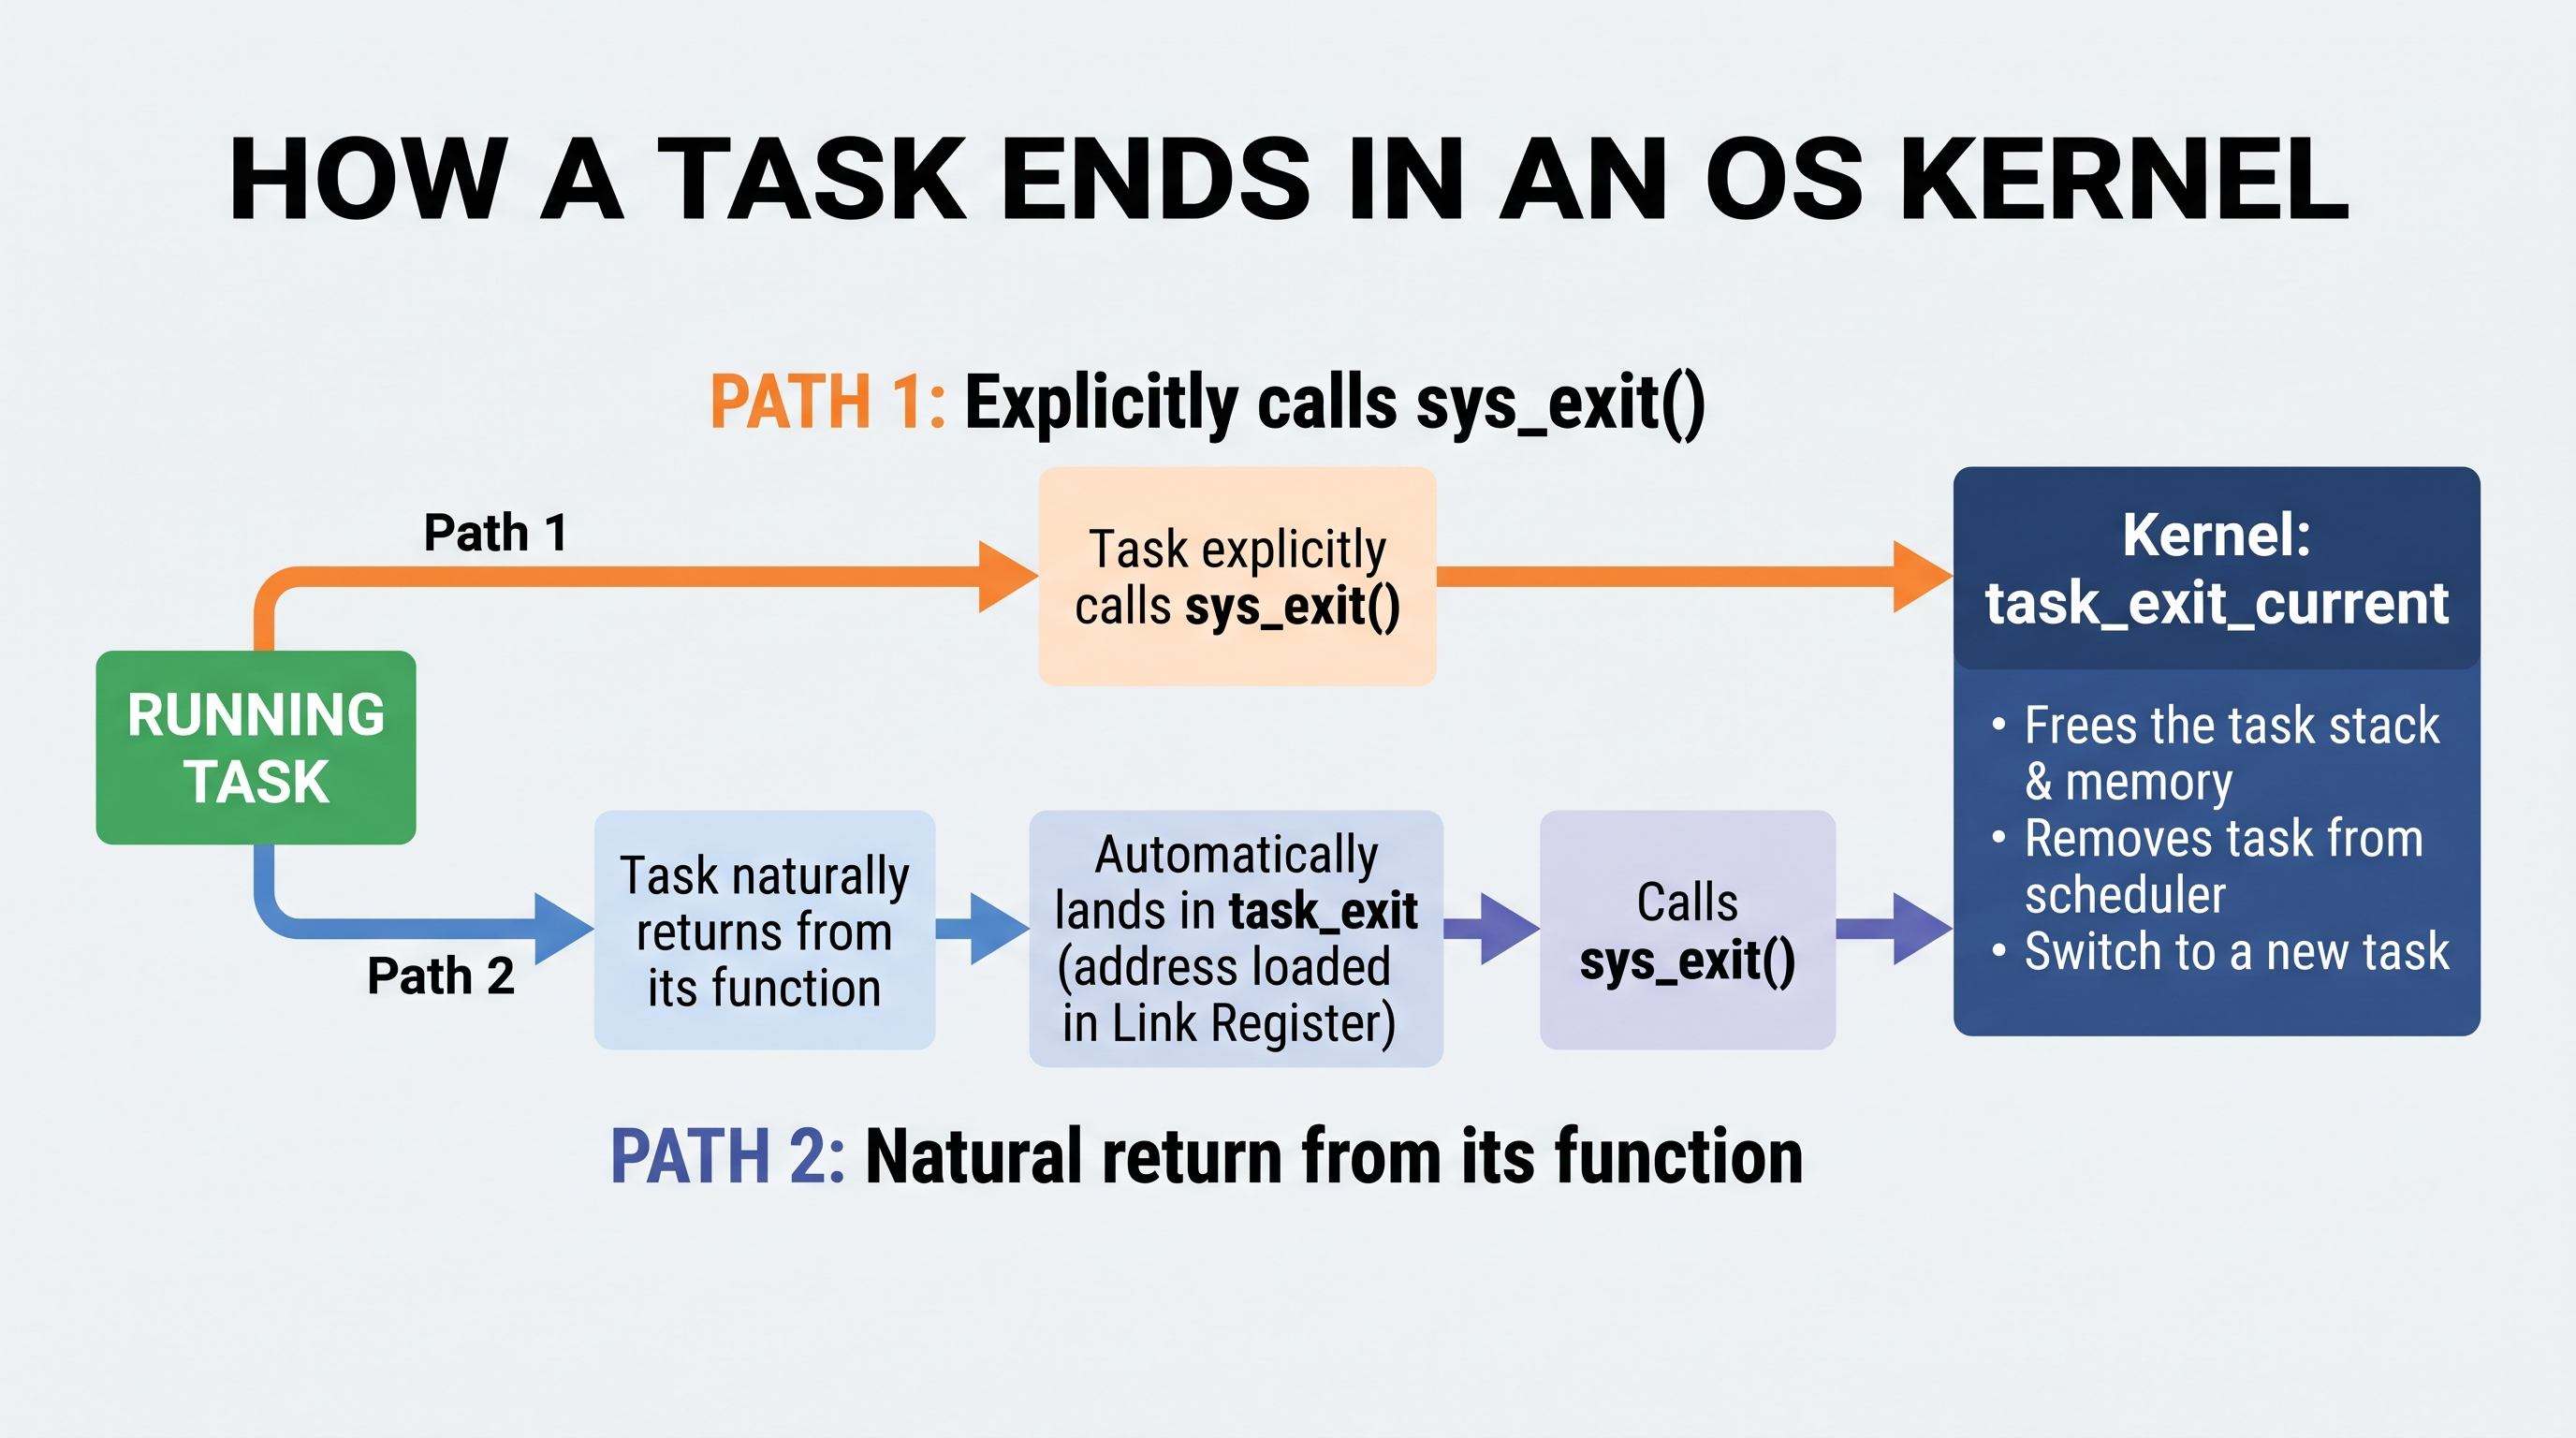
\includegraphics[width=0.7\textwidth]{contents/images/week-04/Exit_Task.png}
\end{figure}

A task can therefore end by calling \texttt{sys\_exit()} itself, or simply by returning from its function, landing in \texttt{task\_exit}; Task A uses the second way. The kernel side, \texttt{task\_exit\_current}, is read in Unit 3.

\subsection{The Two Stacks in gdb}

With \texttt{make debug}, then \texttt{arm-none-eabi-gdb build/scratch-os.axf}, \texttt{target remote :1234}, \texttt{break *task\_a}, \texttt{break *task\_b}, \texttt{continue}, and \texttt{p/x \$control}, \texttt{p/x \$psp}, \texttt{p/x \$msp}, \texttt{x/8wx \$psp-32} at each stop (the \texttt{*} stops at the very first instruction, before any push), you measure:

\begin{itemize}
    \item \textbf{CONTROL = 3} in both tasks (unprivileged, on PSP).
    \item \textbf{PSP} is \texttt{0x20000400} in A and \texttt{0x20001400} in B: the top of the bottom 1 KB of each partition, so inside its own partition.
    \item The popped \textbf{frame} still shows \texttt{lr = 0xb37} (\texttt{task\_exit} plus 1, the Thumb bit), pc = \texttt{task\_a} or \texttt{task\_b}, and \texttt{xPSR = 0x01000000}.
    \item \textbf{MSP} is \texttt{0x203fffd8} in both: it holds \texttt{main}'s waiting frame, and tasks never touch MSP.
\end{itemize}

\subsection{The Rogue Task, Partitioned}

Running \texttt{make run DEMO=rogue} again (\texttt{make} rebuilds \texttt{build/demo-rogue/}), Task B still stores \texttt{0x12345678} into \texttt{uptime\_ms}, now at \texttt{0x20002004}, outside B's partition, and the clock is corrupted \textbf{exactly as in Unit 1}. The linker only decided \textbf{where} things are: a store to \texttt{0x20002004} is an ordinary store, and nothing at run time compares it with B's partition \texttt{0x20001000}--\texttt{0x20002000}. Partitions \textbf{arrange} memory but do not \textbf{enforce} anything. What has changed is its shape: each task's memory is now one aligned 4 KB block, so one hardware rule per task is enough to describe what it may touch. That rule is Unit 3.

\subsection{End of Unit 2}

\begin{itemize}
    \item A \textbf{partition} is a fixed slice of RAM for one task, 4 KB and aligned to 4 KB, with the stack at the bottom and the variables above it; code and read-only data stay shared in FLASH.
    \item The linker builds partitions with \texttt{ALIGN(\dots, 4096)}, \texttt{(NOLOAD)} for stack and pad, \texttt{> RAM AT > FLASH} for the variables and \texttt{*task\_a.o(\dots)} to pick one file. The \textbf{first match wins}, so partition rules come before the kernel's, and \texttt{ASSERT} checks the size.
    \item \texttt{partition\_init} copies each task's variables, zeros included, from FLASH before the first run.
    \item Tasks run unprivileged on \textbf{PSP} with \textbf{CONTROL = 3}; the kernel and \texttt{main} use \textbf{MSP}.
    \item \texttt{task\_launch} writes an 8-word frame and returns \texttt{0xFFFFFFFD}, the only way into a task. \texttt{SVC\_Handler} finds the frame with \texttt{tst lr, \#4} and \texttt{svc\_dispatch} returns the EXC\_RETURN to use.
    \item \texttt{DEMO=rogue} still corrupts the kernel: the linker arranges memory but does not enforce anything.
\end{itemize}

\section{Unit 3: The MPU}

\subsection{The Cortex-M3 MPU: Regions}

Unit 1 introduced the MPU as a short list of regions checked on every access. On this CPU:

\begin{itemize}
    \item There are \textbf{8 regions}, numbered 0 to 7 (\texttt{MPU\_TYPE} bits 15:8 hold the count; on this board it reads \texttt{0x800}, that is 8).
    \item Each region has a \textbf{base address}, a \textbf{size} and \textbf{permissions}, and counts only when its ENABLE bit is set.
    \item The \textbf{size} is a power of two of at least 32 bytes, up to 4 GB.
    \item The \textbf{base must be a multiple of the size} (aligned to its size): a 4 KB region can start at \texttt{0x20000000} or \texttt{0x20001000}, not at \texttt{0x20000400}. This is why Unit 2 made each partition 4 KB and aligned to 4 KB: one region covers one partition exactly.
    \item When an \textbf{unprivileged} access falls in no enabled region, or its region refuses it, the access is \textbf{stopped} and the CPU raises a MemManage fault.
    \item For \textbf{privileged} code, the bit \textbf{PRIVDEFENA} chooses between the same rule and the board's default memory map wherever no region matches.
\end{itemize}

The MPU is a \textbf{core peripheral} at \texttt{0xE000ED90} and above, writable only by privileged code, so a task cannot switch it off.

\subsection{Permissions: AP, XN and PRIVDEFENA}

\textbf{AP} (access permissions) is a 3-bit field with one right for privileged and one for unprivileged code:

\begin{center}
\begin{tabular}{|l|l|l|p{5cm}|}
\hline
\textbf{AP} & \textbf{Privileged} & \textbf{Unprivileged} & \textbf{Used here for} \\
\hline
\texttt{000} & no access & no access & \\
\hline
\texttt{001} & read/write & no access & \\
\hline
\texttt{010} & read/write & read-only & \\
\hline
\texttt{011} & read/write & read/write & the running task's partition (\texttt{MPU\_AP\_FULL\_RW}) \\
\hline
\texttt{110} & read-only & read-only & FLASH (\texttt{MPU\_AP\_RO}) \\
\hline
\end{tabular}
\end{center}

\textbf{XN} (execute never) forbids instruction \textbf{fetches} from the region (reads and writes follow AP). A partition holds data and stack, never code, so it gets XN: a task cannot run code it has written into RAM, which closes a classic attack.

\textbf{PRIVDEFENA} is bit 2 of \texttt{MPU\_CTRL}. When 1, a \textbf{privileged} access that hits no region uses the default memory map, so the kernel keeps access to all RAM and peripherals without a region for each, and only the tasks are restricted. When 0, even the kernel may touch only what the regions allow. This week uses PRIVDEFENA = 1: the kernel is trusted and the MPU's purpose is to contain the tasks.

\subsection{The MPU Registers}

\begin{center}
\begin{tabular}{|l|l|p{7cm}|}
\hline
\textbf{Register} & \textbf{Address} & \textbf{Fields used this week} \\
\hline
\texttt{MPU\_TYPE} & \texttt{0xE000ED90} & bits 15:8: number of regions (read-only) \\
\hline
\texttt{MPU\_CTRL} & \texttt{0xE000ED94} & bit 0 ENABLE (the MPU checks accesses); bit 2 PRIVDEFENA \\
\hline
\texttt{MPU\_RNR} & \texttt{0xE000ED98} & region number: which region \texttt{RBAR}/\texttt{RASR} refer to \\
\hline
\texttt{MPU\_RBAR} & \texttt{0xE000ED9C} & bits 31:5 base; bit 4 VALID; bits 3:0 REGION \\
\hline
\texttt{MPU\_RASR} & \texttt{0xE000EDA0} & bit 28 XN; bits 26:24 AP; bits 18:16 S, C, B; bits 5:1 SIZE; bit 0 ENABLE \\
\hline
\end{tabular}
\end{center}

There is one pair \texttt{RBAR}/\texttt{RASR} for all eight regions, and \texttt{RNR} selects the current one. As a shortcut, writing \texttt{RBAR} with \textbf{VALID} (bit 4) set also sets the region number from its REGION field, so a single write replaces \texttt{RNR} then \texttt{RBAR}; this week's code uses it.

The \textbf{SIZE} field (5 bits) holds $\log_2(\text{size}) - 1$, so a region has $2^{\text{SIZE}+1}$ bytes; the $- 1$ lets 5 bits reach 4 GB. \textbf{S, C, B} (shareable, cacheable, bufferable) describe the memory type for caches and multi-core systems; this CPU has no cache, so they change nothing here (the code sets C for FLASH, S and C for RAM). TEX and SRD stay at 0.

\subsection{This Week's Two Regions}

\begin{itemize}
    \item \textbf{Region 0} covers FLASH: base \texttt{0x00000000}, size 4 MB, read-only and executable, the same for every task (code and string constants).
    \item \textbf{Region 1} covers the partition of the task running \textbf{now}, read/write and XN. The kernel moves it every time it starts a task.
    \item \textbf{Everything else} has \textbf{no region} for unprivileged code: the other task's partition, kernel data and stack, every peripheral. Any access by a task there causes a fault.
\end{itemize}

The ``MPU state'' of a task is therefore just one value: the base address of Region 1.

\subsection{Computing SIZE, RBAR and RASR}

\textbf{SIZE} $= \log_2(\text{size}) - 1$; since it sits in bits 5:1 it is multiplied by 2 before ENABLE (bit 0) is added:

\begin{itemize}
    \item Partition: $4096 = 2^{12}$, SIZE $= 11$ (\texttt{0b01011}); $11 \times 2 = $ \texttt{0x16}, with ENABLE \texttt{0x17}.
    \item FLASH: $4\text{ MB} = 2^{22}$, SIZE $= 21$ (\texttt{0b10101}); $21 \times 2 = $ \texttt{0x2A}, with ENABLE \texttt{0x2B}.
\end{itemize}

\textbf{RBAR} $=$ base $|$ VALID (\texttt{0x10}) $|$ region number: Region 0 gives \texttt{0x00000010}; Region 1 gives \texttt{0x20000011} for Task A and \texttt{0x20001011} for Task B. The base fills bits 31:5 and a base aligned to a size of at least 32 always ends in five 0 bits, leaving room for VALID and REGION.

\textbf{RASR} of Region 1 for Task B is \texttt{0x13060017}:

\begin{center}
\begin{tabular}{|l|l|l|p{5.2cm}|}
\hline
\textbf{Bits} & \textbf{Field} & \textbf{Value} & \textbf{Meaning} \\
\hline
28 & XN & 1 & no instruction fetch (\texttt{0x10000000}) \\
\hline
26:24 & AP & \texttt{011} & read/write for both (\texttt{0x03000000}) \\
\hline
18, 17 & S, C & 1, 1 & shareable, cacheable (\texttt{0x00060000}) \\
\hline
5:1 & SIZE & 11 & $2^{12}$ = 4 KB (\texttt{0x16}) \\
\hline
0 & ENABLE & 1 & region on (\texttt{0x01}) \\
\hline
\end{tabular}
\end{center}

The sum is \texttt{0x10000000 + 0x03000000 + 0x00060000 + 0x16 + 0x01 = 0x13060017}. Region 0 is built the same way, from AP \texttt{110} (\texttt{0x06000000}), C (\texttt{0x00020000}) and \texttt{0x2B}, without XN: \texttt{0x0602002B}.

\textbf{Three exercises:}
\begin{itemize}
    \item \textit{A 32 KB region: SIZE and low byte of \texttt{RASR}?} $32\text{ KB} = 2^{15}$, SIZE $= 14$, $14 \times 2 = $ \texttt{0x1C}, with ENABLE \textbf{\texttt{0x1D}}.
    \item \textit{Could it start at \texttt{0x20001000}?} \textbf{No}: the base must be a multiple of 32 KB (\texttt{0x8000}); \texttt{0x20000000} and \texttt{0x20008000} are valid.
    \item \textit{A task needs 5 KB: which region size?} \textbf{8 KB}, the next power of two (3 KB unused), the same price as for Unit 2's partitions.
\end{itemize}

\subsection{Helpers and Prepared Calls}

\begin{itemize}
    \item \textbf{\texttt{MPU\_RASR\_SIZE( n )}} (\texttt{include/cmsdk.h}) takes $n = \log_2(\text{size})$ and computes \texttt{((n) - 1) << 1}: write \texttt{MPU\_RASR\_SIZE( 22 )} for 4 MB and \texttt{( 12 )} for 4 KB.
    \item \textbf{\texttt{\_\_builtin\_ctz( x )}} (GCC) counts the trailing 0 bits of \texttt{x}; for a power of two this is its $\log_2$ (\texttt{\_\_builtin\_ctz( 4096 )} is 12).
    \item \textbf{\texttt{dsb}} waits until every earlier write has really finished and \textbf{\texttt{isb}} then makes the following instructions see the new settings; after writing MPU registers you use both, so no later access is checked against the old regions.
\end{itemize}

\texttt{cmsdk.h} also gives the registers as a \texttt{struct} (\texttt{MPU->CTRL}, \texttt{MPU->RBAR}, \texttt{MPU->RASR}, \dots) and one macro per field (\texttt{MPU\_RBAR\_VALID}, \texttt{MPU\_RASR\_XN}, \texttt{MPU\_RASR\_AP( v )} with \texttt{MPU\_AP\_RO} and \texttt{MPU\_AP\_FULL\_RW}, \texttt{MPU\_RASR\_S}, \texttt{\_C}, \texttt{\_ENABLE}, \texttt{MPU\_CTRL\_ENABLE}, \texttt{MPU\_CTRL\_PRIVDEFENA}). The calls are prepared: \texttt{main} calls \texttt{mpu\_init()} once before its \texttt{svc \#5}, and \texttt{task\_launch} calls \texttt{mpu\_set\_task\_region( part\_start, part\_end - part\_start )} before entering each task. In the base both bodies are empty, so the MPU is off.

\subsection{Writing \texttt{mpu\_init} and \texttt{mpu\_set\_task\_region}}

In \texttt{kernel/mpu.c} replace both functions, from \texttt{void mpu\_init( void )} to the end of the file. \texttt{mpu\_init} programs Region 0 and switches the MPU on:

\begin{lstlisting}[language=C]
void mpu_init( void )
{
    /* Region 0 = FLASH: base 0, 4 MB = 2^22 B, read-only, code may run. */
    MPU->RBAR = 0x00000000 | MPU_RBAR_VALID | 0;         /* = 0x00000010 */
    MPU->RASR = MPU_RASR_AP( MPU_AP_RO ) | MPU_RASR_C
              | MPU_RASR_SIZE( 22 ) | MPU_RASR_ENABLE;   /* = 0x0602002B */

    /* MPU on. PRIVDEFENA: the kernel keeps the default memory map. */
    MPU->CTRL = MPU_CTRL_ENABLE | MPU_CTRL_PRIVDEFENA;    /* = 5 */
    __asm volatile ( "dsb" ::: "memory" );   /* finish the writes ... */
    __asm volatile ( "isb" ::: "memory" );   /* ... before the next instruction */
}
\end{lstlisting}

After reset the MPU is disabled: until \texttt{ENABLE} is set in \texttt{MPU->CTRL}, no protection is enforced however the regions are programmed. Region 1 is not set yet, but this is not a problem: \texttt{main} and the kernel are privileged and keep the default map through \texttt{PRIVDEFENA}, and no unprivileged code runs before \texttt{task\_launch} sets Region 1. The second function is called by \texttt{task\_launch} every time a task starts, and moves Region 1 onto that task's partition:

\begin{lstlisting}[language=C]
void mpu_set_task_region( uint32_t base, uint32_t size )
{
    /* log2 of a power of two = its trailing zero bits: 4096 -> 12. */
    uint32_t log2_size = __builtin_ctz( size );

    /* Region 1 = the partition: read-write, never executable (XN). */
    MPU->RBAR = base | MPU_RBAR_VALID | 1;                /* B: 0x20001011 */
    MPU->RASR = MPU_RASR_XN | MPU_RASR_AP( MPU_AP_FULL_RW )
              | MPU_RASR_S | MPU_RASR_C
              | MPU_RASR_SIZE( log2_size ) | MPU_RASR_ENABLE; /* 0x13060017 */
    __asm volatile ( "dsb" ::: "memory" );
    __asm volatile ( "isb" ::: "memory" );
}
\end{lstlisting}

The function computes SIZE from the size it receives, which must be a power of two with \texttt{base} a multiple of it (the linker script guarantees both). The lines \texttt{(void) base;} and \texttt{(void) size;} of the base disappear: they only silenced ``unused parameter'' warnings while the body was empty. \texttt{make} now builds with no errors and no warnings.

\subsection{Catching Violations: The MemManage Fault}

When the MPU refuses an access, the access does \textbf{not} happen (a store writes nothing, a load reads nothing) and the CPU raises \textbf{MemManage}, exception 4, enabled at boot by \texttt{MEMFAULTENA} in \texttt{SHCSR} (Week 2). \texttt{MemManage\_Handler} in \texttt{kernel/faults.c} runs privileged on the MSP. The low byte of \textbf{CFSR} (\texttt{0xE000ED28}) tells why:

\begin{center}
\begin{tabular}{|c|l|p{7.8cm}|}
\hline
\textbf{Bit} & \textbf{Name} & \textbf{Set when} \\
\hline
0 & \texttt{IACCVIOL}  & an \textbf{instruction fetch} was refused (for example from an XN region) \\
\hline
1 & \texttt{DACCVIOL}  & a \textbf{data} load or store was refused \\
\hline
3 & \texttt{MUNSTKERR} & popping a frame on \textbf{exception return} was refused \\
\hline
4 & \texttt{MSTKERR}   & pushing the 8-word frame on \textbf{exception entry} (stacking) was refused \\
\hline
7 & \texttt{MMARVALID} & \textbf{MMFAR} holds the refused address \\
\hline
\end{tabular}
\end{center}

\textbf{MMFAR} (\texttt{0xE000ED34}, \texttt{SCB->MMFAR}) holds the refused data address. Read it only if \texttt{MMARVALID} is 1: for a fetch or stacking fault the CPU does not write it, and it may hold a stale value. Several bits can be set at once.

\textbf{Reporting the address.} In \texttt{MemManage\_Handler}, replace the line \texttt{kprintf( "MemManage: CFSR=0x\%x\textbackslash n", SCB->CFSR );} and the comment \texttt{/* >>> UNIT 3: report MMFAR and the cause bits here. <<< */} with the code below (the \texttt{halt();} that follows stays):

\begin{lstlisting}[language=C]
    uint32_t cfsr = SCB->CFSR;
    kprintf( "MemManage: CFSR=0x%x\n", cfsr );

    /* MMFAR holds a real address only when MMARVALID is set. */
    if ( cfsr & SCB_CFSR_MMARVALID )
        kprintf( "  address 0x%x\n", SCB->MMFAR );

    /* Name the cause. Several bits can be set at once. */
    if ( cfsr & SCB_CFSR_DACCVIOL )
        kprintf( "  cause: data access\n" );
    if ( cfsr & SCB_CFSR_IACCVIOL )
        kprintf( "  cause: instruction fetch\n" );
    if ( cfsr & SCB_CFSR_MSTKERR )
        kprintf( "  cause: stacking\n" );
\end{lstlisting}

\texttt{CFSR} is read once so that every test sees the same value, and the cause tests are separate \texttt{if}s rather than an \texttt{else if} chain because several bits can be set together. The masks \texttt{SCB\_CFSR\_...} are in \texttt{include/cmsdk.h}. \texttt{kprintf} works inside the handler because the handler is privileged.

\subsection{Running with the MPU On: Protection in Action}

Once the MPU is active, it strictly enforces the memory boundaries set by the linker. Here is how it affects different execution scenarios:

\paragraph*{1. The Normal Run (\texttt{make run})}
The system behaves exactly as in previous units, but now under hardware supervision. Tasks A and B run correctly because the MPU permits access to only two areas:
\begin{itemize}
    \item \textbf{Region 0 (FLASH):} Where the code and string constants reside.
    \item \textbf{Region 1 (Task Partition):} Where the task's variables, stack, and local buffers (like the \texttt{printf} buffer) live. 
\end{itemize}
When a task calls \texttt{sys\_write} or \texttt{sys\_uptime}, the context switches to the kernel (Handler Mode). The kernel is privileged and bypasses the MPU's user restrictions, freely accessing the UART and kernel data. As the OS switches from Task A to Task B, the MPU's Region 1 is simply updated on the fly to point to B's partition instead of A's.

\paragraph*{2. The Rogue Task (\texttt{DEMO=rogue})}
If Task B maliciously (or accidentally) attempts to overwrite a kernel variable like \texttt{uptime\_ms}, the MPU intervenes instantly. The store instruction \textbf{never executes}. Instead, the hardware halts the task and triggers a \textbf{MemManage Fault}:

\begin{lstlisting}
B: writing to the kernel's uptime counter
MemManage: CFSR=0x82
  address 0x20002004
  cause: data access
\end{lstlisting}

\begin{itemize}
    \item \textbf{\texttt{0x82} (DACCVIOL + MMARVALID):} Means a data access was denied, and the faulting address is securely recorded.
    \item \textbf{\texttt{0x20002004}:} The exact address of \texttt{uptime\_ms}.
\end{itemize}
The clock remains uncorrupted. The bug is caught exactly at the instruction that caused it, rather than causing a mysterious failure later.

\paragraph*{3. The Stack Overflow (\texttt{DEMO=overflow})}
If Task B enters deep recursion (e.g., requesting 4 KB of stack space while only 1 KB is available), its stack pointer pushes past its lower boundary.

\begin{lstlisting}
B: recursing
MemManage: CFSR=0x92
  address 0x20000fdc
  cause: data access
  cause: stacking
\end{lstlisting}

\begin{itemize}
    \item \textbf{The Address (\texttt{0x20000fdc}):} This address sits just \emph{below} Task B's partition, plunging into Task A's territory. Since Region 1 only covers Task B, the MPU blocks the write (\textbf{DACCVIOL}).
    \item \textbf{The Stacking Error (\textbf{MSTKERR}):} When the fault occurs, the CPU attempts to save its 8-word state frame onto the active stack (PSP). Because the PSP is already out of bounds, this save operation is also blocked. 
\end{itemize}

This perfectly demonstrates why Unit 2 placed the stack at the \textbf{bottom} of the partition: the moment the stack overflows, it leaves the allowed memory region, immediately triggering a fault. Without the MPU, this overflow would silently crush Task A's data, eventually causing an incomprehensible crash far from the original error.

\subsection{Why the Kernel Must Validate Pointers (\texttt{DEMO=badptr})}

The MPU \textbf{does not} stop \texttt{DEMO=badptr}. When a task executes a system call like \texttt{sys\_write}, the CPU switches to \textbf{privileged mode} inside the \texttt{SVC\_Handler}. Because the kernel has full access to the memory map, it can read or write anywhere. If a task passes a pointer to kernel-private memory, the kernel will blindly access it on the task's behalf, inadvertently leaking or corrupting data.

To prevent this, the kernel must manually verify that every pointer provided by a task points \textbf{entirely} to memory that the task itself is allowed to access. For \texttt{sys\_write}, the buffer \texttt{[buf, buf + len)} must fall strictly inside either:
\begin{itemize}
    \item The caller's \textbf{RAM partition}.
    \item The \textbf{FLASH memory} (\texttt{0x00000000}--\texttt{0x00400000}), where string constants reside.
\end{itemize}

\paragraph*{The Danger of Integer Overflow}
To validate the buffer, the kernel uses the helper \texttt{in\_range(p, len, start, end)}. A naive check like \texttt{p + len <= end} is a severe security flaw: if \texttt{p = 0x20001F00} and \texttt{len = 0xFFFFFF00}, the sum wraps around modulo $2^{32}$ to \texttt{0x20001E00}. This passes the naive check, allowing the task to trick the kernel into reading almost all of RAM.

The secure implementation prevents wrap-around by isolating \texttt{len}:
\begin{lstlisting}[language=C]
static int in_range( uint32_t p, uint32_t len, uint32_t start, uint32_t end )
{
    /* If p <= end is true, end - p cannot wrap */
    return p >= start && p <= end && len <= end - p;
}
\end{lstlisting}

\paragraph*{Implementing the Check}
In \texttt{sys\_write\_impl}, the kernel inspects the caller using \texttt{task\_current()} (which returns \texttt{0} if the trusted kernel itself made the call):
\begin{lstlisting}[language=C]
    /* Accept the buffer only inside the caller's partition or inside
     * FLASH (string constants). The kernel itself (no task) is trusted. */
    const struct task *t = task_current();
    if ( t != 0
         && !in_range( a0, len, t->part_start, t->part_end )
         && !in_range( a0, len, 0x00000000, 0x00400000 ) )
        return ( uint32_t ) -1;
\end{lstlisting}

\paragraph*{The Result}
Running \texttt{make run DEMO=badptr} now yields:
\begin{lstlisting}
B: sys_write returned -1
B: uptime 4000 ms (second 1)
\end{lstlisting}
Because \texttt{0x20002004} (the kernel's uptime variable) is neither in B's partition nor in FLASH, \texttt{sys\_write} immediately returns \texttt{-1} before \texttt{uart\_write} is even called. No kernel data is leaked. 

Task B continues running safely because a refused system call is treated as a standard error that the task can handle, not a hardware fault. 

\textbf{The Takeaway:} The \textbf{MPU} stops unauthorized actions a task attempts directly. \textbf{Kernel pointer checks} stop unauthorized actions a task asks the kernel to perform. Both layers of security are strictly necessary.

\subsection{How a Task Ends: \texttt{task\_exit\_current}}

When a task finishes and triggers \texttt{SYS\_EXIT} (via \texttt{svc \#4}), the dispatcher calls \texttt{task\_exit\_current()}. This function must decide the next step: launch the next available task, or, if no tasks remain, safely shut down the OS and return to \texttt{main()}.

\begin{lstlisting}[language=C]
uint32_t task_exit_current( void )
{
    kprintf( "task %s exited\n", tasks[current].name );
    
    /* If there is another task in the list, start it */
    if ( current + 1 < ( int ) NUM_TASKS )
        return task_launch( current + 1 ); 

    /* Otherwise, no tasks are left. Return to main() */
    current = -1; 
    
    /* asm block: CONTROL = CONTROL & ~1;  (Clear nPRIV to regain privileges) */
    return EXC_RETURN_THREAD_MSP;          /* 0xFFFFFFF9: Thread mode, MSP */
}
\end{lstlisting}

The execution flow handles two distinct scenarios:

\paragraph*{1. Switching to the Next Task (e.g., Task A $\rightarrow$ Task B)}
When Task A ends, it naturally returns to the \texttt{task\_exit} stub, which triggers \texttt{sys\_exit}. The dispatcher catches this and executes \texttt{task\_exit\_current()}.
\begin{itemize}
    \item The kernel calls \texttt{task\_launch(1)} to prepare Task B.
    \item \textbf{The MPU Shift:} Inside \texttt{task\_launch}, the kernel updates the MPU. Region 1 is instantly shifted to cover Task B's partition (\texttt{RBAR = 0x20001011}). Task A's partition is stripped of its protection region, making it completely invisible and inaccessible to Task B.
    \item The handler returns \texttt{0xFFFFFFFD}, loading Task B's fake frame and starting its execution on the PSP.
\end{itemize}

\paragraph*{2. The Final Task Exits (Returning to \texttt{main})}
If the last task in the system were to exit, the kernel must hand control back to \texttt{main()}, which has been paused since the OS booted.
\begin{itemize}
    \item The kernel sets \texttt{current = -1} to indicate the OS is idle.
    \item \textbf{Restoring Privileges:} It clears the \texttt{nPRIV} bit in the \texttt{CONTROL} register. This is absolutely essential: \texttt{main()} runs in Thread Mode, and if it remained unprivileged, it would instantly trigger a Hardware Fault trying to access the UART to print its final message.
    \item The handler returns \texttt{0xFFFFFFF9}, switching the CPU back to the Main Stack Pointer (\textbf{MSP}) exactly where \texttt{main()} left off.
\end{itemize}

\textit{Note:} In the current Unit, you never actually see \texttt{main()} print its final success message because Task B contains an infinite loop and never exits.

\subsection{End of Unit 3}

For the tasks it runs, the kernel now does all four jobs of the week:

\begin{itemize}
    \item \textbf{Placement:} each task has a fixed 4 KB partition built by the linker (stack at the bottom, variables above); code and constants are shared in FLASH.
    \item \textbf{Separate stacks:} tasks run unprivileged on the PSP inside their partition, the kernel on the MSP; \texttt{task\_launch} enters a task by an exception return and \texttt{task\_exit\_current} ends it and starts the next.
    \item \textbf{Protection by the hardware:} the MPU allows a task FLASH (read and execute) and its own partition (read/write, no execute) and nothing else; a refused access raises MemManage, whose report gives cause and exact address (\texttt{rogue}: \texttt{0x82}; \texttt{overflow}: \texttt{0x92}).
    \item \textbf{Protection by the kernel:} \texttt{sys\_write} refuses any buffer the calling task could not read by itself (\texttt{badptr} gets $-1$), with an overflow-safe \texttt{in\_range}.
\end{itemize}

A correct program prints exactly the same output as in Unit 1; what has changed is what a \textbf{wrong} one can do.

\section{Where to Find the Code}

The files changed this week, all in \texttt{week-04/solution/} (\texttt{base/} is the starting point; if these notes and the code disagree, the code is the reference):

\begin{itemize}
    \item \texttt{scripts/mps2\_m3.ld}: the two partitions and their \texttt{ASSERT}s; \texttt{include/cmsdk.h}: MPU registers, field macros, \texttt{MMFAR}, CFSR masks.
    \item \texttt{kernel/task.h}, \texttt{task.c}: \texttt{struct task}, \texttt{partition\_init}, \texttt{task\_current}, \texttt{task\_launch}, \texttt{task\_start\_first}, \texttt{task\_exit\_current}.
    \item \texttt{kernel/svc\_entry.s}: \texttt{SVC\_Handler}; \texttt{kernel/syscall.c}: \texttt{svc\_dispatch}, \texttt{in\_range}, the checked \texttt{sys\_write\_impl}.
    \item \texttt{kernel/mpu.c}: \texttt{mpu\_init}, \texttt{mpu\_set\_task\_region}; \texttt{kernel/faults.c}: \texttt{MemManage\_Handler}.
    \item \texttt{lib/syscalls.s}, \texttt{syscalls.h}: \texttt{sys\_exit}, \texttt{task\_exit}, service numbers 4 and 5; \texttt{src/main.c}, \texttt{task\_a.c}, \texttt{task\_b.c}; \texttt{Makefile}: the \texttt{DEMO} switch.
\end{itemize}


\section{A prova di coglione}

\subsection{Unità 1}
\paragraph*{I compiti del Sistema Operativo}
La memoria è una risorsa condivisa. Un sistema operativo completo deve gestire quattro aspetti fondamentali:
\begin{itemize}
    \item \textbf{Collocazione (Placement):} assegnare indirizzi distinti a codice, dati e stack di ogni programma per evitare sovrapposizioni e corruzione dei dati.
    \item \textbf{Condivisione (Sharing):} permettere l'uso comune e sicuro di risorse (es. librerie, buffer hardware, aree di scambio dati tra processi).
    \item \textbf{Protezione (Protection):} impedire l'accesso accidentale o intenzionale alla memoria di altri task.
    \item \textbf{Espansione (Memoria Virtuale):} simulare una quantità di memoria superiore alla RAM fisica, appoggiandosi a memorie di massa.
\end{itemize}
Il codice di partenza del corso implementa esclusivamente una collocazione di base, e in modo parziale.

\paragraph*{Limiti del codice di partenza}
Ispezionando i binari compilati, si nota che il linker alloca le variabili del kernel e dei task utente una dopo l'altra (regola generica \texttt{*(.bss*)}), senza alcun confine strutturale.
\begin{itemize}
    \item \textbf{Collocazione per variabile:} non esiste separazione tra i processi. Se un task calcola un puntatore errato, può sovrascrivere i dati di un altro task in totale trasparenza.
    \item \textbf{Nessuna protezione hardware:} sebbene il sistema separi l'esecuzione temporale (un task inizia dopo la fine dell'altro) e usi una modalità non privilegiata per l'utente, quest'ultima blocca solo istruzioni critiche (es. registri di sistema). Non blocca i normali load/store in RAM. Di conseguenza, un \textbf{task malevolo} può accedere e alterare le variabili del kernel (es. il clock di sistema) causando malfunzionamenti globali silenziosi.
\end{itemize}

\paragraph*{Allocazione Statica vs Dinamica}
La gestione degli indirizzi varia in base al momento in cui vengono assegnati:
\begin{itemize}
    \item \textbf{Statica (Link time):} dimensioni e indirizzi sono fissati prima dell'esecuzione. Non genera frammentazione ed è intrinsecamente prevedibile. È l'unica scelta adatta ai sistemi real-time rigidi (usata in questo corso).
    \item \textbf{Dinamica (Run time):} gestita via \emph{heap} (es. \texttt{malloc}). È flessibile ma problematica in ambito embedded: genera \textbf{frammentazione esterna} (la memoria libera si divide in blocchi non contigui impedendo nuove allocazioni), i tempi di calcolo sono variabili e i fallimenti avvengono a run time.
\end{itemize}

\paragraph*{Lo spettro della Gestione della Memoria}
L'evoluzione della gestione della memoria si basa su due pilastri hardware: la \textbf{traduzione} (alterazione dell'indirizzo in transito) e la \textbf{protezione} (blocco degli accessi).
\begin{enumerate}
    \item \textbf{Flat:} RAM condivisa, zero traduzione e zero protezione (stato iniziale del corso).
    \item \textbf{Partizioni statiche:} RAM pre-divisa per task al link time (migliore collocazione, nessuna protezione hardware).
    \item \textbf{MPU (Memory Protection Unit):} protezione hardware pura senza traduzione.
    \item \textbf{MMU (Memory Management Unit):} paginazione, che offre traduzione hardware e protezione simultanea.
    \item \textbf{Memoria Virtuale:} paginazione supportata da storage esterno (disco).
\end{enumerate}

\paragraph*{Paginazione, MMU e Traduzione a Due Livelli}
Nei sistemi operativi complessi (es. Linux), i programmi operano su \textbf{Indirizzi Virtuali (VA)}, mentre l'hardware accede agli \textbf{Indirizzi Fisici (PA)}. Lo spazio è diviso in \textbf{Pagine} virtuali e \textbf{Frame} fisici di dimensioni identiche (es. 4 KiB).

La \textbf{MMU} è il modulo hardware che traduce istantaneamente i VA in PA, scomponendo l'indirizzo: il numero della pagina viene tradotto nel corrispondente frame consultando una \emph{Page Table}, mentre l'offset (l'esatta posizione all'interno della pagina) rimane inalterato.

Per ragioni di efficienza di spazio, non si usa un'unica gigantesca Page Table piatta (che occuperebbe svariati megabyte per processo anche per programmi minimi), ma una \textbf{traduzione a due livelli}. Una \emph{Page Directory} principale punta a tabelle di secondo livello che vengono create in RAM \emph{solo} per i segmenti di memoria effettivamente utilizzati dal processo.

\paragraph*{TLB (Translation Lookaside Buffer) e Costi}
Consultare tabelle in RAM per tradurre ogni singolo accesso renderebbe il sistema inusabile. La MMU integra quindi il \textbf{TLB}, una cache hardware ad altissima velocità che memorizza le traduzioni virtuale-fisico più recenti.
\begin{itemize}
    \item \textbf{Hit e Miss:} grazie al principio di \emph{località} (i programmi lavorano su porzioni di memoria concentrate come cicli array o stack), la quasi totalità degli accessi trova la traduzione nel TLB (Hit). In caso di assenza (Miss), la MMU deve leggere le tabelle in RAM, moltiplicando i tempi di esecuzione.
    \item \textbf{Jitter da Context Switch:} cambiando processo, il sistema operativo deve invalidare (flush) il TLB per evitare accessi illeciti a frame del processo precedente. I primi accessi del nuovo processo saranno lenti (Miss), introducendo fluttuazioni nei tempi di esecuzione (\emph{jitter}), inaccettabili in sistemi real-time critici.
\end{itemize}

\paragraph*{Page Fault e Memoria Virtuale}
Se la MMU non trova una mappatura valida o rileva una violazione dei permessi (es. scrittura su memoria in sola lettura), genera un'eccezione hardware detta \textbf{Page Fault}.
\begin{itemize}
    \item Se l'accesso è illecito, il processo viene abbattuto.
    \item Se l'accesso è valido ma la pagina si trova sul disco, l'OS sospende il processo, trasferisce la pagina in un frame libero della RAM, aggiorna le tabelle hardware e \textbf{riesegue l'istruzione interrotta} in modo del tutto trasparente.
\end{itemize}
La memoria virtuale offre un \textbf{isolamento ermetico} tra i task e la capacità di usare enormi quantità di memoria appoggiandosi al disco. Il compromesso è una temporanea latenza catastrofica (misurata in millisecondi anziché nanosecondi) incompatibile con lo sviluppo di sistemi microcontrollori embedded.

\paragraph*{MPU vs MMU nei Microcontrollori}
A differenza dei processori applicativi (Cortex-A), i microcontrollori (Cortex-M) sono sprovvisti di MMU e disco. Adottano invece una \textbf{MPU}.
\begin{itemize}
    \item \textbf{Funzionamento:} la MPU non effettua traduzioni. Lavora su indirizzi fisici assoluti controllando se il task in esecuzione ha i permessi (lettura, scrittura, esecuzione) per accedere alla specifica regione di memoria richiesta.
    \item \textbf{Vantaggi:} richiede hardware minimale (pochi registri invece di walker di tabelle e cache), ha bassi consumi e, soprattutto, offre una \textbf{latenza rigorosamente deterministica} in quanto priva della variabilità dei TLB Miss.
\end{itemize}

\paragraph*{Responsabilità del Kernel (Il problema del puntatore errato)}
L'attivazione della MPU limita le operazioni utente, ma non rende il sistema invulnerabile. Se un processo utente passa un puntatore che punta alla memoria privata del kernel a una \emph{System Call}, l'operazione andrà a buon fine. 
Questo accade perché la system call viene eseguita in \textbf{modalità privilegiata}, la quale bypassa le restrizioni MPU imposte al task. \textbf{Lezione fondamentale:} l'hardware blocca le esecuzioni utente malevole dirette, ma spetta \emph{esclusivamente} al kernel il dovere di validare sistematicamente i puntatori e i parametri forniti dall'utente prima di processarli.


\subsection{Unità 2}
Nell'Unità 1 i task condividevano la RAM e il task \emph{rogue} poteva corrompere una variabile del kernel. L'Unità 2 fa il primo passo verso la soluzione: dare a ogni task una propria fetta di RAM, la \textbf{partizione}, e preparare tutto ciò che serve perché giri lì dentro. È \emph{organizzazione} della memoria, non ancora \emph{protezione}.

\begin{figure}[h]
    \centering
    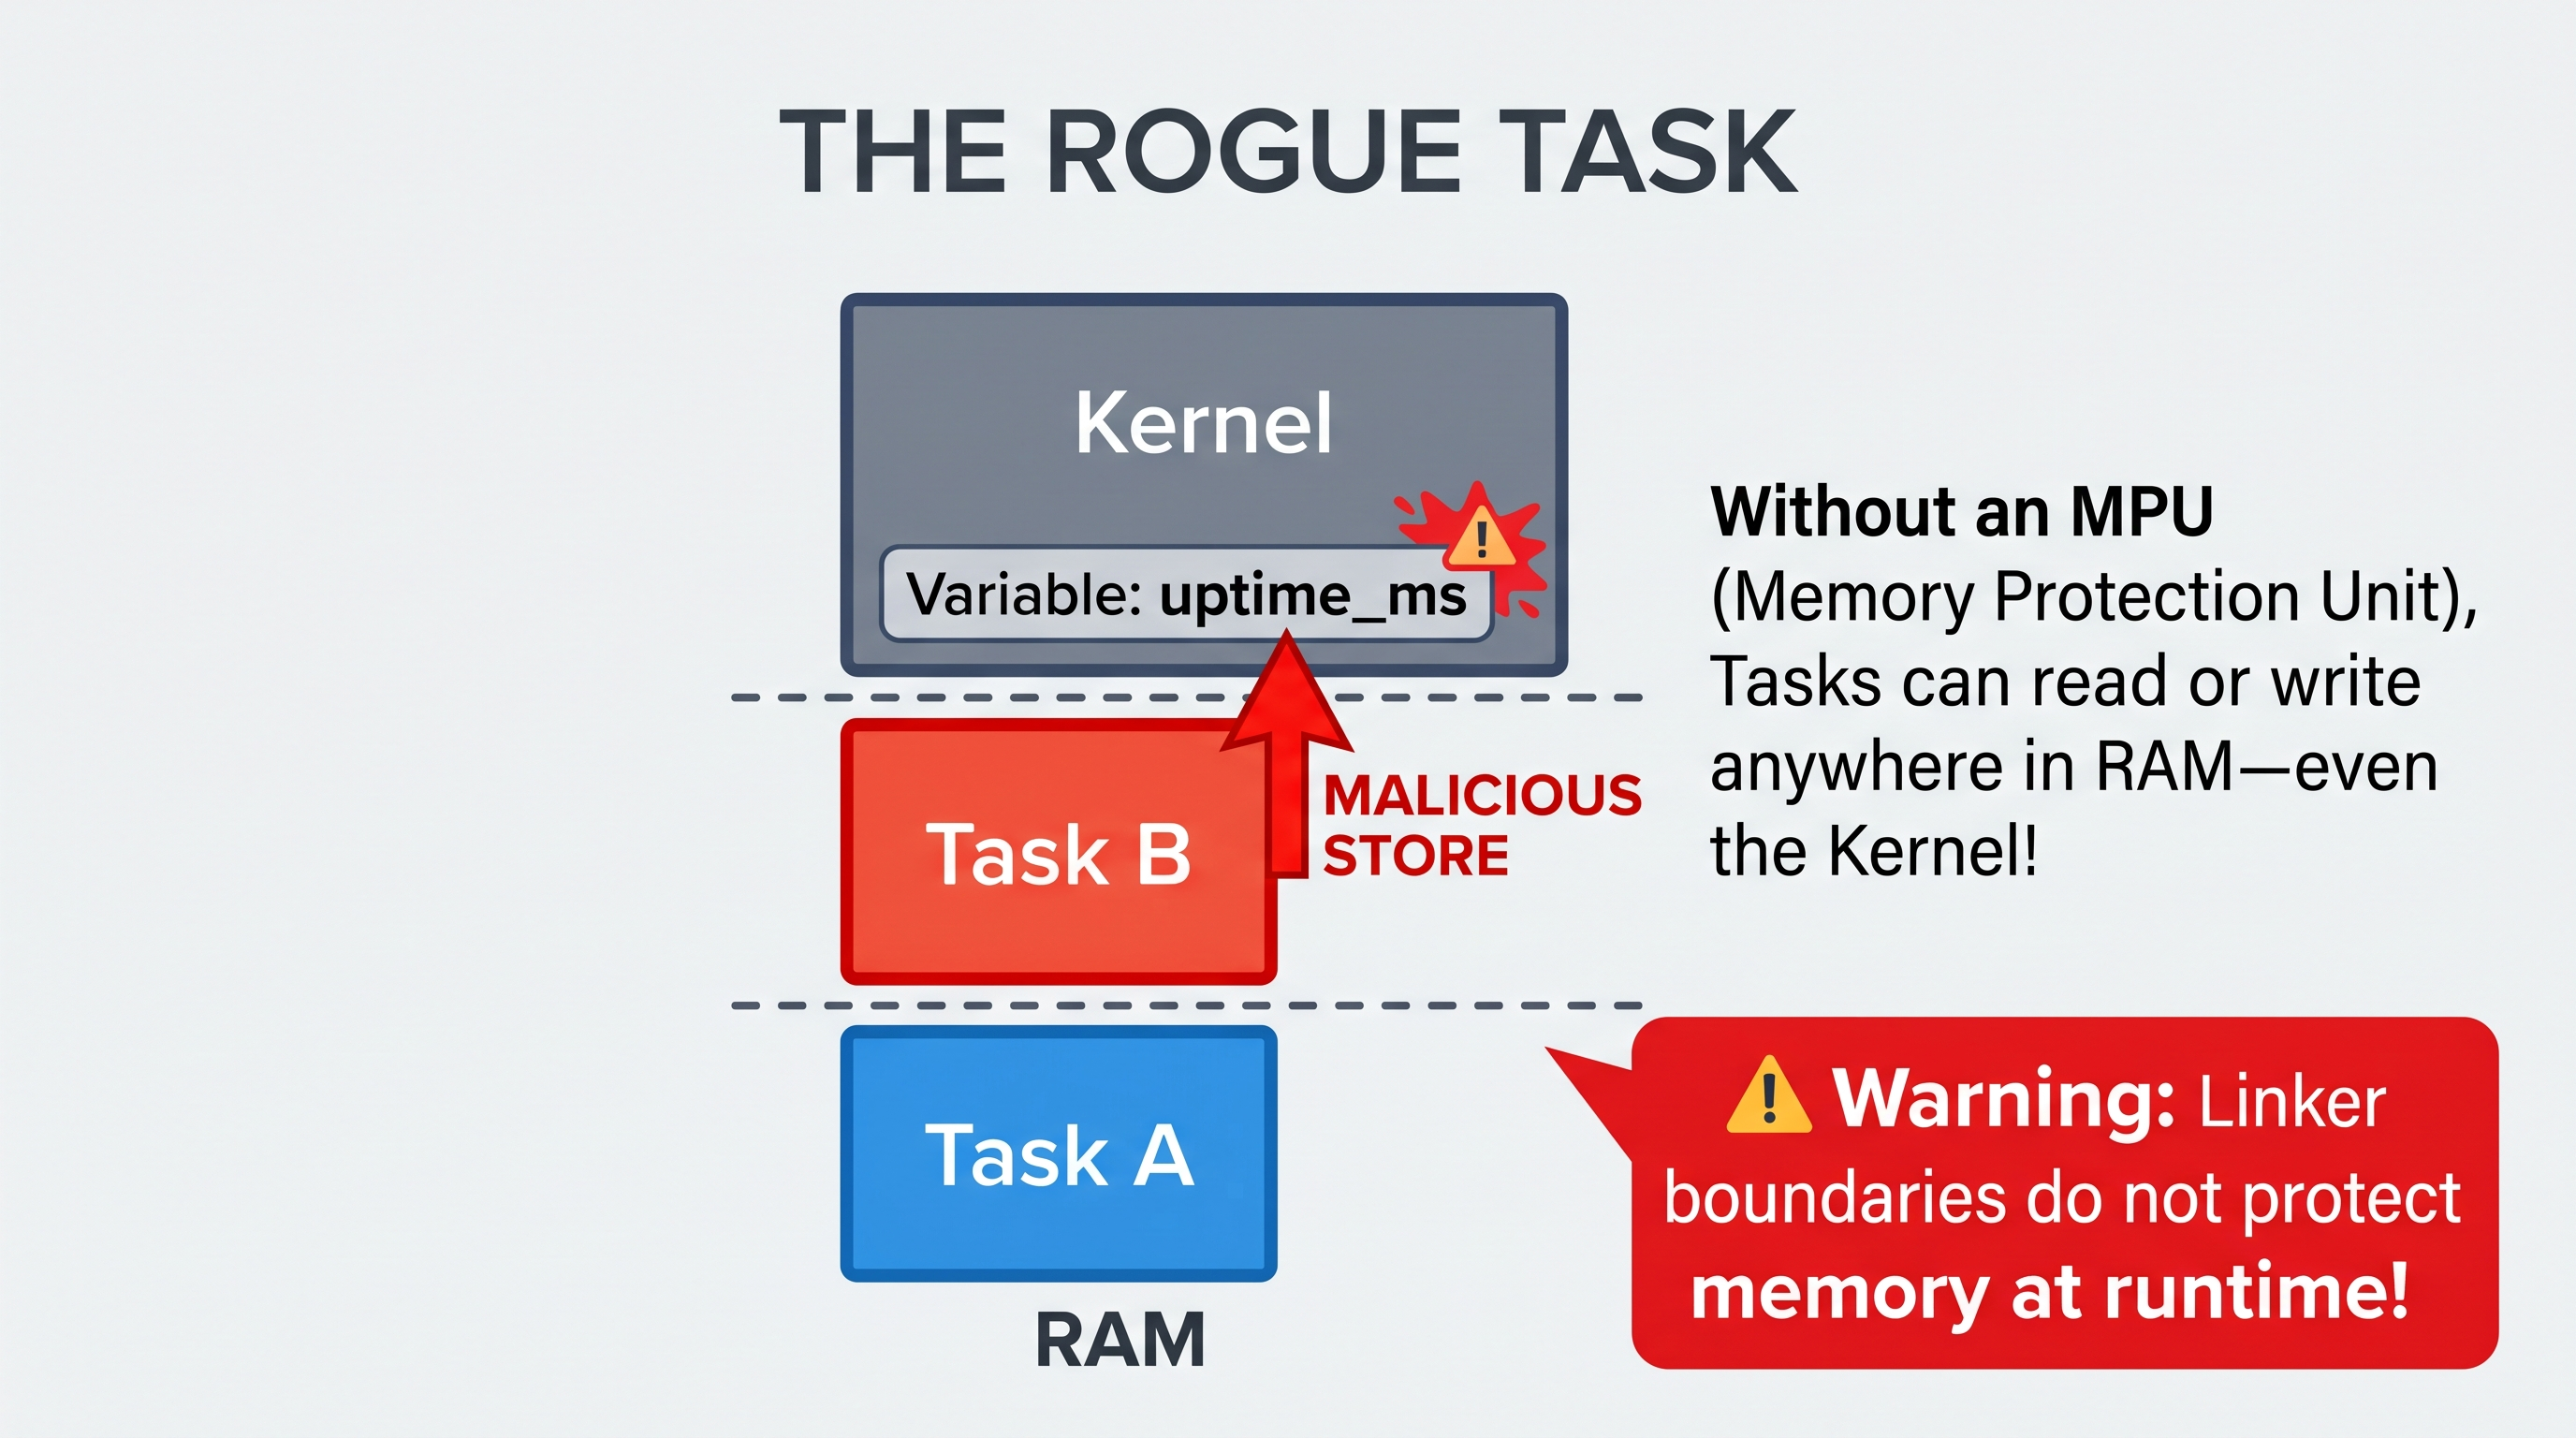
\includegraphics[width=0.5\textwidth]{contents/images/week-04/rogue_task.png}
    \caption{Importanza di proteggere la memoria -> accesso non autorizzato}
\end{figure}

\paragraph*{L'idea: una fetta di RAM per ogni task}
Una partizione contiene solo stack e variabili di un task; la FLASH conserva codice, dati in sola lettura e valori iniziali delle variabili. Cinque regole, ognuna con la sua ragione:

\begin{figure}[h]
    \centering
    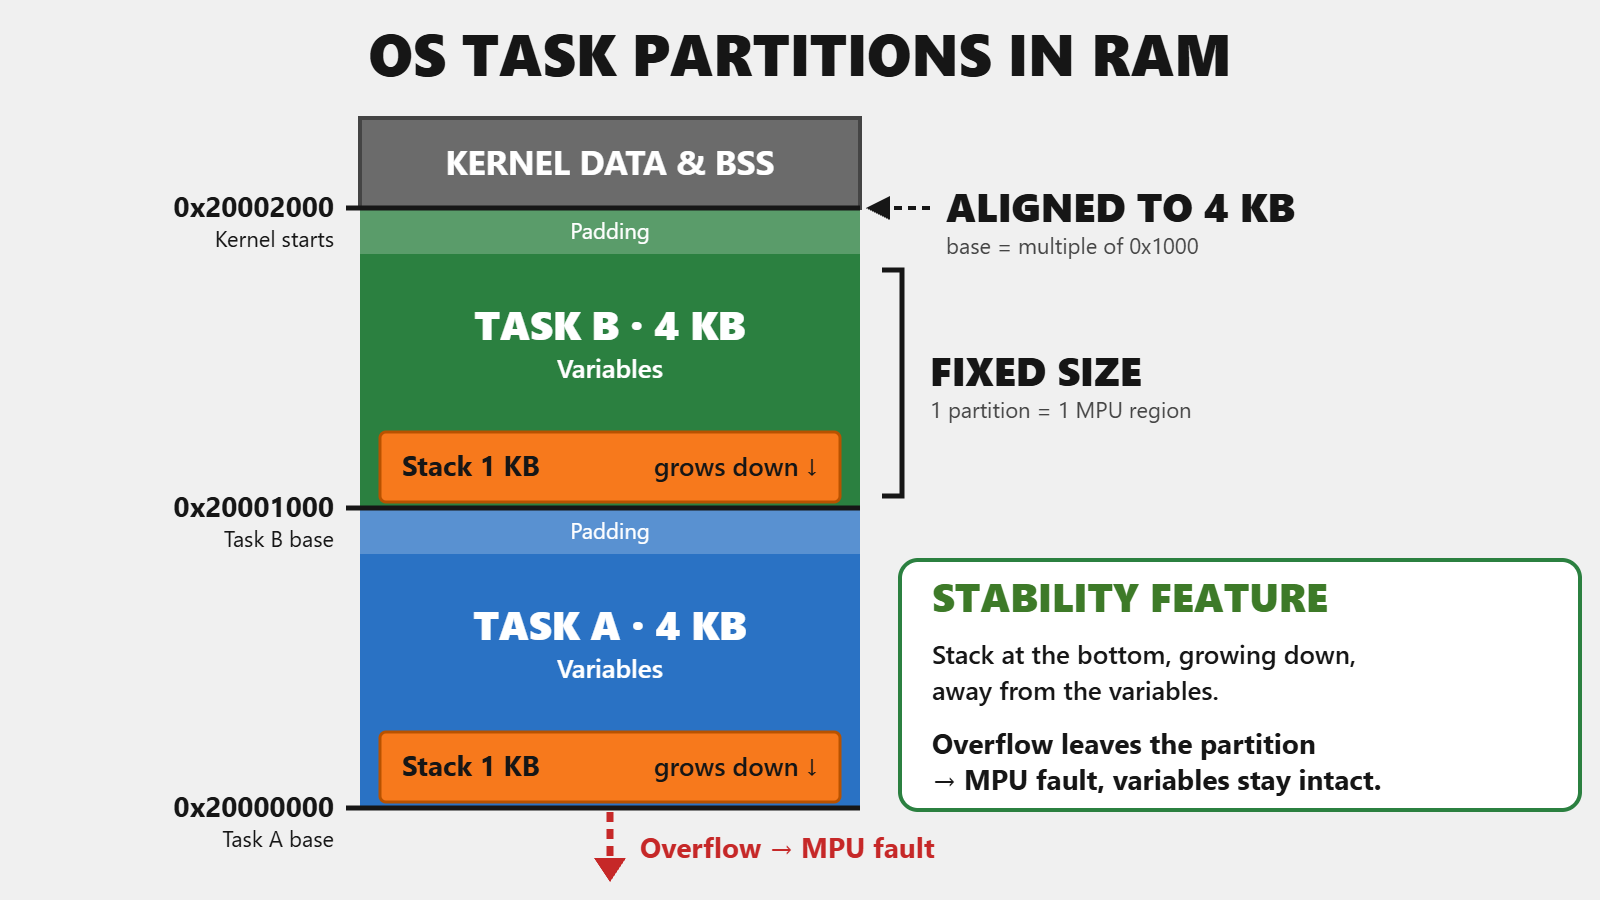
\includegraphics[width=0.5\textwidth]{contents/images/week-04/Task_partitions_in_RAM.png}
    \caption{Come la memoria viene divisa staticamente (IMPORTANTE: ancora vulnerabile a run-time)}
\end{figure}

\begin{itemize}
    \item \textbf{Fisse}: le decide il linker (allocazione statica dell'Unità 1); nessun task viene creato, ingrandito o spostato a run time.
    \item \textbf{4~KB allineate a 4~KB}: dimensione potenza di due e inizio multiplo di 4096 sono la forma che la MPU dell'Unità 3 sa proteggere; il prezzo è lo spreco (un task da 1,1~KB occupa comunque 4~KB).
    \item \textbf{Solo RAM}: codice e dati read-only restano in FLASH, \emph{condivisi} da kernel e task (una sola copia di \texttt{printf} per tutti).
    \item \textbf{Stack in fondo}: lo stack cresce verso il basso, quindi un overflow esce subito dalla partizione e l'Unità 3 potrà farlo scattare come fault; in cima, invece, sovrascriverebbe in silenzio le variabili del task, e nessuna protezione hardware distinguerebbe quella scrittura da una legittima.
    \item \textbf{Al kernel il resto}: i suoi \texttt{.data} e \texttt{.bss} seguono le partizioni e il suo stack resta in cima alla RAM.
\end{itemize}

\paragraph*{Il linker costruisce le partizioni}
Il linker usa pochi concetti. Ogni sezione ha un indirizzo di \textbf{esecuzione} (VMA), dove il codice la usa, e uno di \textbf{caricamento} (LMA), dove i suoi byte sono salvati nell'immagine. Per i dati differiscono: le variabili \emph{vivono} in RAM, ma i valori iniziali sono \emph{salvati} in FLASH, che li conserva senza alimentazione (\texttt{> RAM AT > FLASH}, come per il \texttt{.data} della Settimana 2), e qualcuno deve copiarli: il \texttt{Reset\_Handler} per il kernel, il kernel stesso per le partizioni.

\texttt{NOLOAD} riserva indirizzi senza salvare nulla (stack e padding); \texttt{ALIGN} arrotonda per eccesso a un multiplo di 4~KB; assegnare il \emph{location counter} permette di saltare a fine partizione; un pattern come \texttt{*task\_a.o(\dots)} preleva le variabili di un solo file oggetto, senza marcare il sorgente. Anche \texttt{.bss} entra nella stessa sezione dei dati, così i suoi zeri sono in FLASH e un solo ciclo di copia inizializza tutto. Vale infine il \textbf{primo match}: le regole delle partizioni vanno prima di quelle generiche del kernel, altrimenti le variabili dei task resterebbero nella RAM del kernel.

\begin{figure}[h]
    \centering
    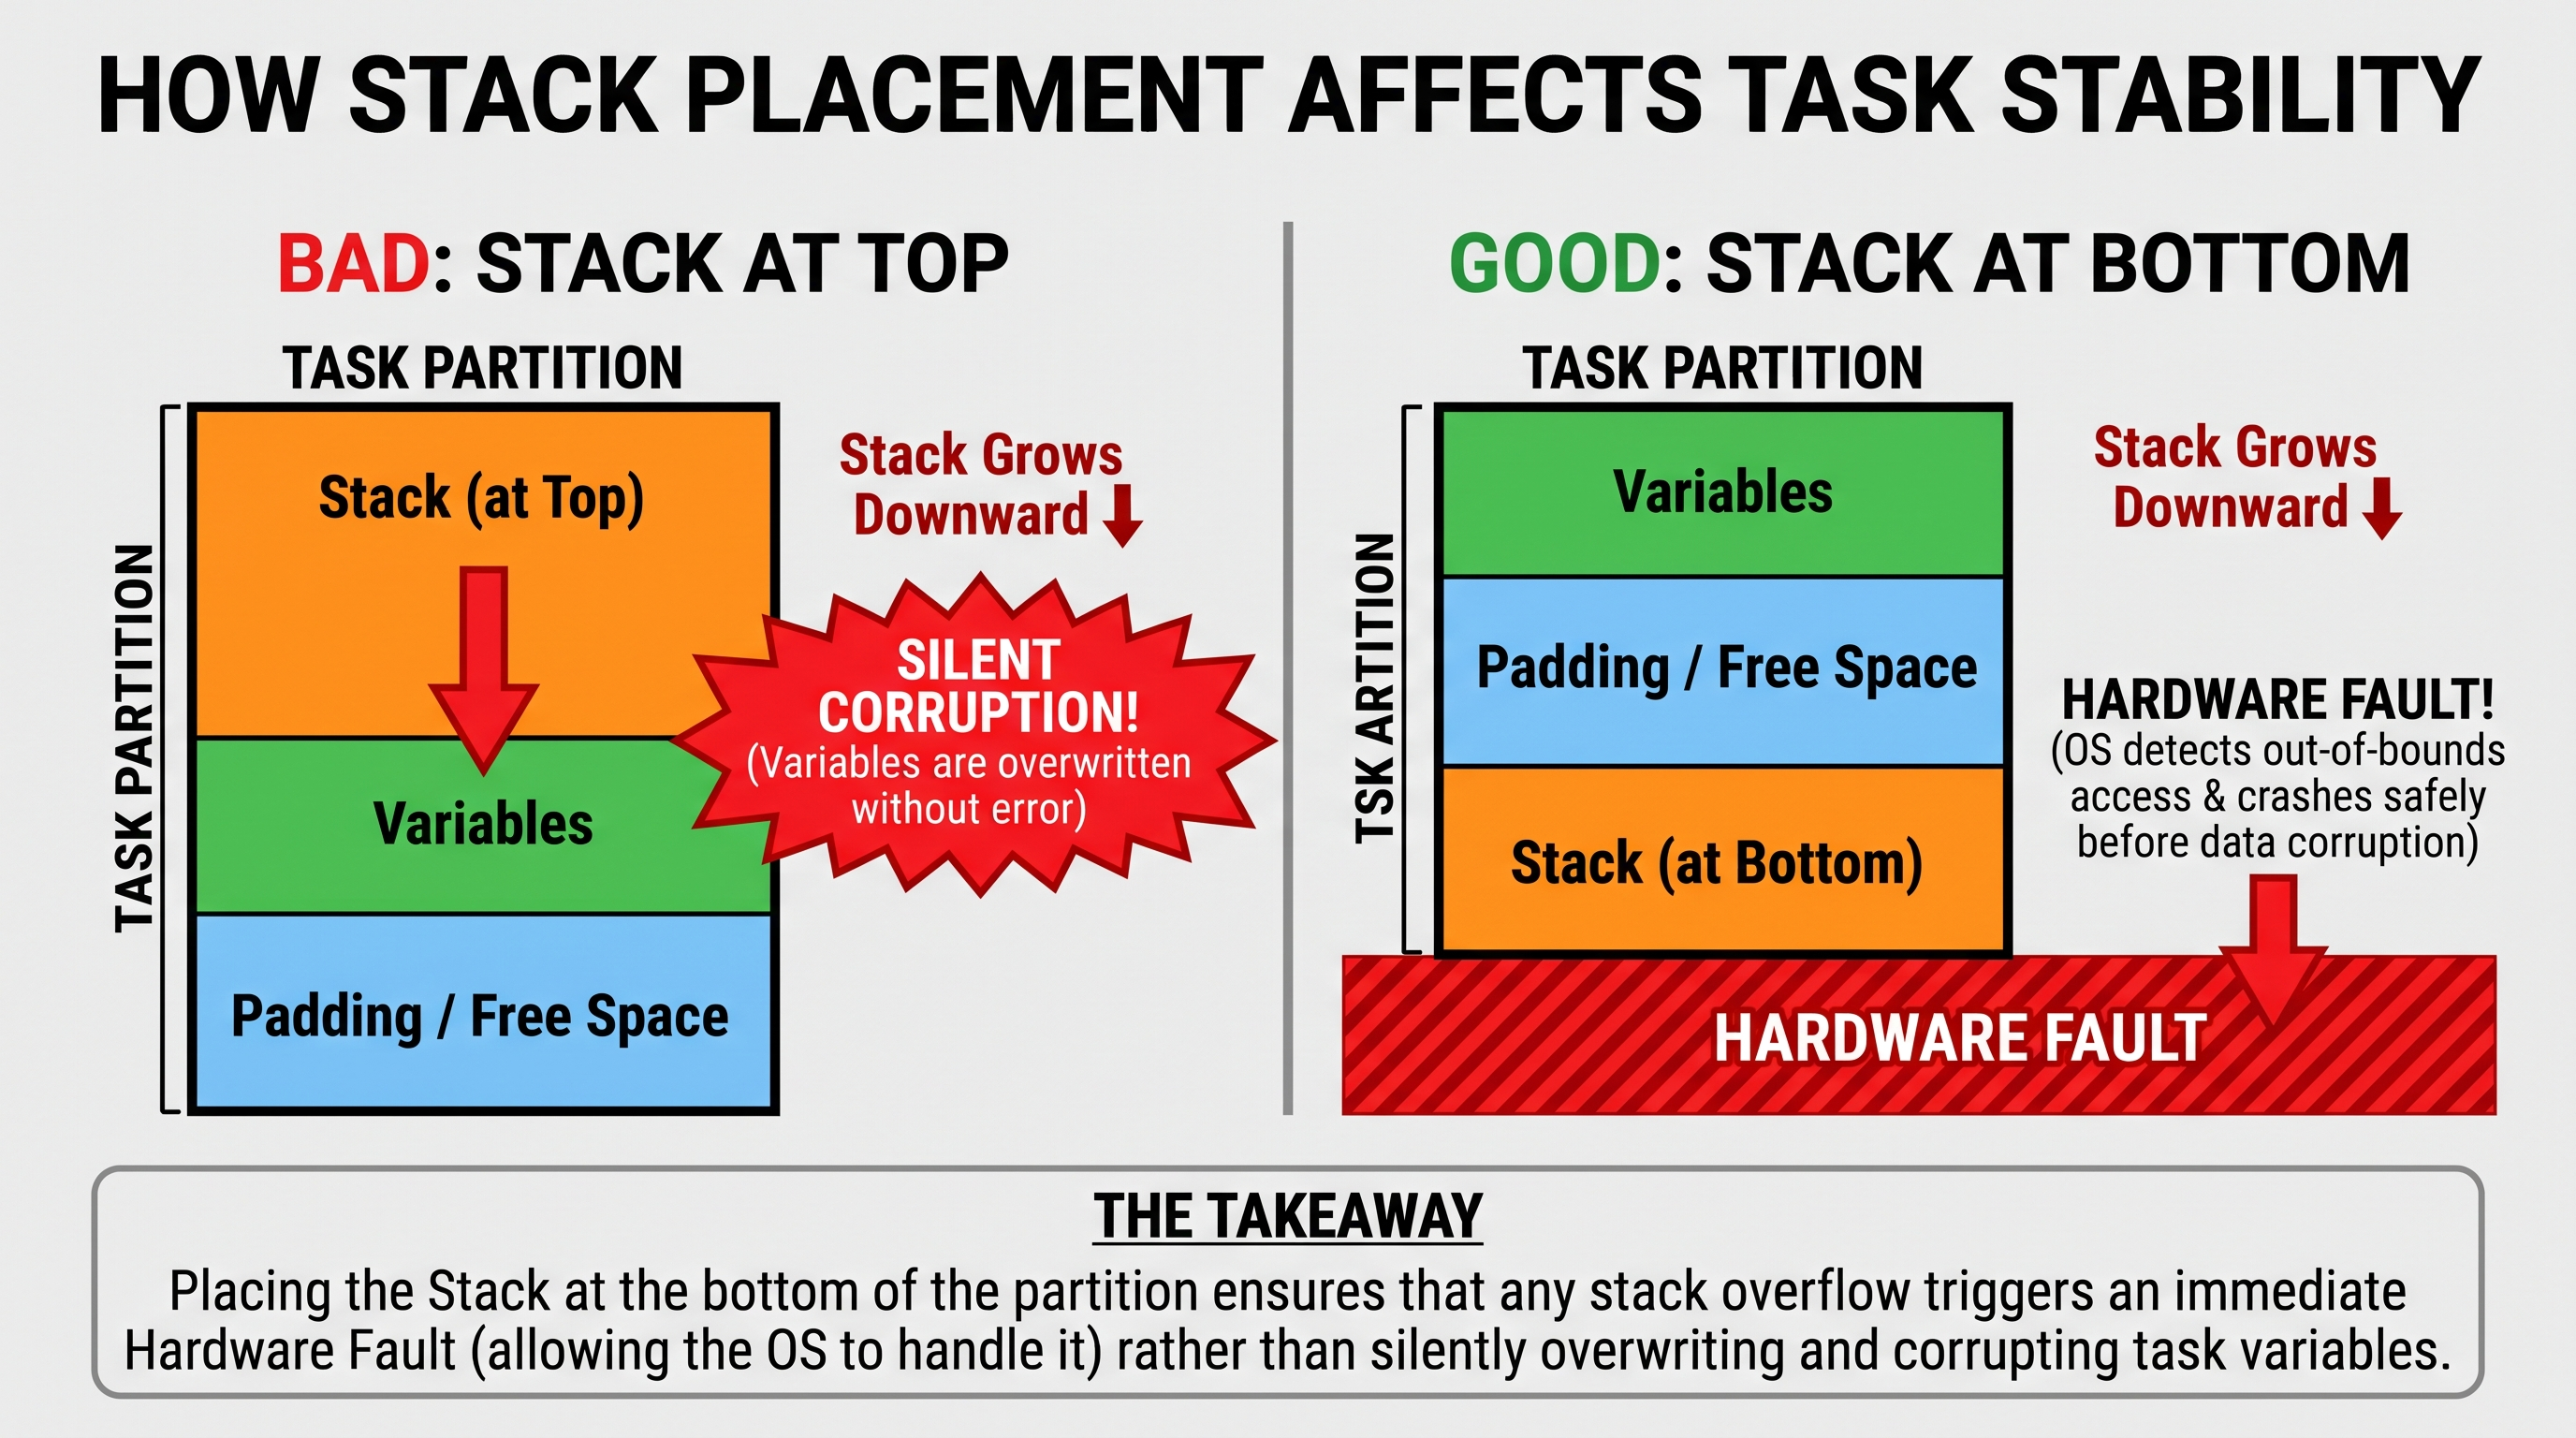
\includegraphics[width=0.5\textwidth]{contents/images/week-04/fake_stack.png}
    \caption{Importanza di uno stack alla fine di ogni partizione -> Silent Corruption}
\end{figure}

Nello script si definisce la dimensione della partizione, si elimina la vecchia sezione piatta degli stack e si inserisce, prima di \texttt{.data}, il blocco di A seguito da quello di B. Ogni blocco ha tre sezioni: \textbf{stack} (parte dal primo confine da 4~KB, riserva 1~KB e ne segna la cima), \textbf{dati} (le variabili del file del task, con estremi allineati alla word perché la copia procede per word da 32 bit) e \textbf{padding} (porta il location counter a fine partizione, così la successiva parte dopo i 4~KB completi). Per A l'allineamento parte dall'inizio della RAM, perché dopo \texttt{.text} il location counter è ancora in FLASH. I sei simboli per task già usati dal kernel vengono solo \emph{ri-puntati}, e due \texttt{ASSERT} fanno fallire il link se i dati di un task non stanno nella sua partizione.
Con \texttt{nm} si verifica il risultato: due blocchi consecutivi da 4~KB allineati, con lo stack nel primo KB, e i dati del kernel spostati dopo di essi. La cima dello stack coincide con l'indirizzo della prima variabile senza sovrapporsi: è un limite \emph{esclusivo}, perché lo stack del Cortex-M è \emph{full descending} (un push prima decrementa \texttt{sp}, poi scrive). Il map file conferma il primo match.

\paragraph*{Inizializzare le variabili dei task}
Il linker decide dove stanno le variabili, ma non dà loro un valore: girano in RAM e nascono in FLASH. Per questo \texttt{partition\_init} le copia, una word alla volta, prima della prima esecuzione di ogni task: è lo stesso ciclo con cui il \texttt{Reset\_Handler} inizializza i dati del kernel, lanciato da \texttt{task\_launch} una volta per task. Una \texttt{struct task} raccoglie ciò che il kernel sa di ogni task (nome, funzione d'ingresso, stack, confini della partizione, indirizzi dei dati) ed è riempita con i simboli del linker, dichiarati come array perché conta solo il loro indirizzo. Per \texttt{.bss} non serve azzerare nulla: gli zeri sono già nella sezione caricata. Nella versione di base il ciclo non copiava niente, così il codice preparato girava subito.

\begin{figure}[h]
    \centering
    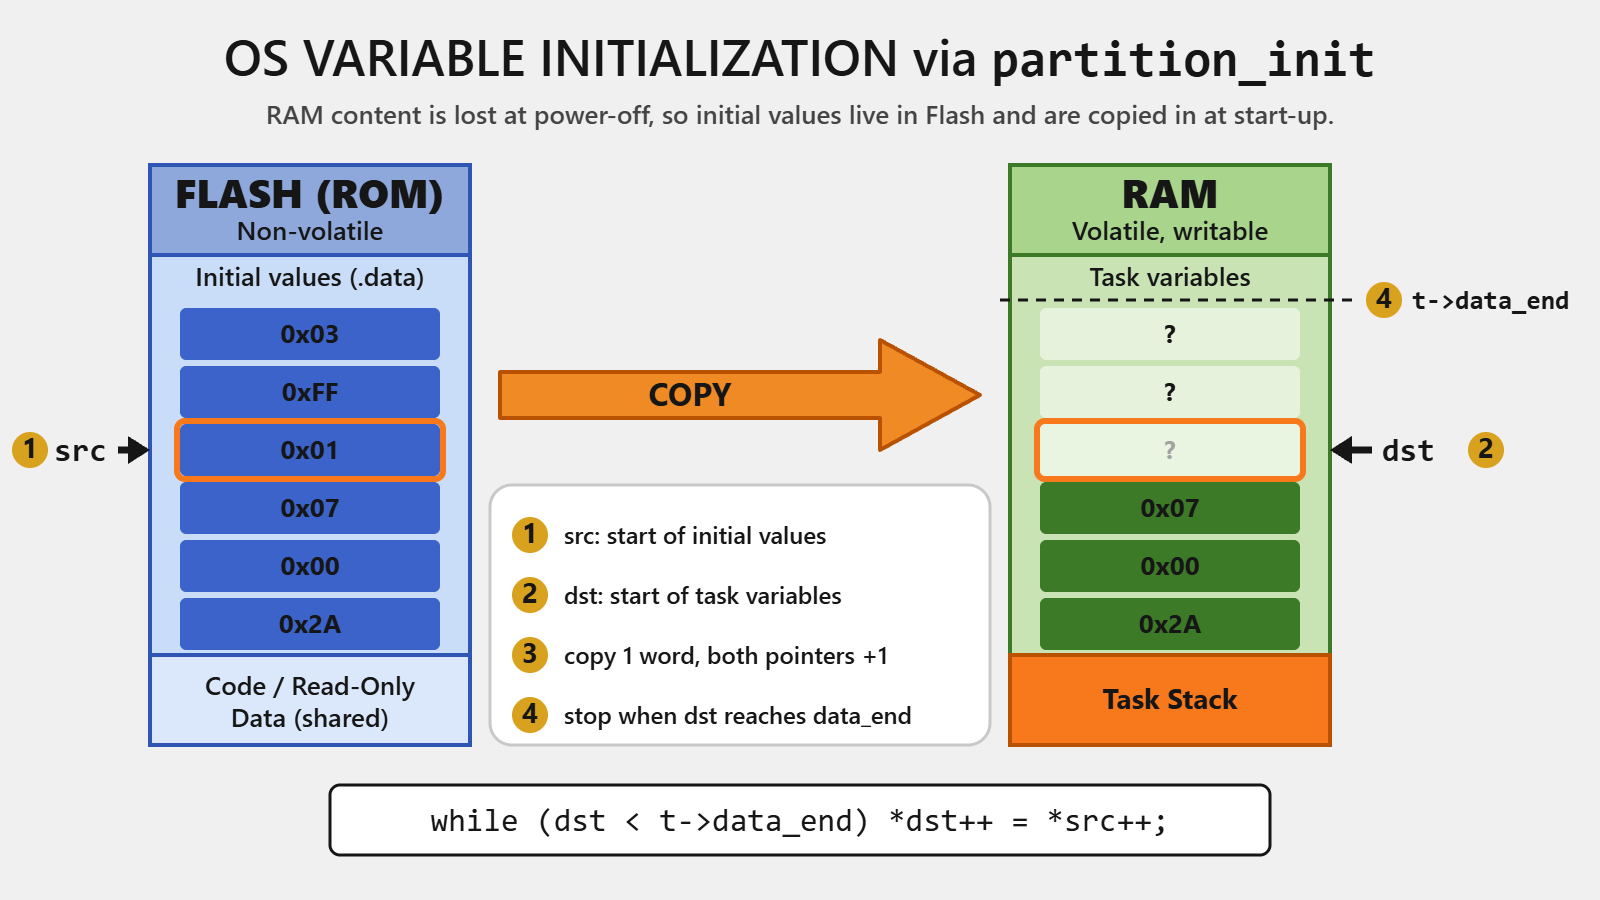
\includegraphics[width=0.5\textwidth]{contents/images/week-04/partition_init.png}
    \caption{Partition Init}
\end{figure}

\paragraph*{Due stack, due livelli di privilegio}
Il passo successivo è separare stack e privilegi. Il Cortex-M3 ha due stack pointer, e \texttt{sp} è quello in uso. \textbf{MSP} (main) è sempre usato in \emph{handler mode}, e in thread mode dopo il reset: è lo stack del kernel, in cima alla RAM. \textbf{PSP} (process) è usato in thread mode quando il bit SPSEL di CONTROL vale 1: ogni task ha il suo stack PSP \emph{dentro} la propria partizione. Se nPRIV vale 1 il thread mode è non privilegiato, quindi un task gira con \textbf{CONTROL = 3}. Lo stack deve stare nella partizione perché contiene variabili locali, indirizzi di ritorno e frame delle eccezioni: altrimenti non si potrebbe confinare il task nei suoi 4~KB senza togliergli lo stack. 

\begin{figure}[h]
    \centering
    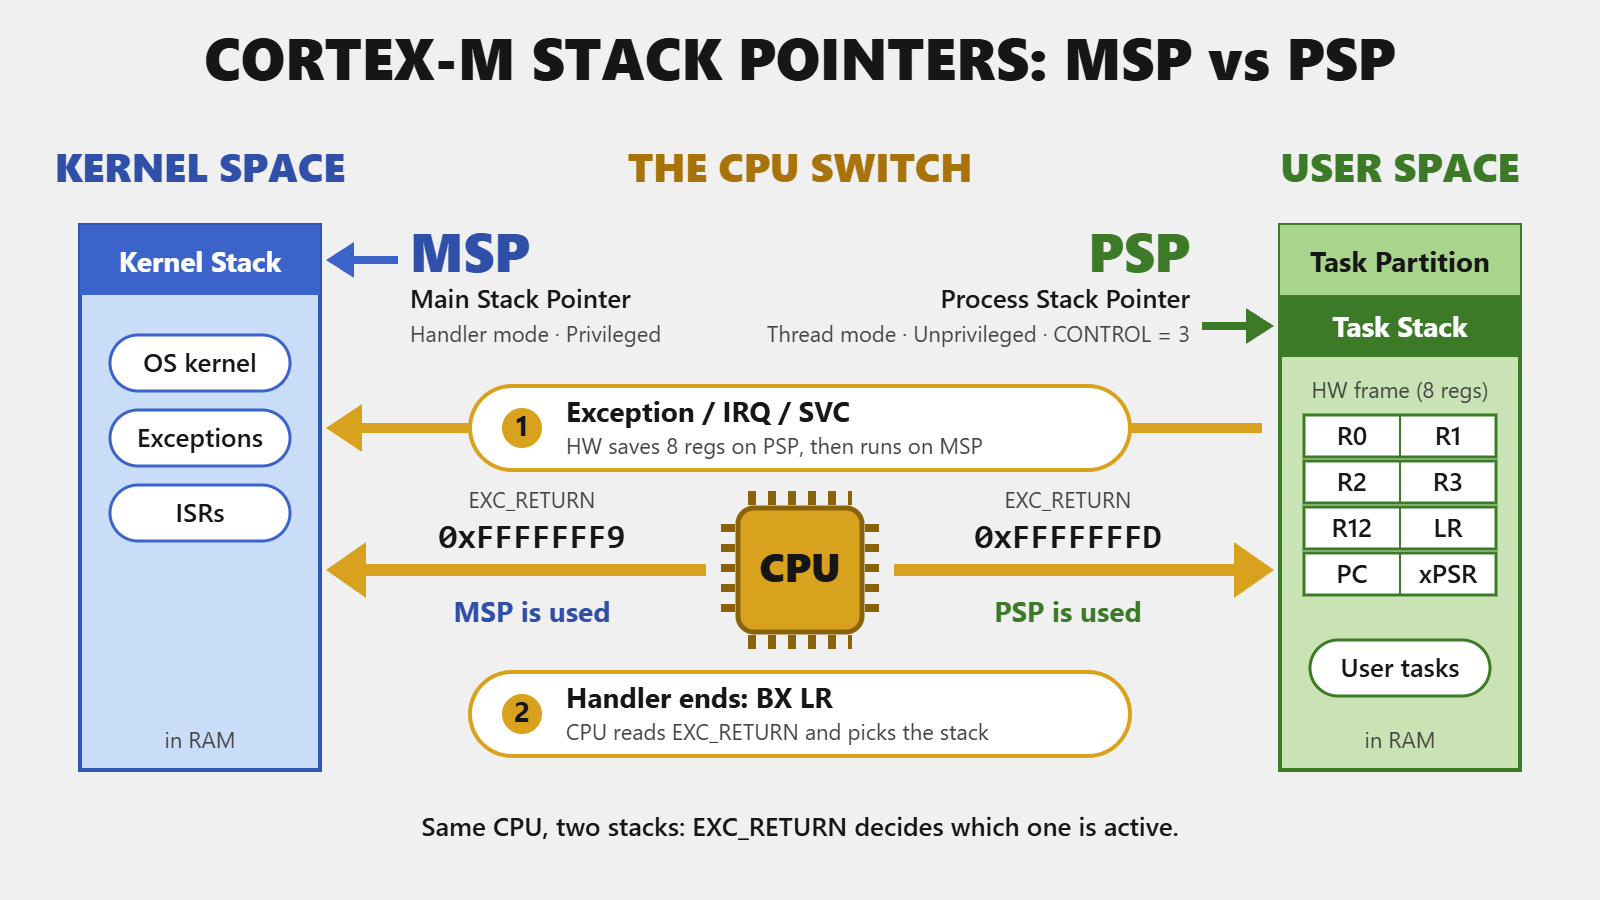
\includegraphics[width=0.5\textwidth]{contents/images/week-04/MSP_vs_PSP_2.png}
    \caption{MSP \& PSP - Exception Return}
\end{figure}

E poiché l'handler mode usa sempre MSP, il lavoro del kernel non passa mai dallo stack di un task. Il ponte tra i due mondi è \textbf{EXC\_RETURN}, il valore in \texttt{lr} che chiude un'eccezione: \texttt{0xFFFFFFF9} torna in thread mode su MSP, \texttt{0xFFFFFFFD} su PSP. All'ingresso in un'eccezione l'hardware ne mette uno in \texttt{lr}, e il suo bit 2 indica dove sta il frame salvato (1 = PSP, 0 = MSP).

\paragraph*{Avviare un task: il frame finto}
Resta da far partire un task. Il kernel opera in handler mode, su MSP e con tutti i privilegi: una normale chiamata di funzione farebbe ereditare questo stato al task, e un suo bug potrebbe corrompere il kernel. Il task deve invece girare in thread mode, non privilegiato e su PSP. Ma nessuna istruzione cambia insieme stack, privilegi, modalità e indirizzo: solo l'\textbf{exception return} compie questo ``triplo salto'' in modo sicuro e atomico. Un task appena creato, però, non è mai stato interrotto: il kernel \emph{finge} allora il passato, costruendo sul suo stack un frame di 8 word (32 byte) identico a quello che l'hardware si aspetta, puntando il PSP a quel frame e ordinando il ritorno con \texttt{0xFFFFFFFD}. La CPU non si accorge dell'inganno: ripristina i registri, abbassa i privilegi, passa in thread mode e salta all'indirizzo iniziale del task.

\begin{figure}[h]
    \centering
    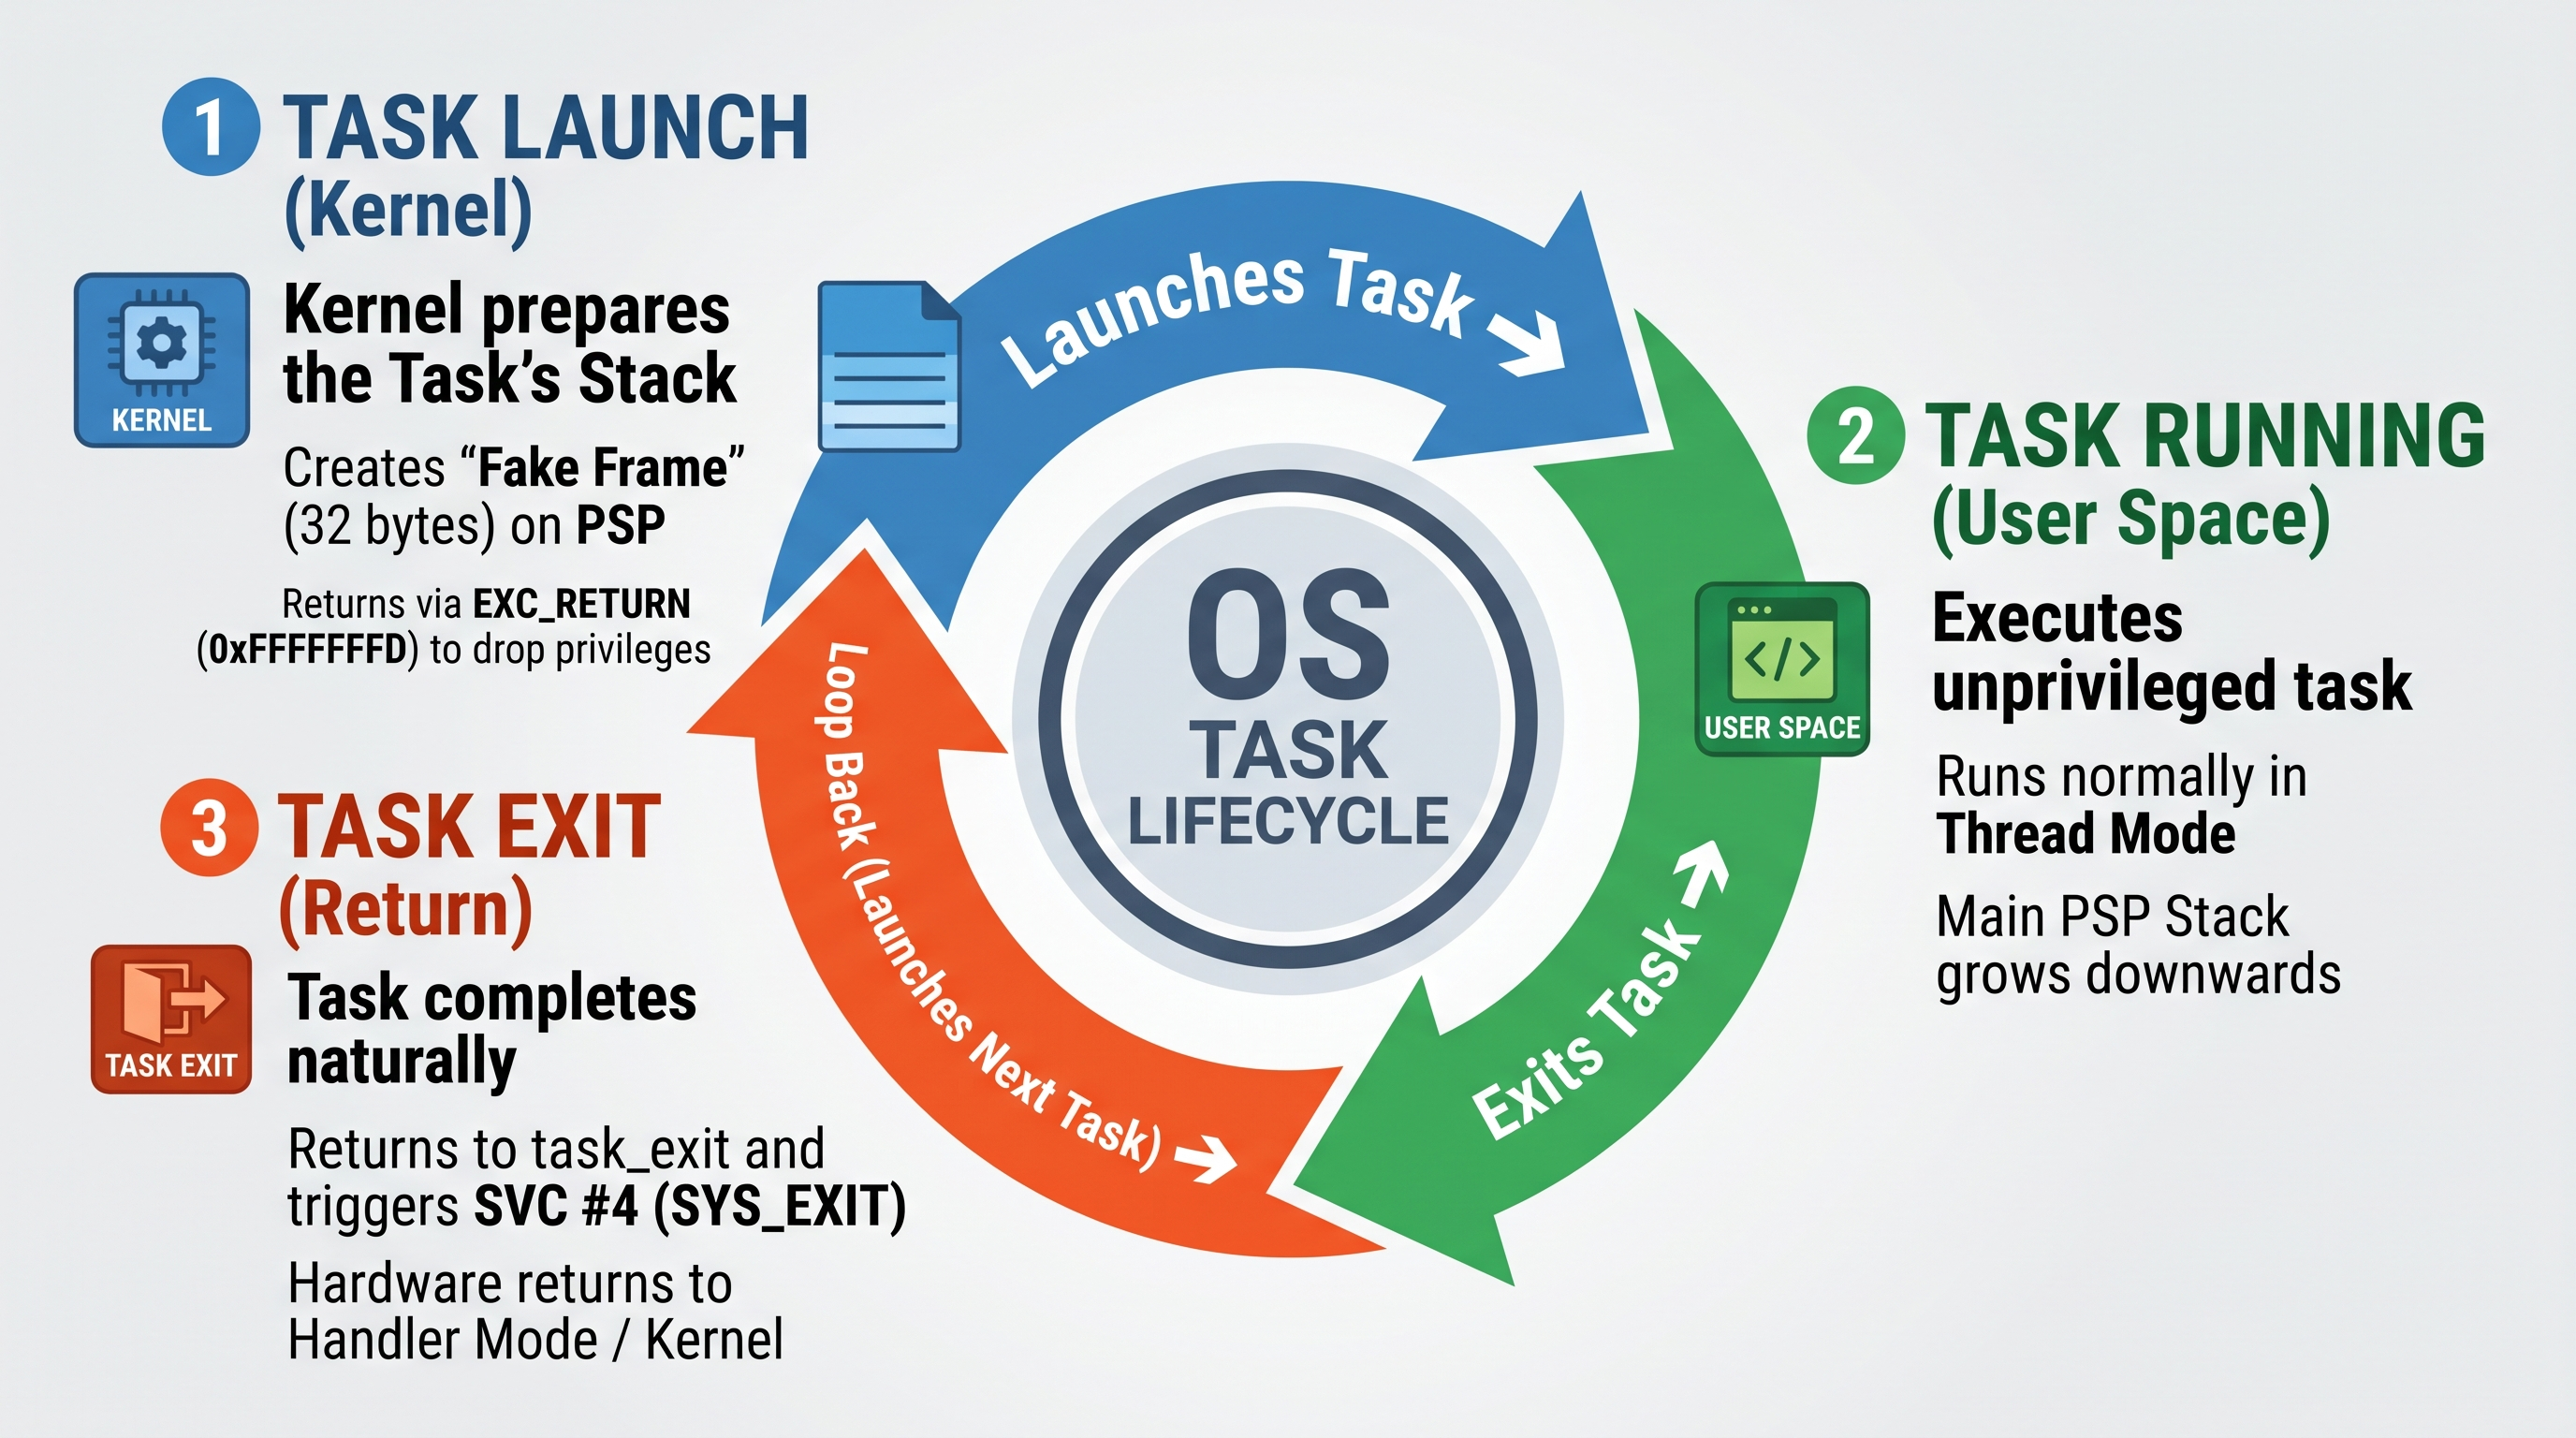
\includegraphics[width=0.5\textwidth]{contents/images/week-04/task_lifestyle.png}
    \caption{Ciclo di vita di un task (gestito dal OS)}
\end{figure}

La sequenza parte da \texttt{main} con la system call di avvio; l'handler intercetta la chiamata e fa partire \texttt{task\_launch}, che compie tre operazioni. Prima la \emph{preparazione}: registra quale task parte, predispone la MPU a proteggerne la partizione e chiama \texttt{partition\_init}. Poi costruisce il \emph{frame} sotto la cima dello stack: \texttt{r0--r3} e \texttt{r12} a zero, \texttt{lr} = \texttt{task\_exit} (se la funzione del task ritorna, il task esce in modo pulito invece di andare in crash), \texttt{pc} = punto d'ingresso, \texttt{xPSR} con il bit Thumb, obbligatorio sul Cortex-M (senza, scatta una \texttt{UsageFault}). Infine il \emph{cambio di contesto}, in assembly: carica il frame nel PSP, attiva nPRIV in CONTROL e forza il ritorno di \texttt{0xFFFFFFFD}. L'hardware estrae i 32 byte e il task parte non privilegiato, con il PSP, liberato dal frame, esattamente in cima allo stack.

\paragraph*{System call e fine di un task}
Ora una \texttt{svc} può arrivare da due ambienti: da \texttt{main}, una sola volta per avviare il sistema (su MSP), e dai task, per le chiamate ordinarie (su PSP). L'\texttt{SVC\_Handler} deve quindi scoprire dove sta il frame, e lo fa leggendo il bit 2 dell'EXC\_RETURN in \texttt{lr}: 0 = MSP, 1 = PSP. In assembly sceglie lo stack giusto e chiama la funzione C \texttt{svc\_dispatch}, passandole frame ed EXC\_RETURN; il valore restituito è un nuovo EXC\_RETURN, con cui l'assembly esce dall'eccezione. Prima l'handler tornava sempre al punto di chiamata; ora è \texttt{svc\_dispatch} a decidere \emph{dove tornare}. Con \texttt{SYS\_START\_TASKS} restituisce il codice per lanciare il primo task (\texttt{task\_start\_first}); con \texttt{SYS\_EXIT} quello per lanciare il successivo o tornare a \texttt{main} (\texttt{task\_exit\_current}); per le chiamate normali scrive il risultato in \texttt{frame[0]} (che diventa \texttt{r0} del task) e restituisce l'EXC\_RETURN originale, così l'esecuzione riprende da dove si era interrotta. È la regola d'oro: \textbf{il kernel non aspetta mai dentro un handler}; ogni system call finisce subito e guida la CPU verso ciò che deve girare dopo.

\begin{figure}[h]
    \centering
    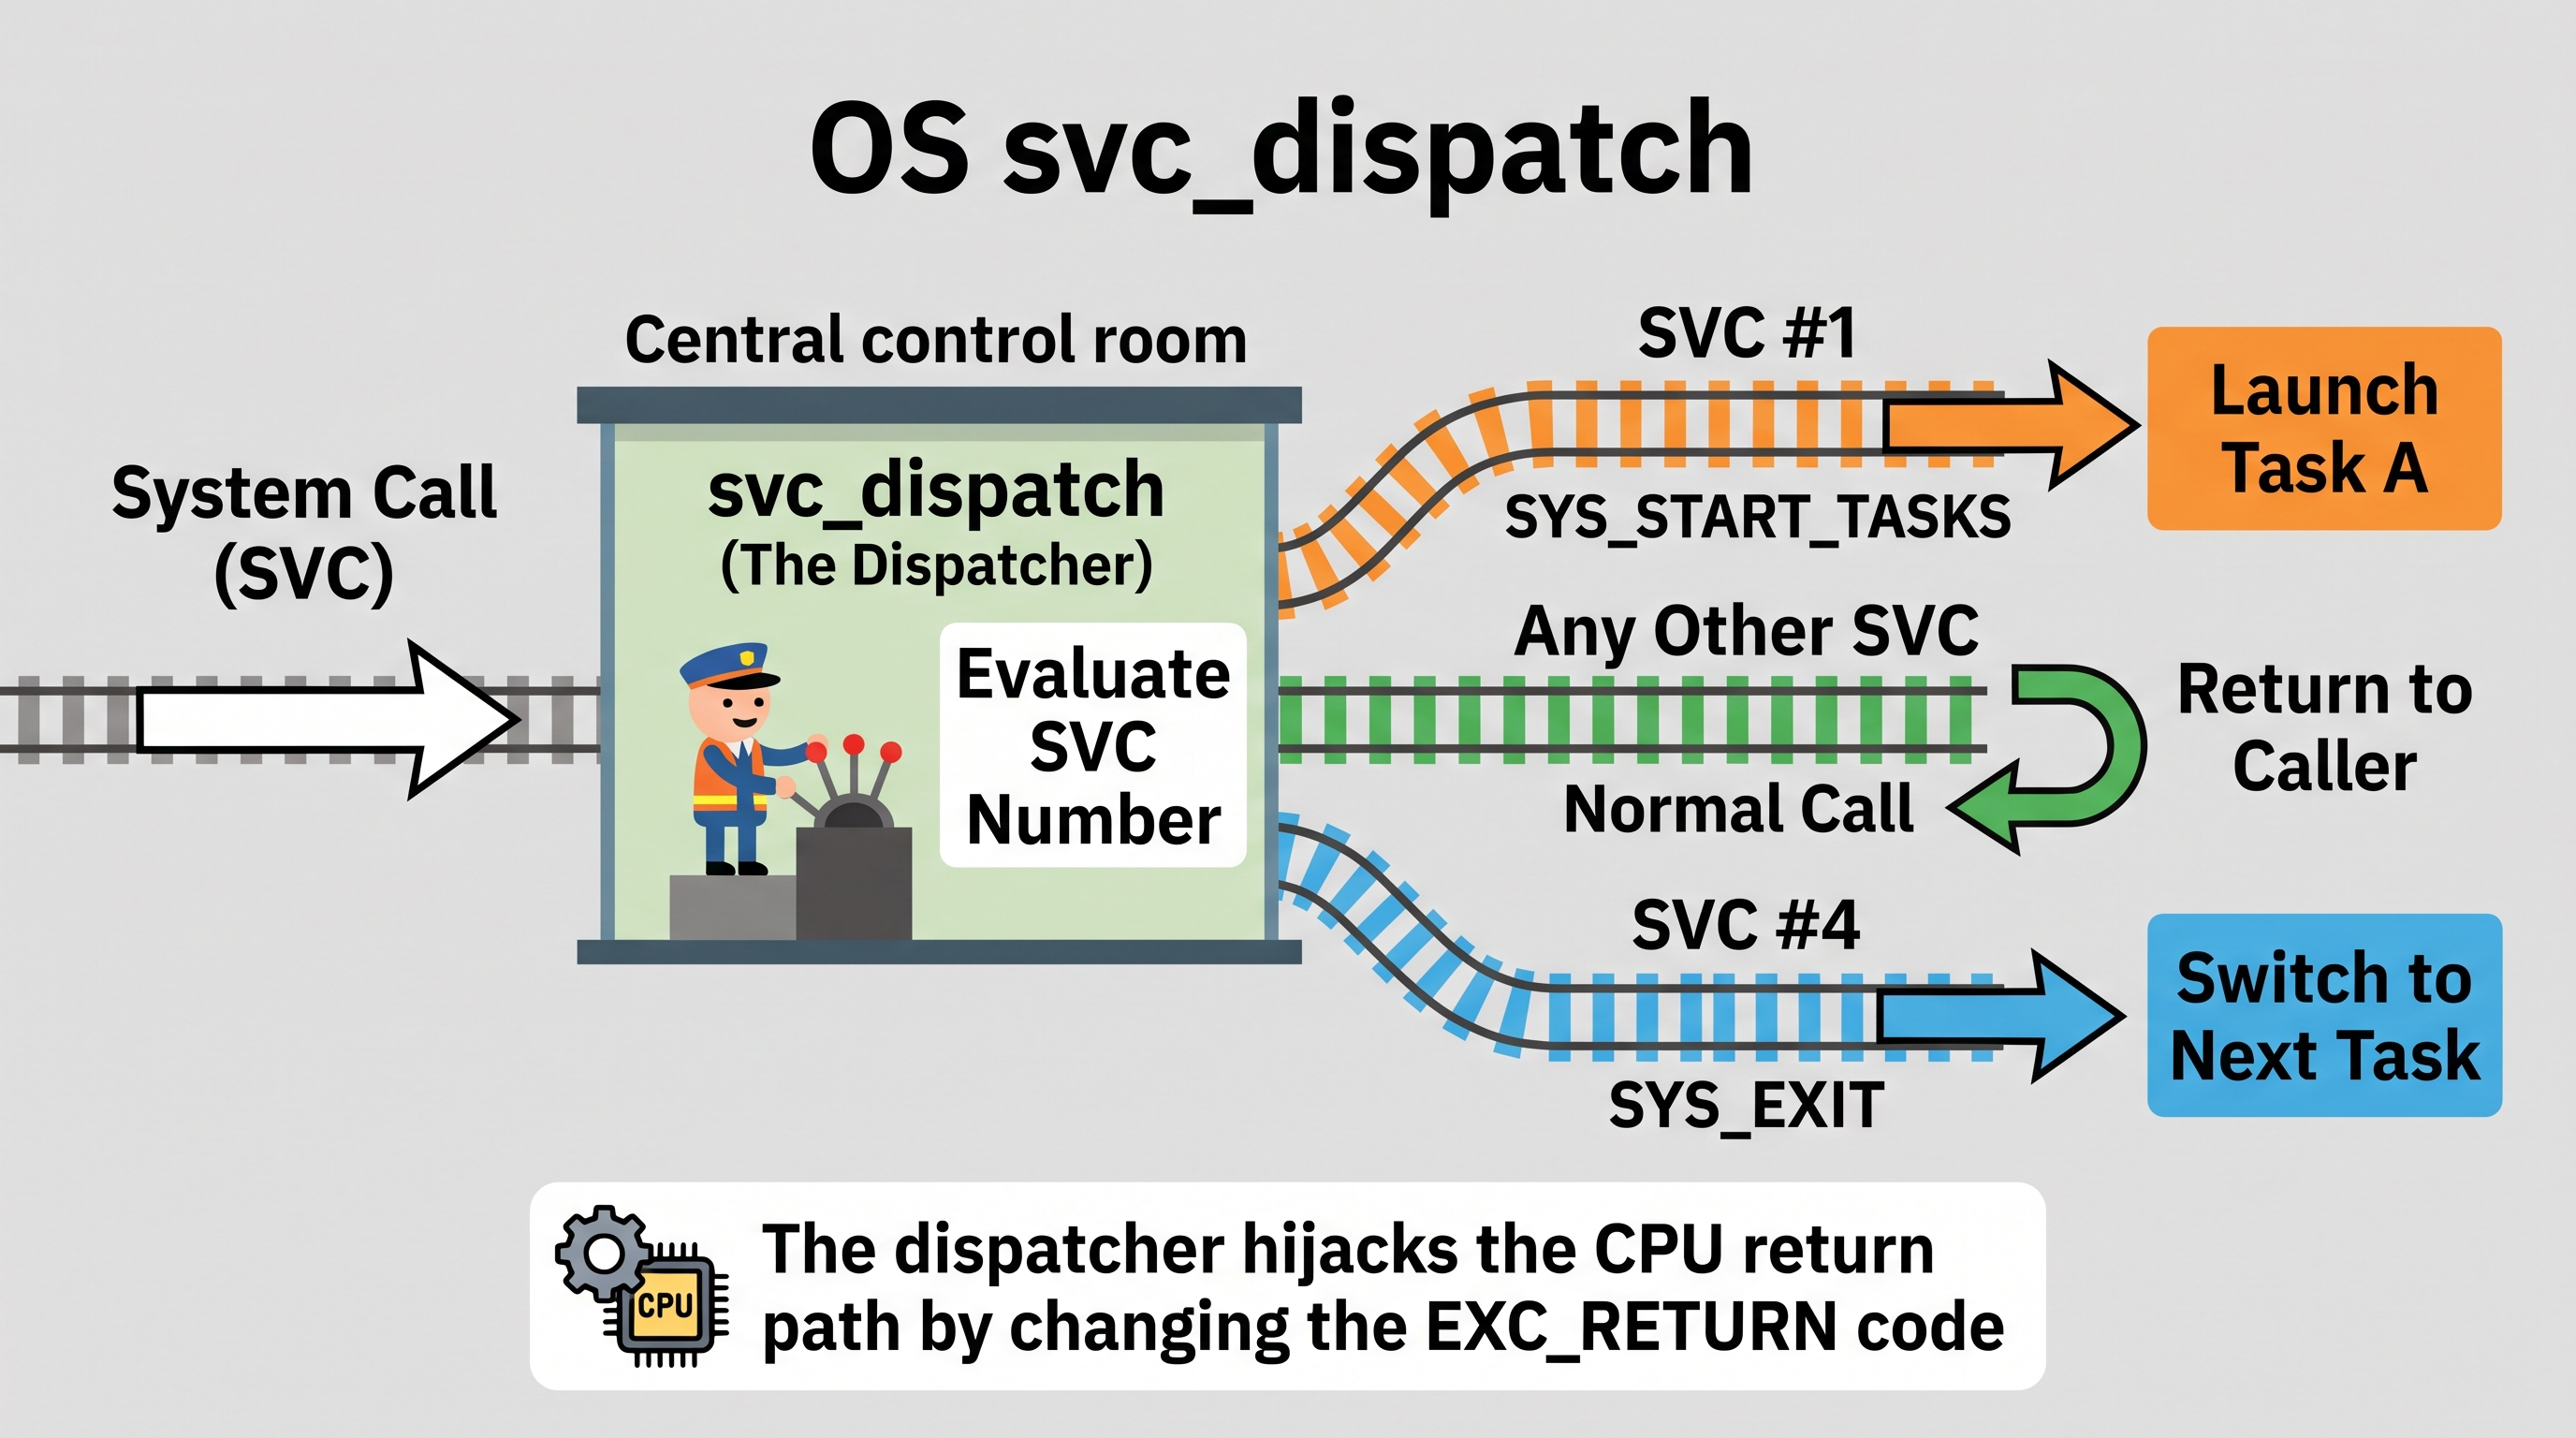
\includegraphics[width=0.5\textwidth]{contents/images/week-04/dispatcher.png}
    \caption{Opzioni di un dispatcher}
\end{figure}

Un task può terminare chiamando \texttt{sys\_exit()}, uno stub che non ritorna mai, oppure semplicemente ritornando dalla sua funzione: atterra così in \texttt{task\_exit}, l'indirizzo che \texttt{task\_launch} ha messo nel \texttt{lr} del frame finto, che a sua volta chiama \texttt{sys\_exit}. Il Task A usa questa seconda strada. Il frame finto, quindi, non solo avvia il task ma ne prepara anche l'uscita; il lato kernel si vedrà nell'Unità 3.

\paragraph*{Verifiche e limite delle partizioni}
Con \texttt{gdb} si controlla la catena: in entrambi i task \textbf{CONTROL = 3}; il \textbf{PSP} coincide con la cima dello stack, dentro la partizione del task; il frame mostra \texttt{lr} = \texttt{task\_exit} (più il bit Thumb), \texttt{pc} = funzione del task e \texttt{xPSR} con il bit Thumb; l'\textbf{MSP} è lo stesso nei due casi, perché contiene il frame di \texttt{main} in attesa e i task non lo toccano mai.

Eppure, rieseguendo la demo \emph{rogue}, il Task B scrive ancora nella variabile del kernel (ora spostata, fuori dalla sua partizione) e l'orologio viene corrotto \emph{esattamente come nell'Unità 1}. Il linker decide solo \emph{dove} stanno le cose: una scrittura è una scrittura ordinaria e, a run time, nulla la confronta con i confini della partizione. Le partizioni \emph{dispongono} la memoria ma non \emph{impongono} nulla. È cambiata però la forma: la memoria di ogni task è ora un blocco unico da 4~KB allineato, quindi basta \emph{una} regola hardware per task per descrivere ciò che può toccare. Quella regola è la MPU, oggetto dell'Unità 3.

\paragraph*{In breve}
Partizioni fisse da 4~KB allineate, con lo stack in fondo e il codice condiviso in FLASH $\rightarrow$ costruite dal linker (\texttt{ALIGN}, \texttt{NOLOAD}, \texttt{AT > FLASH}, pattern per file, primo match, \texttt{ASSERT}) $\rightarrow$ riempite da \texttt{partition\_init} $\rightarrow$ eseguite in modo non privilegiato su PSP, con il kernel su MSP $\rightarrow$ avviate da \texttt{task\_launch} con un frame finto e \texttt{0xFFFFFFFD} $\rightarrow$ gestite nelle system call da \texttt{SVC\_Handler} e \texttt{svc\_dispatch} $\rightarrow$ chiuse da \texttt{task\_exit}. La memoria è ora \emph{organizzata}, ma non ancora \emph{difesa}: per farla rispettare serve la MPU dell'Unità 3.


\subsection{Unità 3}
L'obiettivo è impedire \textbf{via hardware} che un task esca dai propri confini. L'Unità~1 aveva
introdotto la MPU come lista di regioni controllate a ogni accesso e l'Unità~2 aveva preparato la
memoria (una partizione da 4~KB, allineata, per ogni task): ora si programma la MPU perché ogni
task veda solo la FLASH e la propria partizione, e si osserva cosa accade quando prova a uscirne.

\paragraph*{Come ragiona la MPU.}
Il Cortex-M3 ha \textbf{8 regioni}; ognuna ha \textbf{base}, \textbf{dimensione} e
\textbf{permessi} e vale solo se il suo bit ENABLE è attivo. La dimensione è una potenza di 2
tra 32~byte e 4~GB e la base deve essere un \textbf{multiplo della dimensione}: per questo
l'Unità~2 ha reso le partizioni di 4~KB e allineate a 4~KB, così che \emph{una regione copra
esattamente una partizione}. Il controllo vale per il codice \textbf{non privilegiato} (i task):
un accesso fuori da ogni regione attiva, o vietato dalla regione, viene \textbf{bloccato} e la
CPU solleva un fault MemManage. Per il codice \textbf{privilegiato} (il kernel), il bit
PRIVDEFENA decide se, dove nessuna regione corrisponde, valga la stessa regola o la mappa di
memoria predefinita della scheda. La MPU è una periferica del core scrivibile solo in modo
privilegiato, quindi un task non può spegnerla.

\paragraph*{I permessi.}
Il campo \textbf{AP} (3 bit) assegna diritti distinti al codice privilegiato e a quello non
privilegiato: qui servono lettura/scrittura per entrambi sulla partizione del task in esecuzione
e sola lettura sulla FLASH. Il bit \textbf{XN} (\emph{execute never}) vieta il \emph{fetch} di
istruzioni, mentre letture e scritture seguono AP: le partizioni contengono solo dati e stack,
quindi sono XN, e un task non può eseguire codice che ha scritto lui stesso in RAM, chiudendo un
attacco classico. Con \textbf{PRIVDEFENA}=1 il kernel conserva l'accesso a tutta la RAM e alle
periferiche senza una regione per ciascuna (con 0 sarebbe limitato anche lui): si sceglie 1
perché il kernel è fidato e lo scopo della MPU è \emph{contenere i task}.

\paragraph*{Registri e calcolo dei campi.}
Si usano cinque registri: \texttt{MPU\_TYPE} (numero di regioni, sola lettura),
\texttt{MPU\_CTRL} (ENABLE e PRIVDEFENA), \texttt{MPU\_RNR} (regione corrente),
\texttt{MPU\_RBAR} (base) e \texttt{MPU\_RASR} (XN, AP, S/C/B, SIZE, ENABLE). C'è una sola coppia
RBAR/RASR per tutte le regioni e RNR sceglie a quale si riferisce; scrivendo RBAR con il bit
VALID si imposta anche il numero di regione, e una scrittura ne sostituisce due. Il campo SIZE
contiene $\log_2(\mathrm{dimensione})-1$ (il $-1$ fa arrivare 5~bit fino a 4~GB): vale 11 per
4~KB e 21 per 4~MB. S, C e B (tipo di memoria per cache e multi-core) qui non contano, perché
non c'è cache; TEX e SRD restano a 0. Gli esercizi fissano le regole: una regione da 32~KB ha
SIZE=14 e parte da un multiplo di 32~KB (non di 4~KB); un task da 5~KB richiede 8~KB, la potenza
di 2 successiva, con 3~KB sprecati come nelle partizioni dell'Unità~2.

\paragraph*{Le due regioni di questa unità.}
Il disegno è volutamente minimo. La \textbf{Regione~0} copre la FLASH (4~MB, sola lettura,
eseguibile) ed è uguale per tutti i task: codice e costanti stringa. La \textbf{Regione~1} copre
la partizione del task in esecuzione \emph{adesso} (lettura/scrittura, XN) e il kernel la sposta
a ogni avvio di task. Tutto il resto (l'altra partizione, dati e stack del kernel, le
periferiche) non ha regione: per un task ogni accesso lì è un fault. Lo ``stato MPU'' di un task
si riduce così a un solo valore, la base della Regione~1.

\paragraph*{Programmare la MPU.}
Due funzioni, già richiamate nei punti giusti ma vuote nella base (MPU spenta):
\begin{itemize}
  \item \texttt{mpu\_init}, chiamata una volta da \texttt{main} prima di avviare i task,
    programma la Regione~0 e abilita la MPU (ENABLE e PRIVDEFENA); dopo il reset la MPU è spenta
    e nessuna regola vale finché ENABLE non è impostato. La Regione~1 non c'è ancora, ma non è
    un problema: \texttt{main} e il kernel sono privilegiati e, grazie a PRIVDEFENA, usano la
    mappa predefinita, e nessun task parte prima che \texttt{task\_launch} la imposti.
  \item \texttt{mpu\_set\_task\_region}, chiamata da \texttt{task\_launch} prima di entrare in
    ogni task, riceve base e dimensione della partizione, ne ricava SIZE (il logaritmo di una
    potenza di 2 è il numero dei suoi zeri finali, che GCC conta con \texttt{\_\_builtin\_ctz})
    e sposta la Regione~1 (lettura/scrittura, XN); il linker script garantisce potenza di 2 e
    allineamento.
\end{itemize}
Dopo le scritture ai registri MPU si usano \texttt{dsb} (attende che siano concluse) e
\texttt{isb} (le istruzioni successive vedono le nuove impostazioni), così nessun accesso è
controllato con le vecchie regioni; con le macro di \texttt{cmsdk.h} il codice resta leggibile e
\texttt{make} compila senza warning.

\paragraph*{Quando la MPU dice no: il MemManage fault.}
Un accesso rifiutato \textbf{non avviene} (una store non scrive, una load non legge) e la CPU
solleva MemManage, l'eccezione 4, abilitata al boot con MEMFAULTENA in SHCSR (Settimana~2) e
servita da \texttt{MemManage\_Handler}, che gira privilegiato sull'MSP. Il byte basso di
\textbf{CFSR} ne indica la causa: \texttt{IACCVIOL} (fetch rifiutato, ad esempio da una regione
XN), \texttt{DACCVIOL} (load o store rifiutata), \texttt{MSTKERR} (salvataggio del frame di
8 word all'ingresso di un'eccezione rifiutato), \texttt{MUNSTKERR} (ripristino all'uscita
rifiutato) e \texttt{MMARVALID}, che segnala che \textbf{MMFAR} contiene l'indirizzo rifiutato.
MMFAR va letto solo se MMARVALID vale~1: con un fault di fetch o di stacking la CPU non lo
scrive e può contenere un valore vecchio. L'handler legge CFSR una sola volta, stampa
l'indirizzo solo se valido e controlla ogni causa con un \texttt{if} separato, perché più bit
possono essere attivi insieme (\texttt{kprintf} funziona perché l'handler è privilegiato).

\paragraph*{La protezione in azione.}
Con la MPU attiva, tre scenari:
\begin{itemize}
  \item \textbf{Esecuzione normale} (\texttt{make run}). Output identico a quello dell'Unità~1,
    ma sotto controllo hardware: A e B usano solo FLASH e la propria partizione. Nelle system
    call la CPU passa in Handler mode, dove il kernel, privilegiato, non è vincolato dalle
    regioni dei task; al cambio da A a B si aggiorna solo la Regione~1.
  \item \textbf{Task ``rogue''} (\texttt{DEMO=rogue}). B tenta di sovrascrivere una variabile
    del kernel (il contatore dell'uptime): la store non viene mai eseguita e il MemManage
    riporta DACCVIOL con MMARVALID e l'indirizzo esatto della variabile. L'orologio resta
    intatto e il bug è colto proprio all'istruzione colpevole.
  \item \textbf{Stack overflow} (\texttt{DEMO=overflow}). B va in ricorsione profonda (4~KB di
    stack richiesti, 1~KB disponibile) e supera il limite inferiore dello stack: l'indirizzo
    guasto cade appena sotto la sua partizione, nel territorio di A e fuori dalla Regione~1
    (DACCVIOL). Compare anche MSTKERR: per gestire il fault la CPU deve salvare il frame sullo
    stack attivo (PSP), già fuori limite, e anche questo salvataggio viene bloccato. Ecco perché
    l'Unità~2 aveva messo lo stack \emph{in fondo} alla partizione: appena trabocca, esce dalla
    regione consentita e scatta il fault, mentre senza MPU avrebbe corrotto in silenzio i dati
    di A, con un crash lontano dall'errore originario.
\end{itemize}

\paragraph*{Ciò che la MPU non vede: i puntatori passati al kernel.}
Il caso \texttt{badptr} sfugge alla MPU. In una system call come \texttt{sys\_write} la CPU è
privilegiata dentro \texttt{SVC\_Handler} e, proprio perché il kernel è fidato, può accedere
ovunque: se un task gli passa un puntatore a memoria privata del kernel, il kernel lo segue
ciecamente per suo conto, rivelando o corrompendo dati. Deve quindi verificare che ogni
puntatore punti \emph{interamente} a memoria accessibile al task: per \texttt{sys\_write}, il
buffer deve stare nella partizione RAM del chiamante o nella FLASH (dove stanno le stringhe
costanti). Il controllo \texttt{in\_range} va scritto con cura: il test ingenuo ``base più
lunghezza $\le$ fine'' è una falla, perché la somma può andare in wrap-around modulo $2^{32}$ e
risultare piccola, facendo passare una lunghezza enorme e lasciando leggere quasi tutta la RAM.
La versione sicura controlla che la base sia nell'intervallo e poi confronta la lunghezza con lo
spazio rimasto, senza mai sommare. In \texttt{sys\_write\_impl} il kernel identifica il
chiamante con \texttt{task\_current()} (0 se chiama il kernel stesso, fidato) e rifiuta i buffer
fuori dalle due zone: con \texttt{DEMO=badptr}, \texttt{sys\_write} restituisce $-1$ prima di
toccare l'UART, nessun dato esce e B prosegue, perché una syscall rifiutata è un normale errore
gestibile dal task, non un fault hardware. In sintesi, la \textbf{MPU} ferma ciò che un task fa
\emph{direttamente}, i \textbf{controlli del kernel} ciò che un task \emph{chiede al kernel} di
fare: servono entrambi.

\paragraph*{La fine di un task.}
Al termine, un task torna a uno stub che chiama \texttt{SYS\_EXIT}; il dispatcher invoca
\texttt{task\_exit\_current}, che avvia il task successivo o, se non ce ne sono, riporta l'OS a
\texttt{main}. Da A a B, \texttt{task\_launch} sposta la Regione~1 sulla partizione di B (quella
di A diventa inaccessibile) e il ritorno dall'eccezione carica il frame finto preparato per B,
avviandolo sul PSP. Se terminasse l'ultimo task, il kernel segna che non ce ne sono più, azzera
\texttt{nPRIV} in \texttt{CONTROL} per riprendere i privilegi e ritorna in Thread mode sull'MSP,
riprendendo \texttt{main} dove si era fermato: è essenziale, perché \texttt{main} gira in Thread
mode e, se restasse non privilegiato, causerebbe un fault già al primo accesso all'UART per il
messaggio finale (che qui non si vede mai, perché B non termina).

\paragraph*{Il quadro finale.}
Per i task che esegue, il kernel svolge ora i quattro compiti della settimana:
\begin{itemize}
  \item \textbf{Collocazione:} partizione fissa da 4~KB per task, costruita dal linker (stack in
    fondo, variabili sopra); codice e costanti condivisi in FLASH.
  \item \textbf{Stack separati:} task non privilegiati sul PSP, nella propria partizione; kernel
    sull'MSP; \texttt{task\_launch} entra in un task con un ritorno da eccezione e
    \texttt{task\_exit\_current} lo conclude e avvia il successivo.
  \item \textbf{Protezione hardware:} la MPU concede a un task solo la FLASH (lettura ed
    esecuzione) e la propria partizione (lettura/scrittura, senza esecuzione); ogni accesso
    rifiutato genera un MemManage con causa e indirizzo esatto.
  \item \textbf{Protezione software:} \texttt{sys\_write} rifiuta ogni buffer che il task non
    potrebbe leggere da solo, con un \texttt{in\_range} a prova di overflow.
\end{itemize}
Un programma corretto stampa esattamente come nell'Unità~1: è cambiato ciò che può fare uno
\textbf{sbagliato}.